\documentclass[a4paper,12pt,french,twoside,openbib, final]{thesis} %draft, final
\author{Jonathan Mercier}
\thesisdirector{Claudine Médigue}
\thesiscodirector{David Vallenet}
\nationalthesisnumber{\ldots}
\title{Annotation expertes du métabolismes des génomes prokaryotes}
\subtitle{de la logique à la biologie\ldots}
\date{15 Mars 2017}
\location{Évry}
\discipline{Bio-Informatique}
\doctoralschoolnumber{577}
\doctoralschool{Structure et dynamique des systèmes vivants}
\keywords{biologie computationnelle, logique , métabolisme, Représentation des connaissances}


\makeatletter
\hypersetup{%
	final       = true,
	colorlinks  = true,
	urlcolor    = blue,
	citecolor   = blue,
	linkcolor   = MidnightBlue,
	unicode     = true,
	linktoc     = section,
	pdflang     = fr-FR,
	pdfauthor   = {\@author},
	pdfkeywords = {\@keywords},
	pdftitle    = {\@title},
	pdfsubject  = {Genomic expert annotation}
}
\makeatother

\includeonly{remerciement,introduction,part_1,part_2,part_3}

\begin{document}
    \maketitle
    \frontmatter
    \thispagestyle{plain}
    \chapter*{Remerciement}
    \vspace{-4cm}
    \handwritingFont
    Ce mémoire est le résultat d’un travail de recherche de près de trois ans, au sein du GenoScope. J'ai rencontré de nombreuses personnes que je souhaiterais faire part de ma reconnaissance.
    
    Je veux adresser tous mes remerciements aux personnes avec lesquelles j’ai pu échanger sur mes recherches et qui m’ont aidé pour la rédaction de ce mémoire.
    
    En commençant par remercier tout d’abord Claudine et David pour m'avoir donné la chance de faire cette thèse.
    
    Merci Claudine, de m'avoir accueilli dans ton laboratoire, de ton aide précieuse et pour le temps consacré à enrichir ce mémoire.
    
    Merci David, j'ai aimé travailler avec toi, tu es passionné tout comme nos échanges, et souvent nous étions d'accord, mais nous employions des mots différents. Retranscrire l'intuition humaine vers un raisonnement logique n'a pas toujours était simple, alors quand il fallait l'adapter au métabolisme avec par endroit des pressentiments humains "la biologie est une science remplis d'exception \ldots". On peut le dire, la problématique biologique nous a permis ensemble de relever ce challenge que l'on pensait résolu depuis longtemps par les logiciens. Grâce à nos échanges et notre ténacités on a permis modestement d'apporter notre contribution à la science. Encore une fois merci pour tout David.
    
    Je remercie Alexandra, pour ses moments passés à discuter lors de nos bouts de chemin en RER. Lors d'une thèse on rencontre inévitablement des moments difficiles et dans ces moments il a été agréables d'avoir quelqu'un avec qui discuter.
    
    Je pense également à Stéphane, je te remercie pour ces ballades à vélo, nos discussions techniques et ainsi que toutes les autres \ldots autant de bon moments passés ensemble.
    
    Je remercie Mark et Karine c'est toujours un plaisir de discuter avec vous et j'espère pouvoir échanger encore d'autres moments avec vous.
    
    Je te remercie Zoé, aux premiers abords on peut avoir peur, tu martyrise les plantes avec un ciseau et tu les empoisonnes avec du café. Bon, on n'a toujours pas de plante qui fait le café mais on découvre rapidement que tu es une personne gentille que l'on s'attache facilement.
    
    Forcément j'oublie pas "petit" David (mais grand par l'amitié que je te porte), travailleur et passionné, pendant longtemps tu étais un des derniers à partir du laboratoire. D'ailleurs c'était à de tels moments que l'on avait le plus souvent l'occasion de discuter. Merci pour tous ces moments partagés.
    
    Un grand merci à toute l'équipe du LABGeM, Aurélie pour sa bienveillance, Adrien pour nos nombreux échanges techniques, Alexandre avec qui on a partagé au début des problématiques similaires (nemometa, drools, java, maven et j'en passe \ldots) et à tous les autres.
    
    Je tiens à remercier également Claude Scarpelli pour sa bienveillance et nos diverses discussions abordées dans le RER.
    
    Un grand merci à Jean-Marc Aury pour m'avoir accueilli dans son équipe. Tu m'as permis d'acquérir de l'expérience sur les thématiques de l'assemblage de séquences.
    
    Je pense également à Arnaud, Frédérick et Stefan on a passé de très bons moments, le GenoFoot, les soirées foot mais pas seulement. Ne changez rien il est agréable d'être à vos côtés.
    
    Je remercie de façon plus large à toute la grande famille du GenoScope, je vous souhaite à tous que du bonheur.
    
    Enfin, je tenais à remercier mes parents, mon petit frère, ma petite sœur et tous mes proches qui m'ont accompagné, aidé, soutenu et encouragé tout au long de la réalisation de cette thèse. Et, plus que tout, merci à ma compagne, Lucie, pour son amour et son attention, toujours là, dans les hauts comme dans les bas, ce qui m'a permis de mener cette thèse avec succès.

%\vspace*{-1cm}
%\raggedleft 
\includegraphics[height=2cm]{img/merci.jpg}
\begin{textblock}{3}(14,24)
    
\includegraphics[height=2cm]{img/merci.jpg}
\end{textblock}

\normalFont

    
    \printglossary[type=\acronymtype,title={Abréviations}]
    
    \renewcommand{\contentsname}{Sommaire}
    {
    	\hypersetup{hidelinks}
	    \tableofcontents*
    }
    
    \mainmatter
    \pagestyle{thesisStyle}
    
    \begin{refsegment}
\chapter*{De l'information au savoir}
\markboth{Introduction --- De l'information au savoir}{Introduction --- De l'information au savoir}
\addcontentsline{toc}{chapter}{Introduction --- De l'information au savoir}
Avec l'avènement des outils informatiques, la quantité d'information publiée ne cesse d'augmenter. Cette abondance de données disponibles rend plus difficile la gestion de l'information. Une des premières personnes qui a évoquée cette problématique d'explosion de l'information, est Frank Fremont-Smith directeur de l'institut Américain des Science Biologiques,  en \citeyear{fremont61}  \cite{fremont61}. Cette problématique est toujours d'actualité. Par exemple depuis 2012, chaque année, plus de 2,8 millions de documents scientifiques sont publiés  \cite{oecd2016} . Face à cette arrivée massive de savoir, la vérification et le croisement de toutes les publications n'est plus possible.

De plus, une partie non négligeable de ces documents scientifiques traite de thématique impliquant un très grand nombre de données. Ainsi, à ce nombre conséquent de publications s'ajoute une quantité de données importantes et très hétérogènes.

Au regard de cette problématique, comment mettre en place une démarche scientifique pour vérifier nos savoirs ?

Une méthode utilisée jusqu'alors, implique la vérification des théories par la mise en place d'expériences répétées. Cette méthodologie basée sur l'expérimentation permet de vérifier une hypothèse par des observations. L'expérimentation doit être menée de manière à que les conséquences étudiées soient liées de façon certaine à leur cause.

Il est important de rappeler que cette méthodologie a joué et joue toujours un rôle important dans les découvertes scientifiques. Cette méthode passe dans un premier temps par la formulation d'une hypothèse. Les différents acteurs de l'expérience sont déterminés. Puis dans un second on établit le plan de l'expérience, pour terminer enfin sur l'évaluation des résultats obtenus. Afin de conforter les résultats, l'expérience est répétée. Ce processus permet d'apporter les éléments de confiance et d'impartialité nécessaires pour vérifier une théorie. Toutefois la méthodologie expérimentale s'avère souvent plus longue et plus onéreuse que les méthodes basées sur des prédictions In-silico. 

\note{Dès l'antiquité, Aristote (384 - 322 av. J.-C.) décrit la nécessité d'expliquer les causes par l'utilisation de conséquences liées et avérées. Mais la première personne reconnue d'avoir utilisée cette méthodologie est Alhazen (965 - 1039). A travers son traité \citetitle{Alhazen1572}, il présente par des méthodes expérimentales que la lumière voyage en ligne droite. La découverte de cette loi physique est exceptionnel pour l'époque.}

Les méthodes basées sur le calcul informatique prennent de plus en plus d'importance. Elles sont facilement réutilisables, rapides et capables de traiter un très grand nombre d'informations. Ces méthodes sont développées en utilisant un jeu d'information déterminé au départ. Une fois que les résultats de la méthode sont validés, nous pouvons rechercher un algorithme capable de généraliser et d'apporter une solution globale au problème. Rien ne garantit que les informations fournies par la suite respectent le cadre théorique posé par l'algorithme. C'est pourquoi les résultats obtenus sont considérés comme des prédictions. Ces résultats n'ont pas le même degré de “certification” que ceux obtenus par une observation empirique.

En conséquence, tant les prédictions informatiques que les hypothèses émises par l'Homme devraient, dans l'idéal être vérifiées par une approche expérimentale. Afin de minimiser le nombre d'expérimentations, est-il intéressant de valider ou non des théories par comparaison de ce que l'on s'attends à obtenir vis à vis de ce que l'on prédit ?

Avec l'essor de ces nouvelles technologies, la barrière entre information et savoir devient de plus en plus floue.

\note{
    L'origine du mot science, vient du latin \textit{"scientia"} désignant le savoir.
    
    La connaissance est propre à une personne. À contrario le savoir est transmissible.
    
    De nombreuses langues, comme l'anglais ne possède pas de mot pour différencier savoir et connaissance. En effet, dans les deux cas on utilise \textit{"knowledge"}. Afin de marquer la nuance, on retrouve l'expression \textit{"certified knowledge"} pour le savoir et \textit{"learning by doing"} pour la connaissance.
}


Est-il possible de réunir les observations issues de méthodologies \textit{in silico} et celles issues de l'expérimentation en laboratoire autour d'un modèle théorique ?

Cette question nous amène à réfléchir à la représentation puis la validation des théories. En effet, comment évaluer des théories partiellement observées ? Mais également comment gérer les observations contradictoires ?

Apporter une méthode à cette vaste problématique permettrait de valider nos savoirs, d'identifier les concepts non observés et de caractériser les concepts contradictoires. Représenter ce savoir c'est également faciliter les échanges entre les différents domaines scientifiques.

\citation{La séparation des savoirs, la spécialisation en domaine isolé nuit considérablement au développement de la recherche.}{Jacques Le Goff}[Le Monde de l'éducation - mai 2000]

\change{Trop vulgarise}{David Vallenet}
Ce constat se vérifie en biologie notamment avec l'avènement des séquenceurs nouvelles générations. Le séquençage des organismes est devenu peu couteux et rapide. Ainsi la communauté scientifique a initié de vastes projets de séquençage de génomes qui visent à déterminer la séquence d' \gls{ADN} des organismes . Ces projets permettent d'avoir le code génétique, également nommée séquence \gls{ADN}. Cette chaîne \gls{ADN} peut être composée de quelques milliers à plusieurs centaines de millions de paires de bases nucléiques. Selon l'ordonnancement des bases nucléotidiques, des régions appelées gènes, procurent des fonctionnalités à l'organisme. Ainsi, L'\gls{ADN} est un point de départ pour l'étude et la compréhension des fonctionnalités inscrites dans le vivant.


\begin{shadedfigure}
    \centering
    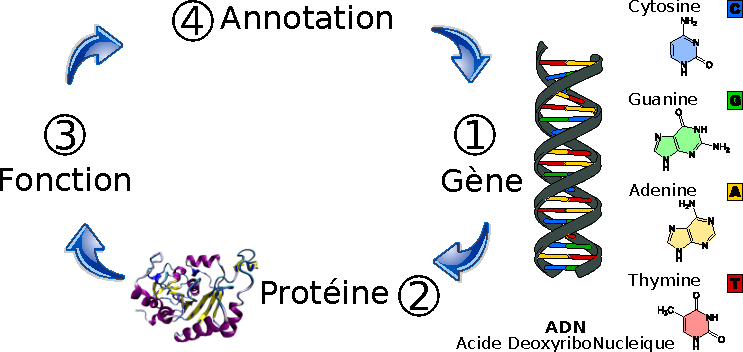
\includegraphics{img/simple_annotation_process.pdf}
    \caption{Vue globale du gène à l'annotation }
    \label{fig:glob_annotation}
\end{shadedfigure}

Des outils bio-informatiques analysent ces séquences afin de prédire les régions géniques et leurs fonctions dans l'organisme (voir \cref{fig:glob_annotation}). Selon les organismes, le nombre de gènes varie de quelques milliers à plusieurs dizaines de milliers de gènes. Ainsi, parmi le million voire milliard de paire de base d'\gls{ADN}, il faut identifier tous les gènes. Par conséquent, l'expertise humaine d'un génome est un défi en soi. Ces recherches se sont intensifiées et complexifiées, notamment avec la mise en place du projet d'étude de 100 000 génomes d'organismes pathogènes \cite{100kfoodborne}, ou encore l'analyse des eco-systèmes poly-microbiens présents sur l'Homme \cite{hmp}.

Pour se faire des outils bio-informatiques ont automatisé le traitement de l'information issue des séquenceurs afin de traiter un nombre d'organismes toujours plus grand. Ces outils, alimentés continuellement en nouveaux génomes, ont amplifié le déluge d'information. Dans le domaine de l'annotation fonctionnelle, moins d'un pour cent des données ont pu être vérifiées (au regard des statistiques publiées par UniProt et SwissProt en 2017 \parencites{uniprot_stat}{expasy_stat} ). Ce fossé entre information de confiance et prédiction s'accélère car il est plus rapide de produire de l'information que de la vérifier.

Or les prédicteurs automatiques de la fonction biologique des gènes ne sont pas fiables. En effet, 30\% des annotations fonctionnelles seraient incorrectes, voire 80\% dans certaines familles de protéines \parencites{devos2001intrinsic}{schnoes2009annotation}. Ces séquences incorrectement annotées sont ensuite propagées dans les bases de connaissances.

Une des méthodes d'assignation de fonction de gène, consiste à inférer une annotation provenant d'un gène connu à toutes les séquences similaires. En effet, il est supposé que l'évolution des produits des gènes sont sous pression de sélection afin de préserver leur fonction. L'ensemble des fonctions d'un organisme permet à ce dernier d'être adapté à son environnement. Étant donné qu'une modification d'un acide aminé impliqués dans la fonction peut potentiellement entrainer la perte de l'activité biologique. Et par conséquent mettre en péril les capacités de survit de l'organisme. Ces régions d'acides aminées devraient faiblement variées d'un point de vue physico-chimiques. Toutefois l'assimilation de proche en proche des fonctions biologiques tend à surestimé les propriétés biologiques d'une séquence. Car les séquences faussement annotées avec une fonction se retrouvent parmi les autres. Par conséquent, elles sont potentiellement utilisées, afin de propager une fonction d'un autre gène considéré similaire, détériorant un peu plus la qualité des bases de données.

L'objectif de l'annotation des fonctions géniques est de fournir un catalogue des capacités moléculaires et/ou biochimiques dont est pourvu un organisme. Ce catalogue permet de mieux comprendre le vivant. Cependant le processus d'annotation, produit et amplifie l'assignation de fonctions erronées à de nouveaux gènes et entraîne l'incapacité à utiliser ces prédictions sans prendre un risque. Le catalogue de fonctions géniques est en effet utilisé par la suite dans de nombreux domaines, comme l'étude des voies métaboliques, la biologie des systèmes, la classification des gènes essentiels et autres\ldots~Cette problématique impacte notre compréhension du vivant et notre capacité à l'étudier, remettant en cause tout le processus d'annotation des gènes utilisés jusqu'alors.

Face à cette problématique des approches variées ont été développés. On distingue les systèmes d'annotations automatiques à base de règle, reprenant le raisonnement appliqué par les bio-curateurs, comme le projet HAMAP \cite{lima2009hamap}. Ces règles sont généralement basées sur la séquence génomique et la taxonomie de l'organisme. Elles peuvent être créées par un bio-curateur ou par des outils d'apprentissage \cite{uniprot2011ongoing}.

On retrouve également les systèmes de reconstruction des voies métaboliques \cite{karpe2011pathway}. Ces méthodes utilisent des génomes complétement séquencés et bien annoté pour décrire des cascades de réactions amenant à un composé d'intérêt biologique.  Cette successions de réactions met en lumière un chemin à dans le réseaux de réactions, d'où le terme anglais "pathway" pour décrire un chemin qui amène à un objectif biologique. Par la suite, ces voies métaboliques identifiées sont proposées pour d'autres organismes dont l'annotation est partielles. Certains objectifs biologiques vont apparaître manquant au regards des prédictions sur les capacité métaboliques de l'organisme. Ces réseaux de concept forment un graphe de connaissance, spécifique de l'organisme. Ainsi, des fonctions marquées comme manquantes, à la réalisation de voie métabolique, sont suggérées aux bio-curateurs.

Les méthodes à base de règles automatisent l'annotation fonctionnelle par l'utilisation de règles liées à la biologie de l'organisme et non plus uniquement par une prédiction \textit{in silico}. Les méthodes, utilisant la représentation des connaissances biologiques, contextualisent les prédictions. De plus, elles permettent de suggérer des annotations fonctionnelles ne pouvant pas être détectées par les prédicteurs usuels. Toutefois, le travail de curation des annotations par un bio-curateur est nécessaire mais considéré comme fastidieux, laborieux et source d'erreur. Il apparaît nécessaire de fournir un assistant à la curation des fonctions géniques.

\section*{La démarche suivie dans cette thèse}

Mon travail de recherche s'est ouvert à de nombreuses disciplines afin d'apporter une méthode d'expertise des observations vis-à-vis du savoir, en biologie. En effet, la complexité du problème, nécessite l'intervention de concepts provenant de la logique, la représentation des connaissances, la théorie des graphes, la bio-informatique et le métabolisme. Ainsi, j'ai étudié ces différents domaines, décrypté le jargon, recherché les méthodes semblant avoir une application. Puis, je les ai combinées dans le but d'obtenir une méthode fiable et rapide.

Certaines voies furent des impasses, d'autres n'avaient pas encore de solution. À travers ces quelques chapitres je vous livrerai les notions et mon expérience sur ces différents domaines.

Cette thèse débute avec une problématique biologique \textit{"Comment guider et faciliter le travail des bio-curateurs, lors des étapes de l'annotation fonctionnelle ?"}. Pour cela, on souhaitait reprendre un prototype de vérification de la cohérence globale de l'annotation. En effet, l'équipe HELIX dirigé par \textit{Alain Viari} a travaillé sur une telle question. Leur projet a abouti à un raisonneur nommé HERBS. Cet outil permet de déterminer les concepts biologiques attendues et correctement prédits des autres concepts. Nous devions donc étendre ces fonctionnalités afin de prendre en compte l'incertitude et la contradiction. À ce moment nous pensions que le travail consistait à récupérer les méthodes logiques, puis de les adapter à la biologie, puis mettre à jour l'outil. Or à aucun moment, nous nous doutions que certaines problématiques de la logique, étaient toujours ouvertes. En effet, la logique a ses limites, notamment lorsque l'on travaille avec des concepts, dont certains peuvent prendre des états ni-vrai-ni-faux. Ou encore, lorsque l'on souhaite raisonner sur des ensembles d'ensemble. Comme je l'ai compris plus tard, le monde de la logique a été rythmé par des faits marquants comme le paradoxe de \textit{Russell}. Tel un historien, je me suis retrouvé dans les grandes problématiques de la logique moderne. Ainsi j'ai suivi les traces, de \textit{Platon} avec les bases de la logique classique, \textit{Bertrand Russell} pour les ensembles, \textit{Jan Łukasiewicz} et le principe de tiers exclu, \textit{Nuel Belnap} et la logique à quatre valeur.

\note{Le paradoxe de Russell démontre que si un ensemble est membre de lui-même, alors par définition il ne peut être un membre de lui-même. Mais s'il n'est pas un membre de lui-même, alors il est un membre de lui-même.
    
    Le paradoxe du barbier image une telle situation. Imaginer, Le conseil municipal d'un village vote un arrêté municipal qui enjoint à son barbier (masculin) de raser tous les habitants masculins du village qui ne se rasent pas eux-mêmes et seulement ceux-ci.
    
    Le barbier, qui est bien un habitant du village, n'a pas pu respecter cette règle car :
    \begin{itemize}
        \item S'il se rase lui-même, il enfreint la règle, car le barbier ne peut raser que les hommes qui ne se rasent pas eux-mêmes ;
        \item S'il ne se rase pas lui-même - qu'il se fasse raser ou qu'il conserve la barbe - il est en tort également, car il a la charge de raser les hommes qui ne se rasent pas eux-mêmes.
    \end{itemize}
}

D'autre part, il apparut très tôt la nécessité de représenter le savoir, dans un modèle générique. Permettant ainsi d'avoir un modèle, utilisable pour le plus grand nombre d'entrepôts de données. Cette recherche commença par les travaux de John F. Sowa sur la représentation des connaissances ( \citeyear{sowa92,sowa99}).

Le défi est de représenter des connaissances, sans a priori sur la représentation des données dans les entrepôts de données. Pour cela, un travail de structuration des concepts et de classification de leurs relations a été mené. Ce travail m'a amené à étudier la logique de description \cite{baader2003description}. Concrètement ce domaine de recherche permet de faire le lien entre l'intelligence artificielle et la représentation du savoir. L'étude portée sur cette représentation du savoir est un sujet très dynamique, avec l'essor du \textit{Web Semantic}. Cette thématique se consacre à l'étude de la nature des concepts, de leur relations, mais également de leur existence définissant par la même l'ontologie.

Dans l'objectif de cartographier notre savoir en Biologie, un consortium international s'est créé : \textit{\gls{GO}} (voir G. O. Consortium
et al \citeyear{go2001,go2004}). Les concepts sont classifiés parmi trois catégories distinctes (i) les fonctions moléculaires, (ii) les processus biologiques et (iii) les composants cellulaires. Les concepts sont appelés des GO termes. Les relations entre les termes porte des étiquettes pour exprimer les notions de composition et de type \cref{fig:go_relation}. Ces descriptions de connaissances sont effectuées avec un langage contrôlé.  C'est à dire que le vocabulaire et la grammaire est restreinte, afin de réduire l'ambiguïté et donc la complexité des textes. Un tel langage permet à un programme informatique de comprendre une phrase. Ainsi cet ensemble de mot peut être utilisé pour vérifier la cohérence du texte. Ou encore un utilisateur peut effectuer des interrogations sur l'ensembles des connaissances décrites.

Figure ici: ftp://ftp.geneontology.org/pub/go/www/GO.ontology.relations.shtml


La structure des données répondait à nos besoins. Cependant le lien entre les termes d'une catégorie avec une autre n'était pas fourni. Par exemple on ne peut pas relier des processus biologiques à des fonctions moléculaires. Des projets comme \cite{AdditionalGO2006} parviennent partiellement à couvrir les liens  entre les termes des différentes catégories.

Toutefois, un nombre trop important de relation restait manquante. Pour cette raison, j'ai mis au point une structure de concept avec toutes les notions nécessaires afin de représenter nos connaissances. Cette structure sera le support d'inférence des observations biologiques. L'objectif étant de vérifier l'existentialité de nos connaissances sur chaque organisme.

Tout au long de mon travail de recherche j'ai été confronté à des limites. Si bien que des solutions nouvelles devaient être inventées. La problématique d'apparence simple s'est révélée plus complexe. Ainsi, j'ai dû rechercher des notions dans des domaines "éloignés" de la bio-informatique comme \textit{la Logique}. Établir un modèle générique afin de représenter toute sorte de données, même celle auxquelles je n'aurais pas pensé ! J'ai également mis en place des méthodes permettant d'intégrer un volume de donnée conséquent tout en étant capable de fournir un résultat dans un temps raisonnable. Ce travail m'a demandé de dépasser les paradoxes de la logique afin de l'étendre aux notions d'inconnu et de contradiction. De sorte que la méthode finale puisse proposer des annotations manquantes, mettre en lumière les contradictions, de vérifier les prédictions \textit{In-Silico} avec les expectations biologiques, explorer les capacités métaboliques de tout organisme.

Pour cela, la suite de cette thèse commence par une présentation des concepts métaboliques et de leurs représentations informatiques. Puis, les liens entre génome et métabolisme seront détaillés. Pour continuer sur les données biologiques dont nous disposons. Suivi par des notions sur la \textit{Logique} et l'\gls{IA}. On continuera par les systèmes experts, utilisé pour résoudre des problèmes biologiques. Ceci, introduira le début de GROOLS. Mais également, les problématiques qui étaient restés ouvertes jusqu'alors. Afin de parvenir aux notions de raisonnement descriptif avec la méthode mise en œuvre dans GROOLS, cette thèse se termine par la présentation des résultats et les pistes de recherches envisagées.


\subbibliography
\end{refsegment}
    
    \begin{refsegment}
	\chapter{Contexte biologique et méthodologique}

    Ce chapitre présente les notions biologiques puis informatiques, utilisées comme fondement du travail de recherche effectué lors de cette thèse.
    
    
    \section{Le métabolisme et sa représentation informatique}
    \subsection{Généralités sur le métabolisme}
    
    Pour perpétuer son espèce, tout organisme vivant consomme de l'énergie pour produire de la biomasse et se répliquer. Pour cela, l'être vivant doit assimiler des composés présent dans son environnement. Ces composés chimiques lui permettent de produire l'énergie, nécessaire à la survie mais surtout à la transmission du patrimoine génétique. Ainsi on désigne par métabolisme, l'ensemble des processus de synthèse et dégradation de composés chimiques, mis en œuvre par l'organisme. 
    
    \note{Le mot métabolisme à évolué à travers l'histoire pour nous parvenir sous ça forme actuelle. En grec ancien on utilise "\greekFont{μεταβολή}" équivalent à metabolé désignant "transformation". Le mot métabole signifie "qui subit un changement". Il a été utilisé par la suite comme mot racine: métabol-ique, métabol-isme \ldots
    }
    
    Les organismes vivant opèrent une multitude de transformations chimiques. Ils forment de véritables usines de traitement biochimique. En effet, ils disposent d'une batterie de réactions biochimiques, afin de traiter un grand nombre de composés, tant à l'intérieur qu'à l'extérieur de la cellule. Par exemple, certains composés, de par la nature de la membrane cellulaire \footnote{La membrane cellulaire constitue une barrière physique entre le milieu extérieur et intérieur de la cellule.} ou leur toxicité, doivent être transformés depuis l'extérieur de la cellule, afin d'être assimilés. De ce fait, la matière présente dans l'environnement est utilisé pour constituer les briques nécessaires au vivant.
    
    Effectivement, le métabolisme est essentiel à la vie: d'une part il fournit l'énergie nécessaire et d'autre part, il va produire les molécules de base indispensables à l'organisme à sa construction, sa défense et autres \ldots
    
    Bien qu'agissant à une échelle moléculaire, le métabolisme d'un groupe d'organismes peut impacter son environnement. Si bien que les conséquences peuvent être observées à l'échelle humaine voire, dans certains cas à l'échelle de la planète (voir Figure~\cref{fig:bloom}). Un autre exemple est celui des espèces végétales. Elles absorbent du dioxyde de carbone et produisent de l'oxygène. Ainsi elles jouent un rôle important dans la concentration de ces composés dans l’atmosphère.
    
    
    \begin{shadedfigure}[H]
        \begin{subfigure}[b]{.5\textwidth}
            \centering
            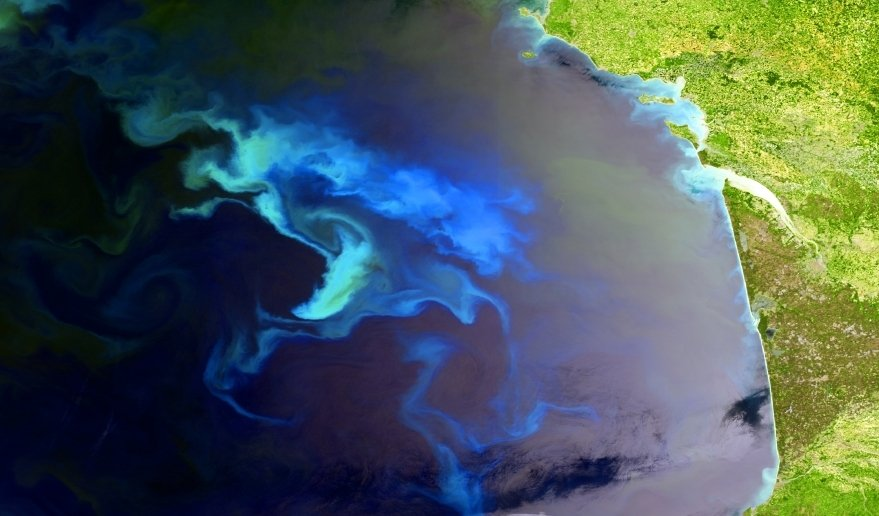
\includegraphics[width=\textwidth]{img/bloom_gascogne.jpg}
            \caption{{\tiny Source: \url{http://seos-project.eu}}}
            \label{fig:bloom_gascogne}
        \end{subfigure}
        \hfill
        \begin{subfigure}[b]{.5\textwidth}
            \centering
            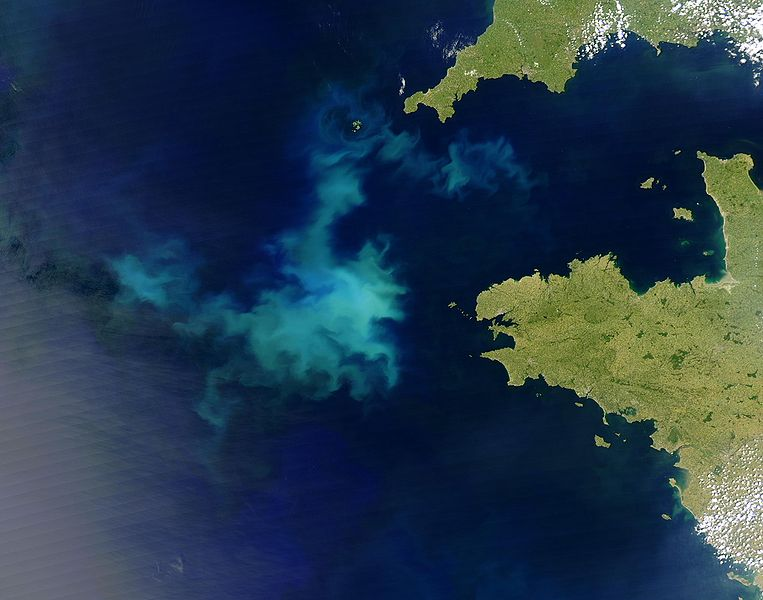
\includegraphics[width=\textwidth]{img/bloom_bretagne.jpg}
            \caption{{\tiny Source: \url{https://commons.wikimedia.org/}}}
            \label{fig:bloom_bretagne}
        \end{subfigure}
        \caption{Les activités métaboliques d'un groupe d'individus produit une quantité de pigments photosynthétiques suffisamment conséquentes, qu'il en devient observable depuis l'espace. Deux événements distincts sont représentés. Le premier a eu lieu au large de la Gascogne le 17 mai 2004 et le second au niveau de la Bretagne le 15 juin 2004.}
        \label{fig:bloom}
    \end{shadedfigure}
    
    \note{Lors de l'apparition des premières formes de vie, il y a 3,6 milliards d’années, l'atmosphère était faiblement pourvue en oxygène. Des organismes anaérobies étaient présents dans les océans. L'oxygène est toxique, leur métabolisme s'est adapté au dioxyde de carbone présent abondamment à ce moment. Puis entre 3,5 à 3 milliards d'années apparurent des cyanobactéries. Ce sont des bactéries capables de capter l'énergie du soleil. Elles sont "photosynthétiques". Leurs métabolismes possèdent la particularité d'oxyder les minéraux présents dans les océans. Elles produisent ainsi de l'oxygène. Avec le temps leur métabolisme a consommé tellement de minéraux que l'oxygène produit dans les océans s’est libéré dans l’atmosphère. \textit{De facto} la proportion des gaz atmosphériques fut bouleversée. Cet événement influença le cours de la vie, de sorte qu'un certain nombre d'organismes s'adaptèrent à l'oxygène. Car l'oxygène devient alors une molécule courante. Certaines formes de vie évoluèrent jusqu'à devenir aérobie. Avec cet événement, la Terre a subi sa première pollution atmosphérique d'ampleur induite par des organismes vivants. (Lire: \citetitle{bengtson1994early} ) }
    
    \subsection{Les acteurs}\label{subsec:acteurs}
    
    L'étude du métabolisme est essentielle pour la compréhension des êtres vivants. Les applications impactent de nombreux domaines, tels que : l'industrie pharmaceutique, l'énergie, l'agriculture, l'environnement\ldots.  Pour mieux le comprendre, il est nécessaire d'introduire les différents acteurs du métabolisme. En effet, le métabolisme représente un ensemble d'événements faisant intervenir des métabolites, des réactions, des cofacteurs, des enzymes. Ces intervenants sont représentés dans les voies métaboliques.
    
    
    
    \subsubsection{Les métabolites}
    
    Ce sont des composés organiques, de petite taille, produits à travers les différents processus issus du métabolisme. Ils sont tour à tour synthétisés puis dégradés. Selon leurs rôles, ils interviennent soit dans les processus indispensables au développement et à la reproduction, dit "métabolisme primaire"; soit dans des fonctions non vitales comme la production d'antibiotiques, de phéromones, de pigments \ldots, dénommées "métabolisme secondaire" .
    
    \note{Un composé organique s'oppose à un composé minéral. Cette différenciation s'explique par des raisons philosophiques antérieur au \siecle{19}. En effet, on distinguait les substances constitutives des organismes, des autres. Ces autres autres molécules semblaient nécessaires à la vie, pour autant on ne savait pas les synthétiser. Pour ces raisons, on expliquait à cette époque que l'intervention d'une "force vitale" était nécessaire pour produire ces molécules. En 1828, Friedrich Wöler mis au point accidentellement, une expérience produisant de l'urée (considéré comme organique) à partir de composés minéraux, comme le cyanate d’ammonium. Depuis lors, la notion de composé organique a évolué afin de désigner une molécule constituée d'une partie de carbone, le reste pouvant être des atomes d'hydrogène, d'oxygène, d'azote et autres. La notion organique est restée car le carbone est un élément essentiel du vivant. Par opposition, un composé minéral correspond à toutes molécules constituées d'éléments autres que le carbone. Pour plus d'information, je vous invite à lire \citetitle{chimie_organique}.
    }    
      
	\subsubsection{Les réactions}
	Le processus de transformation d’un métabolite est décrit par une réaction. On désigne par le terme "substrat", les métabolites avant transformation. Par opposition, on parle de produit pour la molécule transformée. Ainsi une réaction est l'événement qui va transformer un substrat afin de produire un nouveau métabolite. Ces réactions s'effectuent au sein de l'organisme, dans l'infiniment petit, au niveau moléculaire.
    
    Une réaction est généralement représentée par une équation constituée à gauche, de la somme des molécules nécessaires à la transformation et à droite de la somme des molécules produites (voir \cref{fig:reaction}). Cette équation  représente la stœchiométrie de la réaction. C’est-à-dire que la proportion des éléments en jeu avant et après la réaction est respectée. De telles réactions sont représentées à l'équilibre, c'est-à-dire que la proportion de chaque atome est identique avant et après la réaction. Pour reprendre la célèbre maxime "Rien ne se perd, rien ne se crée, tout se transforme" .
    
    \begin{shadedfigure}[H]
        \centering
        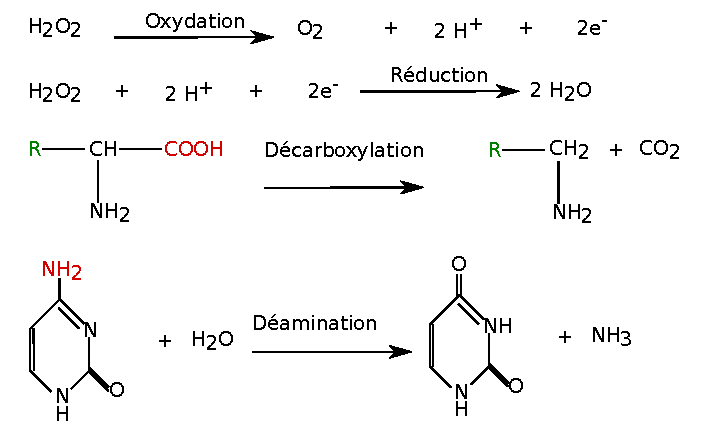
\includegraphics[width=\textwidth]{img/equation_reaction.pdf}
        \caption{Représentation de réaction sous leur forme "équation-bilan" .}
        \label{fig:reaction}
    \end{shadedfigure}
    
    \citation{ [\ldots] On voit que, pour arriver à la solution de ces deux questions, il fallait d'abord bien connaître l'analyse et la nature du corps susceptible de fermenter, et les produits de la fermentation ; car rien ne se crée, ni dans les opérations de l'art, ni dans celles de la nature, et l'on peut poser en principe que, dans toute opération, il y a une égale quantité de matière avant et après l'opération ; que la qualité et la quantité des principes est la même, et qu'il n'y a que des changements, des modifications }{Antoine Lavoisier}[Traité élémentaire de chimie, 1864]
    
    
    \subsubsection{Les enzymes}    
    La plupart de ces transformations ne sont pas spontanées ou se feraient trop lentement. Pour cela, l'organisme dispose de molécules protéiques facilitant ces transformations, appelées "enzymes". Ce sont des bio-catalyseurs, c'est-à-dire qu'elles vont favoriser ou accélérer une transformation chimique. Ces molécules peuvent couper, coller, réparer synthétiser ou encore modifier une molécule. Elles ont la particularité d'avoir une forte affinité avec leur substrat.  Leur rencontre provoque une transformation du composé. Puis le ou les produits résultant de cette transformation, peuvent être à leur tour reconnus par d'autres enzymes. Provoquant ainsi une cascade de transformations chimiques. 
    
    Une enzyme est une protéine, dont sa structure tri-dimensionnelle contient des régions impliquées dans la reconnaissance et la transformation d’une molécule. C'est pourquoi, une même enzyme reconnaît une ou plusieurs molécules spécifiquement et induit les mêmes transformations chimiques. Ce processus est décrit par le modèle de "clef / serrure" (voir \cref{fig:reaction_enzymatique}). Le plus couramment les activités enzymatiques sont répertoriées selon quatre numéros séparés par des points. C'est le système de nomenclature \acrfull{EC}. Chaque nombre est associé à un concept. Ainsi le premier indique la classe de la réaction catalysée, le second décrit la catégorie du substrat utilisé, le troisième correspond à la nature de la réaction et enfin le quatrième est le numéro de série de l'activité enzymatique.
    
    \begin{shadedfigure}[H]
        \centering
        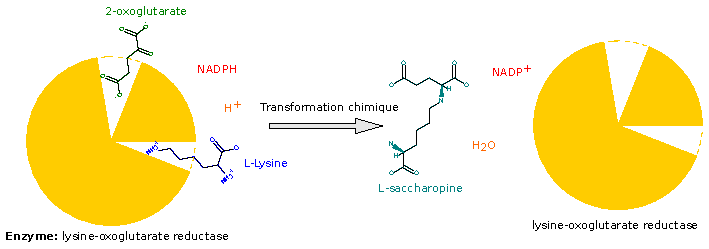
\includegraphics[width=\textwidth]{img/lysine-oxoglutarate_reductase.pdf}
        \caption{Schéma d'une réaction chimique catalysée par une enzyme. L'enzyme reconnaît ses substrats 2-oxoglutarate et L-Lysine, puis les transforme en une molécule de L-Saccharopine. La molécule NADPH$^{+}$ est nécessaire à l'activité enzymatique. On parle de cofacteur.}
        \label{fig:reaction_enzymatique}
    \end{shadedfigure}
    
    Une enzyme possède une affinité importante pour son substrat. Cette affinité influe sur l’activité enzymatique, c’est-à-dire sur la vitesse de transformation du substrat. D'autres molécules possèdent également une forte affinité pour l’enzyme et par conséquent rentre en compétition avec les substrats de l'enzyme. De tels molécules vont diminuer l’activité enzymatique voir dans certains cas l'arrêter. On parle alors d'inhibiteurs enzymatiques. Ces inhibiteurs jouent un rôle important dans le métabolisme. Ils sont employés comme régulateurs du métabolisme. 
    
    \note{
        Les inhibiteurs enzymatiques permettent de limiter voir d’arrêter l’activité d’une enzyme. Cette caractéristique est employée pour  tuer des organismes pathogènes. Par exemple, La Pénicilline est un inhibiteur de la  transpeptidase intervenant dans la synthèse du peptidoglycane. Le peptidoglycane forme la paroi des bactéries. Si cette dernière est dans l’incapacité de synthétiser sa paroi alors elle meurt.
    }

    \subsubsection{Les cofacteurs}
    Certaines réactions nécessitent l’apport d'énergie, d’ion ou encore de molécules "d'assistance" qui vont favoriser l’activité enzymatique. Les enzymes nécessitant l'apport de cofacteur sont appelées holoenzymes lorsque le cofacteur est lié à cette dernière. Par opposition, une enzyme inactive non liée à son cofacteur est une apoenzyme. Les cofacteurs sont classifiés en deux catégories : les ions métalliques et les coenzymes.
    
    Les ions métalliques de par leurs charges positives permettent de contre-balancer les charges négatives apportées soit par les chaînes d'histidines de l'enzyme, soit lors de la réaction catalytique \cite{christianson1991structural}. Dans le premier cas l'ion métallique joue un rôle structural au sein de l'enzyme. Dans le second, il va assister l'enzyme dans son processus de transformation tout en maintenant sa structure. Effectivement, les ions métalliques de part leur nature, peuvent assister l'enzyme lors des réactions d'oxydoréduction et de transfert d'électron. Les ions fréquemment observés dans le vivant sont les ions fers, cuivres, zincs et magnésiums.
    
    Les coenzymes sont des molécules organiques. Elles sont rangées en deux groupes en fonction de la nature de la liaison établie avec l'apoenzyme.
    
    Le premier groupe contient les cofacteurs liés faiblement à l'enzyme. Ces cofacteurs subissent généralement une transformation lors de la réaction. Pour cette raison ils sont également appelés co-substrat. Par exemple une des réactions de la glycolyse implique le cofacteur NADP$^{+}$ pour transformer le glucose-6-phosphate (voir l'équation \ref{eq:glucose}). Ce cofacteur  se lie à l'enzyme puis il est transformé au cours de la réaction en NADPH. Cette modification engendre la libération du cofacteur de l'enzyme. Ce groupe contient également des cofacteurs énergétiques, c'est-à-dire que la transformation du cofacteur va engendrer une libération d'énergie. Cette énergie permet de réaliser des transformations qui étaient dans la cellule énergétiquement défavorable. De nombreux mécanismes essentiels au vivant nécessitent l'apport d'énergie. Pour ces raisons, le métabolisme d'un organisme est adapté à son environnement afin de produire l'énergie indispensable à sa survie et sa reproduction. Majoritairement, le nucléotide \acrfull{ATP} est utilisé par le vivant comme cofacteur énergétique. L'hydrolyse de l'\acrfull{ATP} en \acrfull{ADP} induit la coupure d'une liaison avec un phosphate provoquant une libération d'énergie. On retrouve également d'autres cofacteurs utilisant la guanine, la thymine, la cytosine ou encore l'uracile en lieu et place de l'adénine (respectivement  GTP, TTP, CTP et UTP ). Le vivant est en perpétuel déséquilibre énergétique dû aux différents processus consommateurs d'énergie qui le constitue. De ce fait, l'apport énergétique permet le maintien de la vie.
    
    \begin{equation}\label{eq:glucose}
        glucose-6-phosphate + NADP^{+} \rightarrow 6-phosphoglucono-D-lactone + NADPH + H^{+}
        \stepcounter{equation}\tag{équation \theequation}
    \end{equation}
    
    Le deuxième groupe de coenzyme représente les cofacteurs liés de façon covalente \footnote{Une liaison covalente est une liaison chimique dans laquelle deux atomes sont mutuellement attirer par une force. Cette force provient de la mise en commun d'au moins un électron par atome.} à l'enzyme. Ils sont appelés "groupements prosthétiques". Un des exemples les plus connus et celui de l'hème des hématies. C'est un groupement contenant un atome de métal (souvent le fer) permettant de capturer un gaz diatomique comme le dioxygène (O${2}$) où encore le monoxyde de carbone (CO).
    
    Ainsi, le vivant à travers ces différents acteurs possède une multitude de réactions lui procurant les moyens de vivre et de se reproduire. Ces successions de réactions sont représentées selon des objectifs considérés d'intérêt biologique. Pour cette raison un cheminement de transformations métaboliques est appelé "voie métabolique".
    
    
    \subsubsection{Voies métaboliques}
    On distingue dans le métabolisme deux catégories de processus, l'anabolisme et le catabolisme. L'anabolisme représente l'ensemble des réactions impliquées dans la synthèse de nouvelles molécules. La production de nouveaux composés nécessite de l'énergie. De tels processus sont constitués de réactions endergoniques. Ainsi le bilan énergétique est négatif.  Au contraire, le catabolisme décrit l'ensemble des réactions de dégradation de molécules. Les réactions, impliquées dans la dégradation d'un composé, produisent \textit{in-fine} plus d'énergie qu'elles en ont consommée. Ces réactions sont dites exergoniques.
    
    Ces notions permettent de diviser l'ensemble des processus du métabolisme en sous-parties plus faciles à appréhender. Les réactions sont regroupées dans différentes entités appelées "voies métaboliques". Ce découpage permet de représenter des segments d'événements de transformations métaboliques en ensemble de réactions permettant de réaliser un objectif d'intérêt biologique. Certains objectifs peuvent être atteints de plusieurs manières. Ainsi une même voie métabolique peut être réalisée par différents chemins de réactions. Pour décrire ces chemins, généralement on utilise le terme de "variant".
    
    Le vivant est soumis à des contraintes liées à son environnement. Par conséquent, des modules métaboliques conférant des avantages à un organisme vont tendre à être sélectionnés. Cette pression sélection induit que ces modules métaboliques vont être conservés à travers les générations \cite{braakman2012compositional}. Les gènes correspondant aux protéines impliquées dans ces voies sont souvent co-localisés sur le génome. En effet, une telle disposition des gènes favorise l'expression de toutes les protéines nécessaires à la réalisation de l'objectif biologique à un instant "\textit{t}". Cette organisation "opéronique" simplifie le processus de régulation de l'expression des gènes. 
    
    Comprendre la structuration du métabolisme, c'est également expliquer comment la physique et la chimie ont contraint la vie et l'évolution.
    
    Ces voies métaboliques sont des réactions connectées les unes aux autres. Elles se représentent intuitivement sous forme de graphe.
    
    \subsection{Représentation en graphe}
    
    De telles représentations permettent de partager des notions complexes sur un grand nombre de concepts ainsi que leurs relations. Les graphes s'avèrent utiles pour l'étude de divers réseaux. Par exemple, la représentation d’un réseau routier en graphe est intuitive et permet, par exemple, la mise en œuvre d'algorithmes de recherche du plus court chemin. Cette branche des mathématiques s'est illustrée à travers la résolution de problèmes complexes comme la traversée des sept ponts de Königsberg, la marche du cavalier sur l’échiquier et bien d'autres. Les applications des recherches issues de la théorie des graphes sont multiples. On retrouve son utilisation dans des domaines comme la chimie, le stockage de données (à travers les bases de données type graphe), les ontologies, la biologie et ses différents réseaux (dont le métabolisme). Cette représentation de l'information a montré son utilité à des problèmes complexes très variés.
    
    Avant d'aller plus loin, il est nécessaire de définir plusieurs notions employées dans la théorie des graphes. Tout d'abord un graphe est constitué de nœuds reliés entre eux. Les nœuds du graphe sont également appelés sommets ("vertice" ou "node" en anglais).  Lorsque les relations indiquent un sens de cheminement entre deux nœuds ("edge" en anglais), elles sont qualifiées d'arc, autrement on parle d'arête. Ainsi, on fait la distinction entre graphe orienté et non-orienté. Généralement un graphe est désigné sous la forme mathématique :
    
    \begin{equation}\label{eq:graph}
    	G = (V,E) \stepcounter{equation}\tag{équation \theequation}
    \end{equation}
    
    Dans l'équation \ref{eq:graph}, G désigne le graphe tel que constitué de deux ensembles, celui des sommets V et celui des relations V. Différents types de graphe sont présentés dans la \cref{fig:graphe}.
    
    
    \begin{shadedfigure}[H]
    	\centering
    	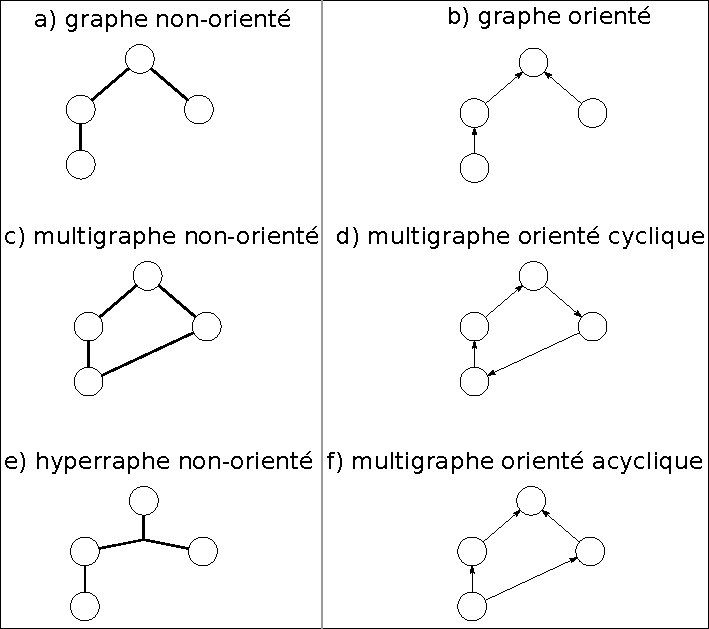
\includegraphics[width=\textwidth]{img/graph.pdf}
    	\caption{a) un graphe  avec des arêtes. b) Un graphe avec des arcs indiquant une orientation entre deux sommets. c) un multigraphe non orienté avec des arêtes étiquetées reliant les deux mêmes sommets. d) un graphe dont les relations forment un chemin cyclique à travers les sommets. e) un graphe avec une hyper-arête reliant deux sommets. f) un graphe avec une orientation des relations telles que le chemin à travers le graphe ne traverse qu'une seule fois les sommets. }
    	\label{fig:graphe}
    \end{shadedfigure}
    
    
    
    Dans le cadre de la biologie, de nombreux événements se représentent sous forme de réseaux. Pour en citer quelques-uns, il y a les réseaux d'interactions physiques protéine-protéine, de régulation de l'expression des gènes, de maximisation de flux (\acrfull{FBA}), de réactions métaboliques. 
    
    On peut représenter un réseau métabolique sous différentes formes de graphe :
    \begin{itemize}
    	\item Réseau de métabolites : les nœuds représentent les composés chimiques et deux nœuds sont liés par une arête s'il existe une réaction qui permet la transformation du premier métabolite en deuxième
    	\item Réseau de réactions : les nœuds représentent les réactions et deux nœuds sont reliés s’il existe un composé chimique produit par la première réaction substrat de la deuxième.
    	\item Réseau de métabolites et de réactions : un graphe biparti où les nœuds sont de type composé ou réaction et reliés par des arêtes permettent de passer d’un type à l’autre.
    	
    \end{itemize}
    Dans ce chapitre, nous allons nous intéresser à la représentation en graphe des voies métaboliques. 
    
    \subsection{Ressources sur les voies métaboliques}
    
    Une voie métabolique est un enchaînement de réactions enzymatiques durant lequel les métabolites sont transformés. Elle représente usuellement une fonction biologique. Par conséquent ces fonctions sont susceptibles d'être partagées à travers le monde du vivant. Toutefois pour réaliser une fonction biologique, il peut exister plusieurs variantes de chemins réactionnels. Par exemple, pour la biosynthèse de la L-lysine, six voies alternatives sont connues à ce jour dans le monde du vivant (voir \cref{fig:lysine} ).
    	
    	
   	\begin{shadedfigure}[H]
   		\centering
   		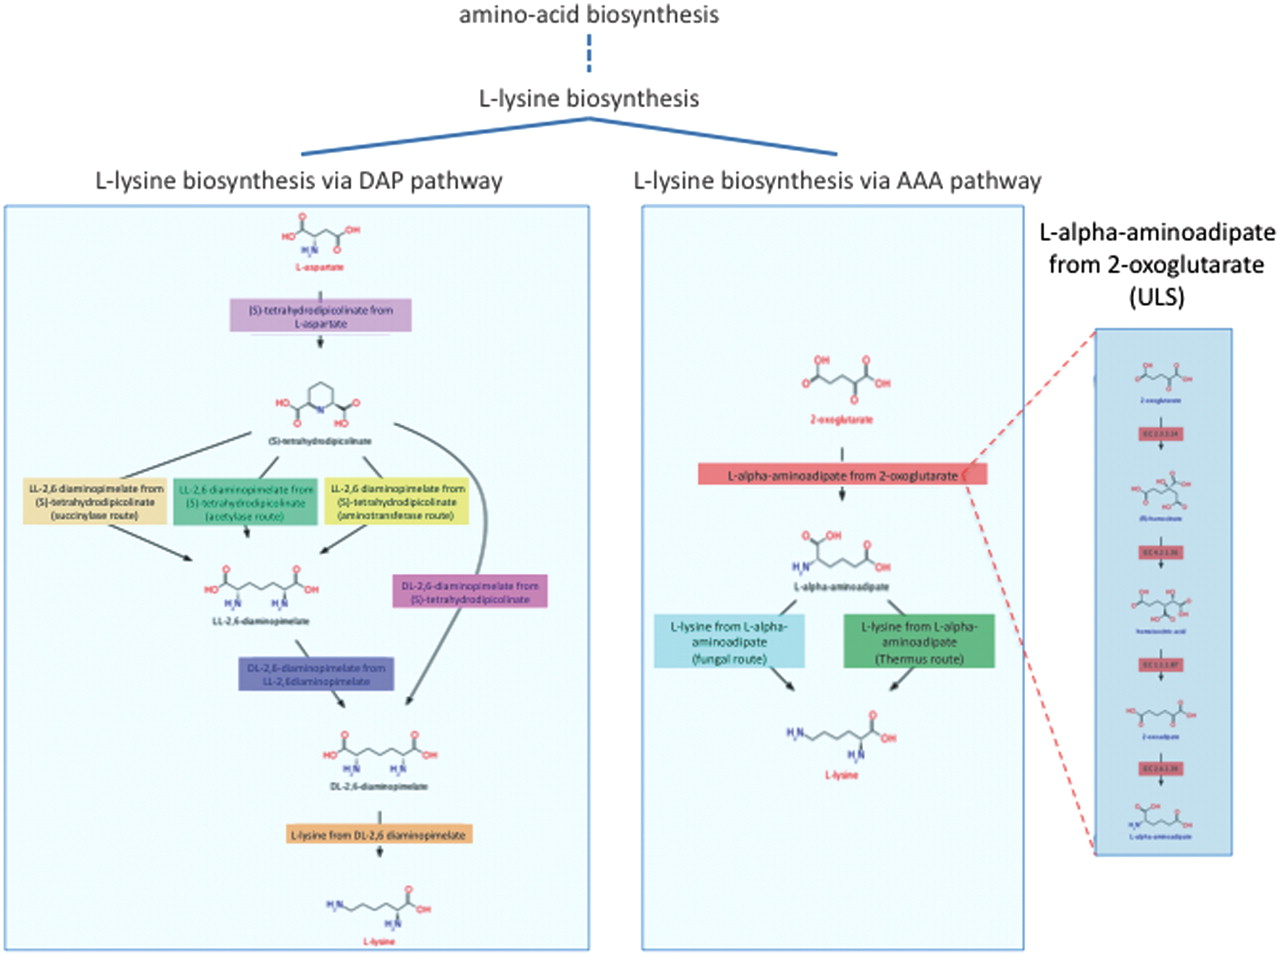
\includegraphics[width=\textwidth]{img/L-lysine-biosynthesis.jpg}
   		\caption{La biosynthèse de la L-Lysine peut se faire par via la voie DAP et ses quatre chemins de réactions possibles où via la voie AAA et ses deux voies alternatives. Figure reprise de l'article \citetitle{morgat2011unipathway}. }
   		\label{fig:lysine}
   	\end{shadedfigure}
     
     La représentation des voies métaboliques est une synthèse d'événements se produisant dans le vivant. Par conséquent cette représentation est subjective. Elle diffère selon les éléments mis en avant ou bien encore selon les informations et les meta-informations dont dispose la ressource. Ces différences seront exposées au cours de la présentation des principales ressources sur les voies métaboliques \texttt{\gls{KEGG}}, \texttt{Reactome}, \texttt{Unipathway}, \texttt{MetaCyc}.
     
    \subsubsection{KEGG}
    
    La ressource \texttt{\gls{KEGG}} \cite{ogata1999kegg,kanehisa2000kegg,kanehisa2002kegg,kanehisa2004kegg,aoki2005using,kanehisa2010kegg,kanehisa2017kegg} est une ressource de données permettant d'étudier les fonctions biologiques. Certaines connaissances portent sur la cellule, d'autres sur des entités plus grandes comme l'organisme et même sur  des écosystèmes. Pour cela \texttt{\gls{KEGG}} dispose d'un point d'entrée principal \url{http://www.genome.jp/kegg/kegg2.html}. Ce point d'entrée liste les trois orientations proposées par\texttt{\gls{KEGG}}.
    
    La première entrée est "orientée donnée", elle comprend les informations relatives à : la biologie des systèmes\footnote{Domaine d'étude pour la compréhension des interactions entre les différentes parties du système biologique, tels que les réseaux de gènes et de protéines, les organites et autres \ldots. } , la génomique, la chimie et la santé (voir le détail dans le \cref{tab:kegg_data_oriented}). Le second point d'entrée dit "sujet orienté" propose des informations relatives à une thématique comme le cancer (\textit{KEGG Cancer}), les pathogènes (\textit{KEGG Pathogen}), les virus (\textit{KEGG virus}) et autres. Le dernier point d'entrée correspond aux informations spécifiques à un organisme via \textit{KEGG organism}. Ce catalogue contient les génomes complétement séquencés de 346 eucaryotes, 4039 bactéries et 243 archées.  
    
    
    \begin{table}[H]
        \small
        \caption{Détail du point d'entrée "orienté donnée". }\label{tab:kegg_data_oriented}
        \label{tab:kegg_oriented_data} 
        \begin{tabular}{p{0.2\linewidth}|p{0.3\linewidth}|p{0.5\linewidth}}
            \toprule
            Catégorie               & Point d'entrée                                                        & Contenu \\
            \midrule
            Biologie des systèmes  & \href{http://www.genome.jp/kegg/pathway.html}{KEGG PATHWAY}            & Carte métabolique \\   
            \cline{2-3}
                                    & \href{http://www.genome.jp/kegg/brite.html}{KEGG BRITE}               & Structuration hiérarchique de fonctions biologiques \\
            \cline{2-3}             & \href{http://www.genome.jp/kegg/module.html}{KEGG MODULE}             & Collection d'unités fonctionnelles utilisées pour l'annotation génomique et l'interprétation biologique \\
            \hline
            Génomique               & \href{http://www.genome.jp/kegg/genome.html}{KEGG GENOME}             & Collection d'organismes \texttt{\gls{KEGG}} complétement séquencés. \\
            \cline{2-3}             & \href{http://www.genome.jp/kegg/genes.html}{KEGG GENES}               & Catalogue de gènes et protéines \\
            \cline{2-3}             & \href{http://www.kegg.jp/kegg/ssdb/}{KEGG SSDB}                       & Base de données sur la similarité des séquences d'acide aminé à partir de tous les gènes codant des protéines dont le génome est complet \\
            \cline{2-3}             & \href{http://www.genome.jp/kegg/ko.html}{KO (KEGG Orthology)}         & Association des fonctions biologiques aux différents groupes orthologues  \\
            \hline
            Chimie                  & \href{http://www.genome.jp/kegg/compound/}{KEGG COMPOUND}             & Ensemble de petites molécules d'intérêt biologique\\
            \cline{2-3}             & \href{http://www.genome.jp/kegg/glycan/}{KEGG GLYCAN}                 & Collection de structures de glycane expérimentalement observées \\
            \cline{2-3}             & \href{http://www.genome.jp/kegg/reaction/}{KEGG REACTION}             & Banque de données répertoriant les réactions chimiques dont les réactions enzymatiques\\
            \cline{2-3}             & \href{http://www.genome.jp/kegg/annotation/enzyme.html}{KEGG ENZYME}  & Catalogue d'enzymes associées                                                                                                                                                                                                                                                                                               à leurs numéros \acrfull{EC}\\
            \hline
            Santé                   & \href{http://www.genome.jp/kegg/disease/}{KEGG DISEASE}               & Fournit des cartes représentant les différents perturbateurs. Ces perturbateurs peuvent être géniques, infectieux, multi-factoriels \ldots\\
            \cline{2-3}             & \href{http://www.genome.jp/kegg/drug/}{KEGG DRUG}                     & Classification et description des drogues autorisées au Japon, USA et en Europe\\
            \cline{2-3}             & \href{http://www.genome.jp/kegg/drug/environ.html}{KEGG ENVIRON}      & Est une collection de médicaments, d'huiles essentielles et d'autres substances favorisant la santé, qui sont pour la plupart des produits naturels de plantes \ldots Cette base complète la ressource \textit{KEGG DRUG}.\\
            \cline{2-3}             & \href{http://www.genome.jp/kegg/medicus.html}{KEGG MEDICUS}           & Est une ressource faisant la synthèse des autres  bases orientées-santé \\
            \bottomrule
        \end{tabular}
    \end{table}
    
    
    Les différents acteurs du métabolisme sont répartis à travers les bases de données \textit{KEGG LIGAND} pour les métabolites, \textit{KEGG REACTIONS} pour les réactions et \textit{KEGG ENZYME} pour les enzymes.
    
    En ce qui concerne la représentation du métabolisme, \textit{KEGG PATHWAY} organise le réseau métabolique en un graphe dirigé (voir \cref{fig:kegg_lysine}). Ce réseau est découpé sous forme de cartes répertoriant toutes les réactions supposées avoir lieu dans le domaine du vivant autour, par exemple, d’un composé d’intérêt. La construction de ces cartes est réalisée manuellement à partir de données biobibliographiques. Le contenu en enzymes des organismes provient essentiellement de prédictions bio-informatiques .
    
    \begin{shadedfigure}[H]
        \centering
        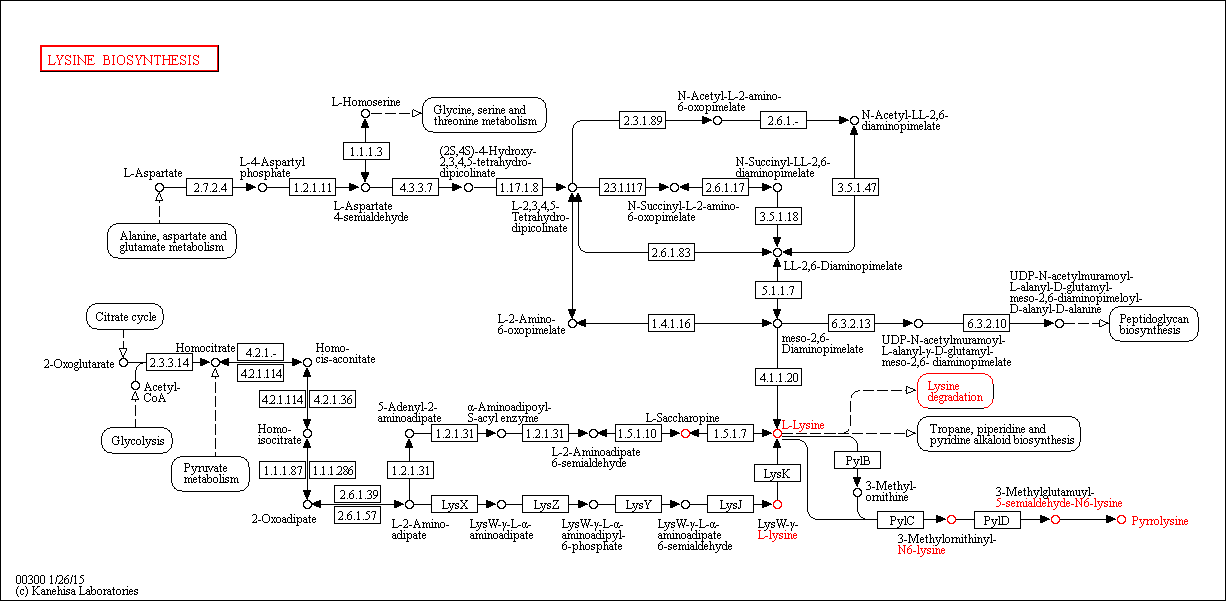
\includegraphics[width=\textwidth]{img/kegg_lysine.png}
        \caption{ Représentation du réseau métabolique selon un graphe dirigé. Les sommets du graphe sont des métabolites et les arcs correspondent aux réactions. Carte extraite de la ressource en ligne "KEGG pathway". }
        \label{fig:kegg_lysine}
    \end{shadedfigure}
    
    \subsubsection{Reactome}
    Le projet Reactome \cite{joshi2005reactome,matthews2009reactome,croft2010reactome,croft2014reactome,fabregat2016reactome} met à la disposition de la communauté des voies métaboliques expertisées et vérifiées par l'Homme. Différentes vues sont proposées selon le niveau hiérarchique du concept sélectionné (voir \cref{fig:reactome_metabolism} et \cref{fig:reactome_serine}). Cette ressource contient à ce jour dix-neuf organismes eucaryotes dont l’Homme. La curation, puis l'organisation des données, est couteuse en temps. Pour donner un ordre d'idée sur l'avancement du travail d'expertise et d'intégration, la version 54 de septembre 2015 comprenait 43\% des gènes humains. Ceci représente un total de 8701 gènes sur les 20 000 gènes codant des protéines.
    
    \begin{shadedfigure}[H]
        \begin{subfigure}[t]{.5\textwidth}
            \centering
            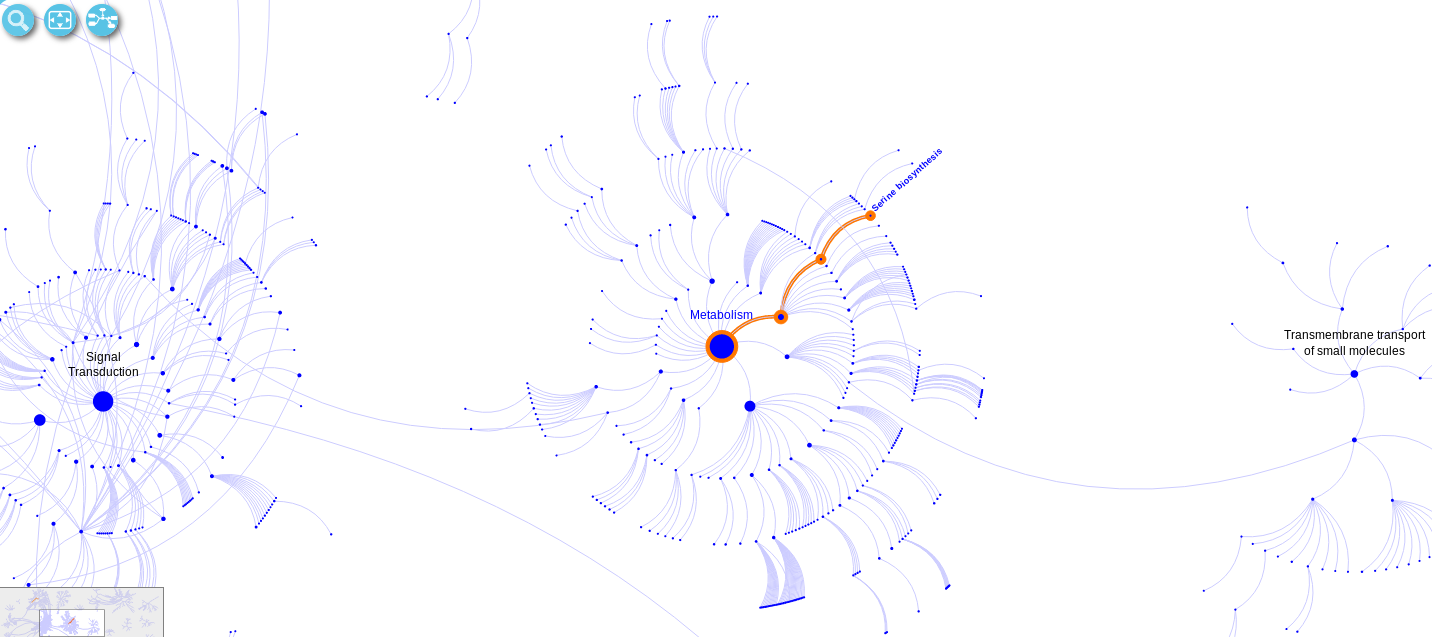
\includegraphics[angle=90,origin=c,width=\textwidth]{img/reactome_homo_sapiens_metabolism.png}
            \caption{ Vue globale des relations ontologique chez l'Homme sous forme de graphe. En naviguant du centre vers l'extrémité des sous-graphes, les concepts vont des plus généraux aux plus spécifiques. }
            \label{fig:reactome_metabolism}
        \end{subfigure}
    \hfill
    \begin{subfigure}[t]{.45\textwidth}
        \centering
        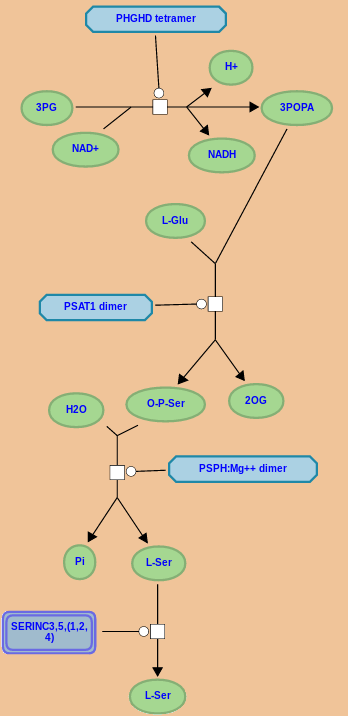
\includegraphics[width=\textwidth]{img/reactome_homo_sapiens_serine_biosynthesis.png}
        \caption{ Représentation du réseau métabolique selon un hypergraphe dirigé. Les sommets verts sont les métabolites et cofacteurs participant à la réaction. Les réactions correspondent aux sommets représentés par des carrés blancs. Les sommets cerclés de bleu sont les étiquettes attachées à la réaction, afin d'indiquer le nom de l'enzyme, le numéro \acrfull{EC} de la réaction et autres informations\ldots. Les hyper-arêtes indiquent le sens de la réaction et pointes sur les molécules transformées. }
        \label{fig:reactome_serine}
    \end{subfigure}
    \end{shadedfigure}

    \subsubsection{UniPathway}
    
    Cette ressource en ligne proposait des voies métaboliques validées par des bio-curateurs de l’institut suisse de bio-informatique \cite{morgat2011unipathway}. Dans cette ressource, le réseau métabolique est décomposé en cinq concepts : les voies métaboliques (\acrfull{UPA}), les chemins réactionnels linéaires (\acrfull{ULS}), les réactions enzymatiques (\acrfull{UER}), les réactions chimiques (\acrfull{UCR}) , les composés (\acrfull{UPC}) (voir \cref{fig:unipathway_structure}). Ces concepts sont ordonnés les uns par rapport aux autres \textit{via} des relations de composition et d'équivalence. Le modèle est très complet : il fait une distinction entre réaction chimique et réaction enzymatique. En effet une réaction chimique peut être spontanée et/ou être réalisée par différentes activités enzymatiques. Inversement, une réaction/activité enzymatique peut réaliser plusieurs transformations chimiques. Enfin à travers le concept d'\acrfull{ULS}, la ressource fait apparaître les enchaînements de réactions permettant de réaliser un objectif biologique. Un \acrfull{ULS} est un ensemble de réactions (\acrfull{UER}) impliqué dans une  tâche biologique unique. Ainsi les \acrfull{ULS} comprenant plusieurs réactions sont délimitées par des réactions impliquées dans au moins deux processus biologiques. Cependant, il est très fréquent de voir une même réaction impliquée dans plusieurs processus biologiques. C'est pourquoi seulement 30\% des \acrfull{ULS} ont plus de deux réactions.
    
    
    \begin{shadedfigure}[H]
        \centering
        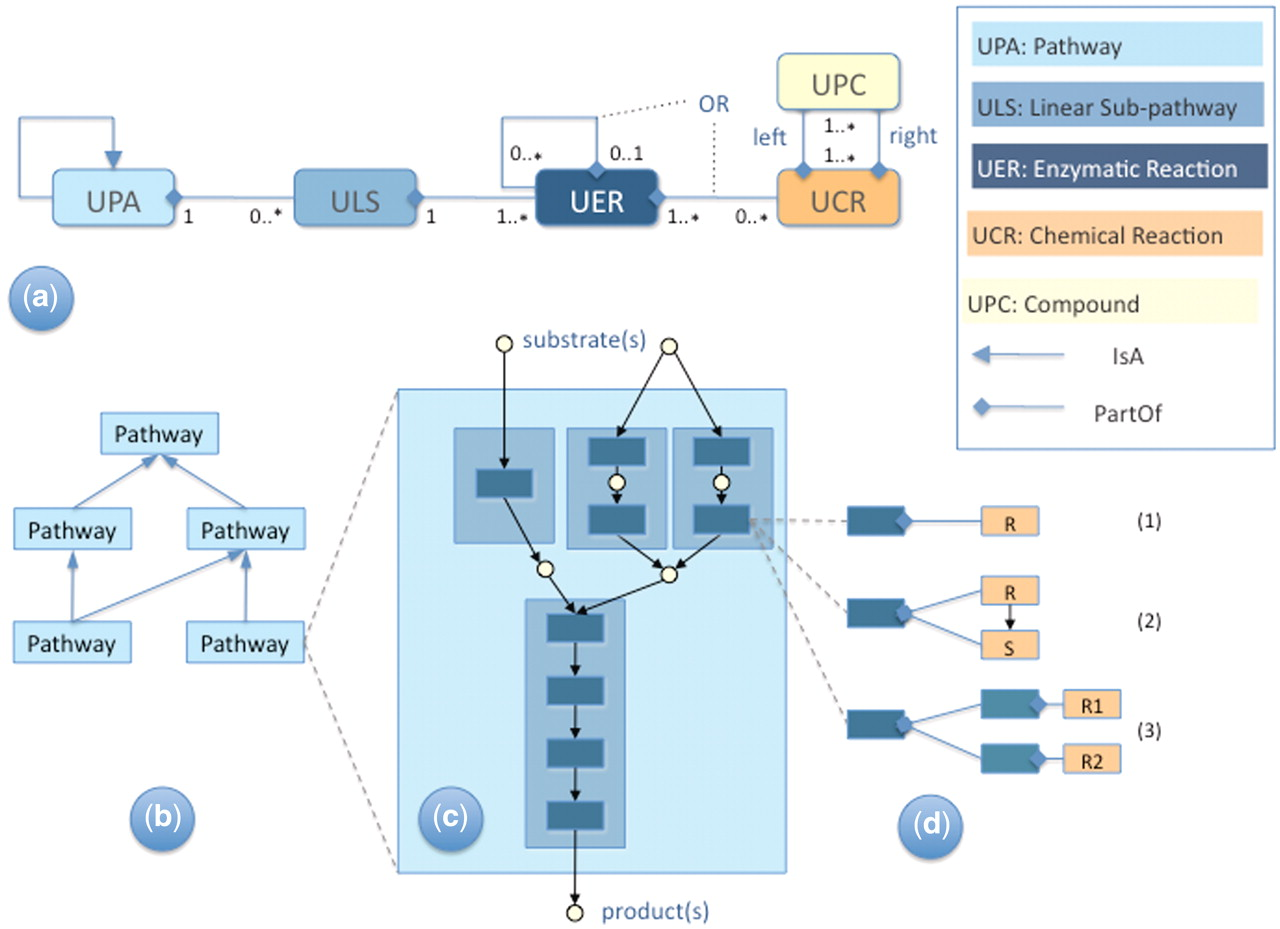
\includegraphics[width=\textwidth]{img/unipathway_structure.jpeg}
        \caption{ Overview of the UniPathway concepts. (a) Unified Modeling Language (UML)-like representation of the UniPathway classes and relationships. Legend is to the right of the main part of the figure. Multiplicity constraints read as: One UPA is composed of 0 or more ULS—One ULS is contained in exactly 1 UPA. One ULS is composed of 1 or more UER—One UER is contained in exactly 1 ULS. One UER is composed of 0 or more (alternate) UER—One UER is contained in 0 or at most 1 UER. One UER is composed of 0 or more UCR—One UCR is contained in 1 or more UER. One UCR is composed of 1 or more left UPC and 1 or more right UPC—One UPC is contained in 1 or more UCR. (b) Example of the IsA relationship defining the UniPathway controlled vocabulary hierarchy of pathway terms. A pathway instance may be a specific type of an abstract pathway entity. (c) Example of the PartOf relationship linking a pathway (UPA: light blue), its subpathways (ULS: blue) and individual enzymatic reactions that constitute the subpathway (UER: dark blue). (d) Three cases of the relationship between an UER and its chemical reaction components (UCR): (1) simple one-to-one relationship where R is catalyzed by a single enzyme; (2) R is catalyzed by an enzyme and S is a spontaneous reaction; (3) ‘OR’ relationship: the enzyme can catalyze two reactions differing by their co-substrates (e.g. NADH/NADPH).}
        \label{fig:unipathway_structure}
    \end{shadedfigure}

    \subsubsection{BioCyc et MetaCyc}
    
    \texttt{BioCyc} \cite{caspi2006metacyc,caspi2007metacyc,caspi2008metacyc,caspi2010metacyc,caspi2012metacyc,caspi2013metacyc,caspi2014metacyc,caspi2015metacyc,caspi2016metacyc} est une collection de base de données génomiques et métaboliques (dénotées PGDBs pour "Pathway/Genome DataBases") avec en plus des outils bio-informatiques pour l'analyse de ces données. Cette ressource en ligne (\url{https://biocyc.org/}) fournit des données de qualité à travers une structure multi-couche afin d'avoir un panel d'information large et cohérent (voir \cref{fig:biocyc_collection}) . Ajouté à ces données biologiques, BioCyc dispose d'un logiciel pour la compréhension des systèmes biologiques nommé  "\texttt{PathwayTools}"\footnote{\url{https://biocyc.org/intro.shtml}}\footnote{\url{http://bioinformatics.ai.sri.com/ptools/}} \cite{karpe2011pathway,karp2015pathway}. Il est composé de quatre composants afin de couvrir un large éventail de cas d'utilisation. Le premier composant s'appelle "\texttt{PathoLogic}", il est utilisé pour créer les PGDBs de tiers 2 et 3. Les voies métaboliques issues de cet outil sont des prédictions portant sur un organisme. Ce composant identifie également les opérons \cite{romero2004using} et suggère des gènes pour les enzymes orphelines\footnote{Une activité enzymatique est dite orpheline lorsque l'on n'est pas capable de l'associer à un gène.}\cite{Green2004}. Le deuxième composant "Pathway/Genome Navigator" permet la visualisation et l'exploration des PGDBs. Il dispose également d'un système d'interrogation de PGDBs. Le troisième composant se nomme "\texttt{MetaFlux}", il est utilisé pour développer des modèles de flux métaboliques. Quant au dernier composant "Pathway/Genome Editors", il permet aux utilisateurs d'éditer les PGDBs. Ce composant est utilisé principalement par les curateurs pour les PGDBs de tiers 1. \textit{BioCyc} intègre également les informations d'autres bases de données de bio-informatique, telles que les caractéristiques des protéines et l'information ontologique d'\texttt{UniProt} . Le site Web \texttt{BioCyc} offre une suite d'outils logiciels pour la recherche, l'analyse et la visualisation de données métaboliques.
    
    
    \begin{shadedfigure}[H]
    	\centering
    	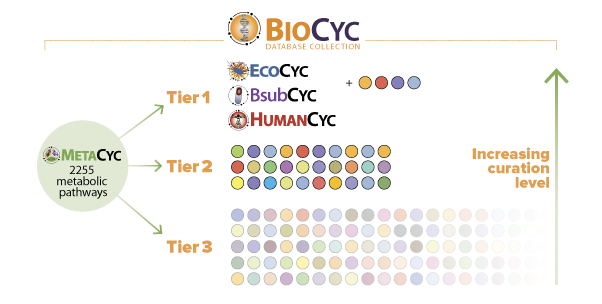
\includegraphics[width=\textwidth]{img/BioCycCollection.png}
    	\caption{\texttt{BioCyc} est un ensemble de bases de données et d'outils sur le métabolisme. \texttt{Metacyc} regroupe l'ensemble des informations du monde vivant. Cette ressource comprend 2255 voies métaboliques à ce jour. Ces données biologiques sont réparties à travers 3 couches (i.e "Tiers"). Ces couches classifient le niveau de qualité des bases de données  (Du moins vers le plus qualitatif : tiers 3 à 1). \hspace{\textwidth} Source : \url{https://biocyc.org/}    }
    	\label{fig:biocyc_collection}
    \end{shadedfigure}
    
    \textit{MetaCyc} \cite{Karp2011,caspi2013metacyc,caspi2016metacyc} est une ressource universelle non redondante sur les voies métaboliques et les enzymes de tous les domaines du vivant. Cette ressource fournit des informations de qualité. Pour cela, elle intègre seulement les voies métaboliques décrite dans la littérature scientifique et expérimentalement observées. Au sein du projet \textit{BioCyc} cette base de données est utilisée conjointement avec la partie \texttt{PathoLogic} de l'outil \texttt{PathwayTools} pour la prédiction de voies métaboliques de tout organisme complètement séquencé (PGDBs).  
    
    À travers les bases de données spécialisées sur un organisme comme \texttt{EcoCyc} (\url{https://ecocyc.org/}) pour \textit{Escherichia coli}, \texttt{BsubCyc} (\url{https://bsubcyc.org/}) pour \textit{Bacillus subtilis} ou encore \texttt{HumanCyc} (\url{https://humancyc.org/}) pour l'Homme, \texttt{BioCyc} fournit une vue précise des informations sur l'organisme d'intérêt. Ces sites spécialisés sont utiles pour faire un bilan des connaissances accumulées au sein d'une espèce. Pour cela des outils dédiés viennent enrichir l'expérience utilisateur, comme la navigation dans le génome avec les annotations fonctionnelles sur les gènes (\url{https://ecocyc.org/ECOLI/select-gen-el}). On retrouve également une carte métabolique offrant une vue globale des connaissances métaboliques sur l'organisme (voir \url{https://bsubcyc.org/overviewsWeb/celOv.shtml} ). Ces données spécialisées peuvent être comparées aux autres organismes  (voir \url{https://humancyc.org/comp-genomics}) afin de mettre en évidence des connaissances communes (voir \cref{tab:compare_tools}).
    
    \begin{table}[H]
    	\caption{Extrait d'une analyse comparative sur les voies métaboliques communes entre d'\textit{Escherechia coli K-12 substr. MG1655}, \textit{Salmonella enterica enterica serovar Typhi str. CT18} et \textit{Shigella dysenteriae 1012} (requête: \url{https://ecocyc.org/comp-genomics?tables=pathway&orgids=\%28ECOLI+SENT220341+SDYS358708\%29}). }
    	\label{tab:compare_tools} 
    	\begin{tabular}{l|lll}
    		\toprule
    		Pathways Shared by Organism Pairs & Escherichia & Salmonella & Shigella \\
    		\midrule
    		Escherichia                       & 342         & 212        & 219      \\           
    		Salmonella                        & 212         & 341        & 274      \\           
    		Shigella                          & 219         & 274        & 335      \\ 
    		\bottomrule
    	\end{tabular}
    \end{table}
    
    
    Toutes ces données spécialisées sont croisées pour produire de la connaissance. Afin de visualiser ces connaissances \textit{Biocyc} met à disposition des tables de connaissances interactives, les "\acrfull{KS}" \cite{bat061SmartTable}. Ces tables intelligentes utilisent la représentation symbolique des connaissances. Elles permettent de regrouper les connaissances vis-à-vis de leur signification. Par exemple, le groupe des "composés anti-tuberculose  et leurs cibles dans  \textit{Mycobacterium tuberculosis} H37Rv" est formé par l'analyse sémantique des données (voir le groupe : \url{https://biocyc.org/group?id=biocyc14-1553-3679321317}).
    
    La représentation des voies métaboliques est découpé par chemin de réaction (appelé également variant) pour atteindre un objectif biologique. ci-a près une des six voies alternatives pour la biosynthèse de la lysine ( \cref{fig:metacyc_lysine}  ).
    
    \begin{shadedfigure}[H]
        \centering
        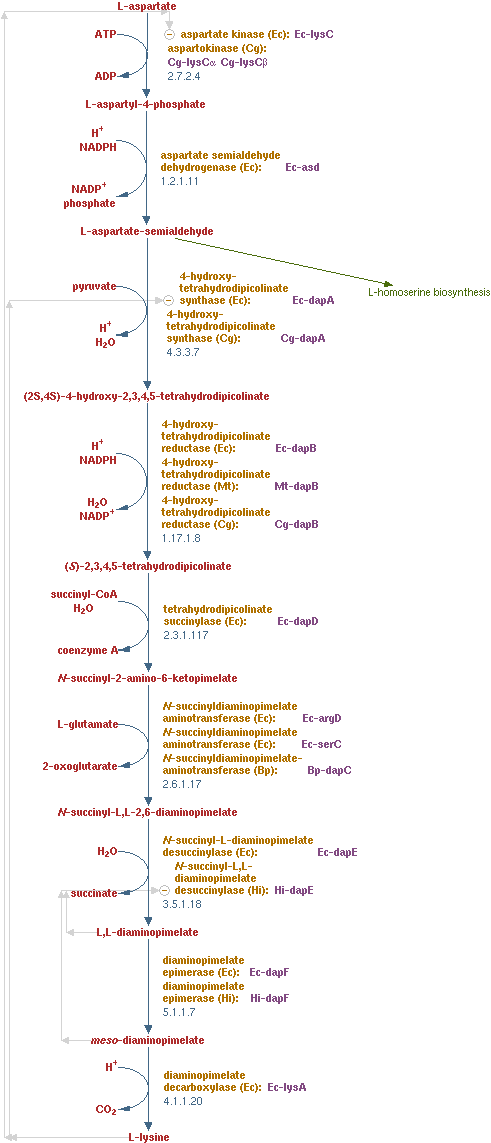
\includegraphics[height=0.8\textheight]{img/lysine_biosynthesis_1_metacyc.png}
        \caption{Représentation d'un variant de la biosynthèse de la lysine, dénommé: L-lysine biosynthesis I }
        \label{fig:metacyc_lysine}
    \end{shadedfigure}
    
    
    \section{Des génomes aux réseaux métaboliques}
    
    Le génome d'un organisme contient l'information pour produire des protéines \ref{fig:production_proteine}. Ce génome est constitué d'\gls{ADN} dont l'ordonnancement de ces bases ont une signification biologique. Par analogie, comprendre l'information dans le génome c'est comme lire un livre de cuisine composé uniquement de quatre lettres (ACGT: adénine, cytosine, guanine, thymine) et décrivant seulement la liste des ingrédients pour chaque recette. Cette petite digression fait référence aux gènes, ce sont des suites de nucléotides décrivant la composition et l'ordre en acide aminé d'une protéine. Pour cela, la séquence d'\gls{ADN} d'un gène est transcrite en \gls{ARNm}. Puis la séquence d'{ARNm} est traduit en une protéine.
     
    La connaissance de tous les gènes permet d'avoir un catalogue des capacités du vivant dans, notamment, le métabolisme. Cette longue tâche d'inventaire et de mise en relation des gènes/protéines/réactions est rentabilisée par la réutilisation de ces connaissances pour d'autres organismes. En effet, la recherche d'une fonction biologique peut se faire par la suite dans tous les organismes par homologie de séquence protéique. Afin d'aborder les liens entre le génome et le métabolisme d'un organisme, nous rappelons brièvement les trois niveaux qui les relient. Ceci implique :\nolisttopbreak
    
    \begin{itemize}
        \item Le génome : composé d'un ensemble de gènes
        \item Le transcriptome : constitué d'\gls{ARN} produit par l'organisme
        \item Le protéome : ensemble des protéines exprimées par l'organisme
    \end{itemize}

\note{La séquence \gls{ADN} peut être vue comme un support de stockage décrivant la composition des protéines. D'ailleurs des chercheurs travaillent sur la mise au point de méthodes pour lire et écrire des données dans une séquence d'\gls{ADN} \cite{bornholt2016dna,yazdi2015rewritable}. Ils estiment qu'une telle séquence peut stocker 87,5 TeraBytes de données par gramme. Par comparaison un disque dur classique d'1TB pèse environ 100 gramme. Une telle prouesse révolutionnerais les systèmes d'archivages.}
    
    \begin{shadedfigure}[H]
        \centering
        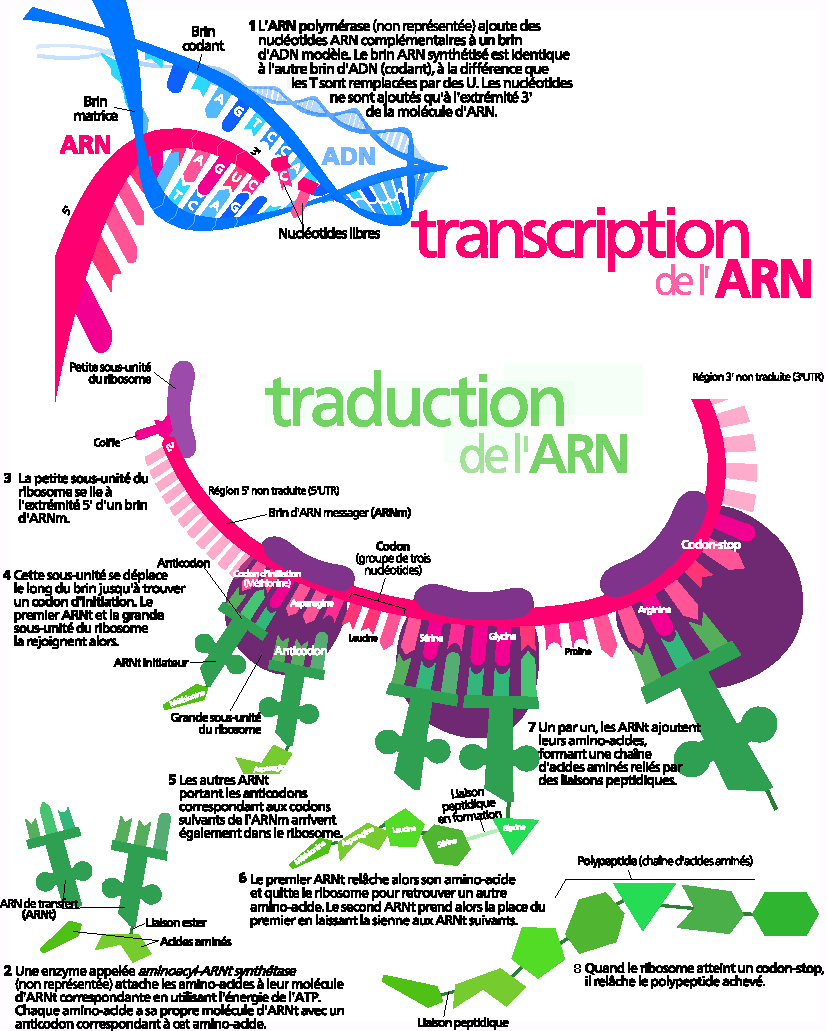
\includegraphics[width=\textwidth]{img/production_proteine2.pdf}
        \caption{Schéma des différentes étapes aboutissant à la production d’une protéine.}
        \label{fig:production_proteine}
    \end{shadedfigure}
    
    Le transcriptome et dans un second temps le protéome représentent les produits de l'expression des gènes. Ces deux niveaux sont dynamiques et changeant. Ils diffèrent selon les stress perçus par l'organisme. C'est-à-dire, à un temps donné, seulement une partie des gènes de l'organisme est exprimée. Ainsi pour chaque gène retrouvé dans un organisme, on sera en mesure de déterminer la ou les séquence(s) protéique(s) \footnote{Un même gène peut exprimer plusieurs protéines.}. Le lien indirect entre les gènes, les protéines et les réactions est également appelé "\acrshort{GPR}" pour : \textit{\acrfull{GPR}}.
    
    \subsection{L’évolution des génomes}
    Avant d'approfondir l’annotation génomique, il est nécessaire de comprendre le processus d’évolution des génomes. En effet les méthodes d’annotation automatique utilisent en partie cette théorie pour extrapoler des fonctionnalités d’un organisme vers un autre.
    
    Le principe de l'évolution explique que le vivant est soumis à différentes contraintes, environnementales par exemple ( ressources nutritives, température, acidité\ldots ). Ainsi avec le temps, les générations d’individus les plus adaptées à ces contraintes ont de meilleurs chances de se reproduire et par conséquent de transmettre leur patrimoine génétique. D’ailleurs c’est ce patrimoine génétique qui permet de s’adapter aux contraintes environnementales. Il est notamment le support de l’expression métabolique et ce métabolisme peut fournir des avantages à un individu par rapport aux autres. Ainsi, tant que le métabolisme d’un organisme est adapté à ces contraintes, l’individu peut se reproduire et perpétuer sa lignée.
    
    En effet, différents événements de mutation (changement de nucléotides), de duplication ou d’acquisition d’ADN exogène (transfert horizontal) peuvent le modifier le génome. Par conséquent les gènes modifiés ou acquis vont produire des protéines différentes. Ces modifications peuvent alors procurer soit un avantage soit un désavantage qui va mener à la fin de la transmission de ce patrimoine. C'est la raison pour laquelle, nous observons la plupart du temps seulement les organismes possédant un patrimoine génétique suffisamment adapté à leurs contraintes environnementales. En bref, les organismes et leurs gènes sous l’effet de pressions variées sont sélectionnés.
    
    Pour cette raison, les gènes de fonction similaire ont souvent un ancêtre commun\footnote{Il existe d'autre cas comme la convergence évolutive qui amène également à des protéines de fonctions similaires. } . Ce qui nous permet d'introduire la notion d'homologie. Ce terme est utilisé pour décrire deux gènes qui ont dérivé d'un ancêtre commun. L'homologie n'est pas quantifiable, pour cela on invoquera plutôt la notion de similarité de séquence. Cette notion permet de comparer par alignement deux séquences (homologues ou non) et d'informer dans quelle proportion elles disposent de régions communes. Par contraste, les gènes d’organismes différents n’ayant pas la même origine évolutive sont définis comme analogues. La notion d'orthologie est utilisée pour définir des séquences homologues qui proviennent d’un gène unique présent dans le dernier ancêtre commun. Pour décrire des gènes homologues issus d'événements de duplication au sein d'un génome ou dans les génomes ancestraux, on parle de paralogie. De tels événement peuvent dupliquer un gène, une région de génome contenant plusieurs gènes voir dans certains cas un génome entier.
    
    \begin{shadedfigure}[H]
        \centering
        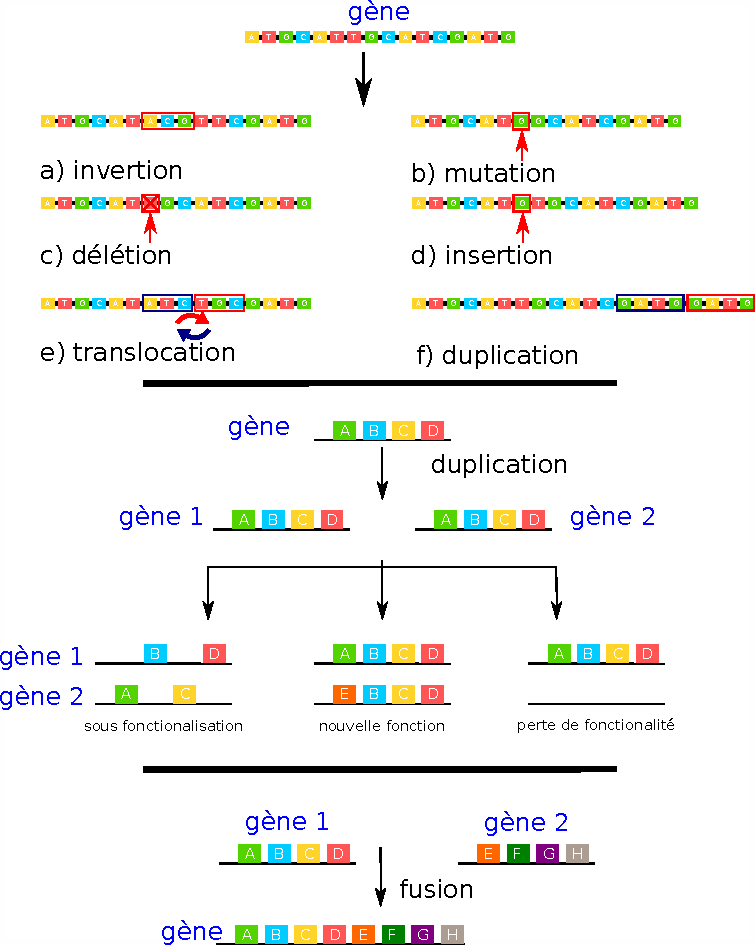
\includegraphics[width=\textwidth]{img/gene_indel.pdf}
        \caption{Présentation de plusieurs événements génomiques....}
        \label{fig:/evenement_mutation}
    \end{shadedfigure}
    
    
    Un événement de duplication de gène génère une nouvelle copie de gène dans l’organisme. Étant donné que l'organisme possède une fonctionnalité en double, une des copies peut diverger en terme de fonction par l’acquisition de mutations. 
    
    Les événements de fusion de gènes représentent des gènes originellement séparés qui vont former un unique gène. Par opposition, les événements de fission vont  engendrer la coupure d’un gène en deux gènes distincts. Typiquement la fusion est observé avec des gènes codants pour des protéines multi-domaines. Par exemple, deux gènes impliqués dans la traduction de deux domaines distincts d'une protéine fusionnent de telle sorte que ces domaines soient co-exprimés dans un même gène pour, faciliter, par exemple le processus de régulation.
    
    Le relâchement de certains facteurs de pression de sélection peut conduire à des événements de perte de fonction par délétion ou inactivation d’un gène, par exemple, par un événement de fission conduisant à un pseudogène.
    
    On retrouve également des événements d’inversion de séquence, de translocation ou transposition (un ou plusieurs gènes vont changer de région génomique au sein d’un chromosome ou vers un autre chromosome).
    
    L’accumulation de tous ces événements peut amener à une divergence importante du génome par rapport au génome ancestral. Ceci conduit à l’émergence de nouvelle espèces qui vont évoluer différemment. On parle d'événement de spéciation.
    
    La fréquence d'apparition de mutation au sein d'une espèce dans son habitat naturel est relativement constante car soumise aux mêmes mécanismes intra-cellulaires. Partant de ce constat, il existe l'hypothèse de l’horloge moléculaire selon laquelle l'accumulation de mutation dans le génome est constante. Cette horloge est plus rapide sur les régions qui ne sont pas soumises à la pression de sélection naturelle et plus lente dans les parties du génome soumises à une forte pression (c'est-à-dire les régions codant pour des fonctions essentielles à la survie de l'organisme).
    
    
    \subsection{Annotation des génomes}\label{subsec:annotation}
    
    Afin de documenter le génome, le transcriptome et le protéome on passe par plusieurs étapes d’annotation. L’annotation peut être de nature automatique ou manuelle. Dans ce dernier cas, des experts vont effectuer un travail de validation et invalidation des annotations. Ce travail de curation des données est important car les prédicteurs automatiques ne sont pas toujours fiables.
    
    On distingue trois niveaux d’annotation pour un génome (\cref{fig:niveaux_annotation}). Le premier niveau est l’annotation structurale. Elle est utilisée pour définir des régions d’intérêt sur la séquence comme les bornes de début et de fin des gènes.  Le second niveau est l’annotation fonctionnelle. Elle recherche à prédire les fonctions biologiques des gènes. Puis, le troisième niveau correspond à l’annotation relationnelle. Cette annotation consiste à identifier les différentes interactions entre les gènes et leurs produits.
    
    \begin{shadedfigure}[H]
        \centering
        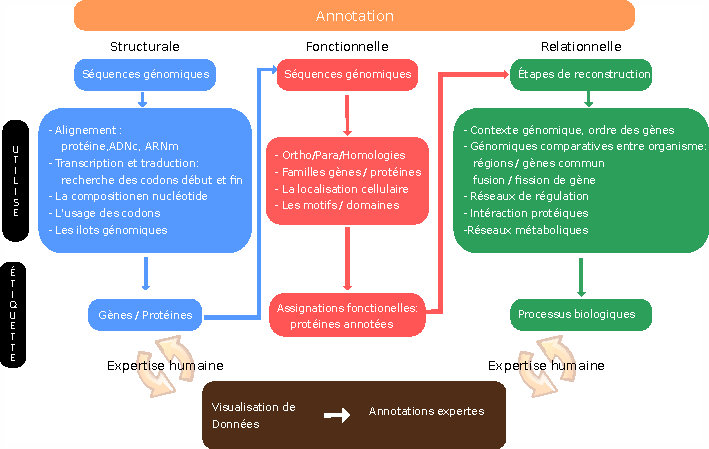
\includegraphics[width=\textwidth]{img/niveaux_annotations.pdf}
        \caption{Présentation des trois niveaux d’annotation. 1) Annotation Structurale : identification des gènes et des séquences issue de transcription et la traduction. 2) Annotation Fonctionnelle : attribution des objectifs biologiques réalisé pars les séquences précédemment identifiées (usuellement par homologie avec une séquence de fonction connue). 3) Annotation Relationnelle : regroupe différentes relations établis entre les séquences pour décrire des objectifs biologiques telle qu'une voie métabolique.  }
        \label{fig:niveaux_annotation}
    \end{shadedfigure}
    
    L’annotation fonctionnelle, correspond au processus d’attribution de rôles biologiques à des gènes. En effet, ces gènes vont produire des protéines disposant d'une ou plusieurs fonctionnalités pour l’organisme. Ces fonctions sont habituellement classées en trois catégories : moléculaires, cellulaires, phénotypiques.
    
    Les fonctions moléculaires décrivent le rôle biochimique et/ou structural de la protéine. Ainsi, les fonctionnalités de catalyse, de liaison et autres sont présentées.
    
    Les fonctions cellulaires établissent les différentes interactions de la protéines au sein de la cellule. Par exemple, le rôle d’une enzyme dans une voie métabolique comme la biosynthèse de la lysine . 
    
    Les fonctions phénotypiques détaillent les caractéristiques observables induite par l’activité d’une ou plusieurs protéines. À titre d’exemple, la présence ou l’absence d’une protéine peut jouer un rôle sur la capacité de l’organisme à se développer dans un environnement.
    
    L’annotation fonctionnelle peut être basée sur des méthodes expérimentales. Par exemple, un gène peut être cloné dans un vecteur d’expression pour produire la protéine correspondante dans un autre organisme facilement manipulable en laboratoire. Cette expression hétérologue permet ensuite de purifier la protéine et de tester, par exemple, son activité biochimique dans le cas d’une enzyme. Ces méthodes expérimentales ne sont  pas envisageables pour caractériser la fonction de tous les gènes  d’un organisme car elles demandent beaucoup de temps de conception et de réalisation.
    
    Les méthodes d’annotation bio-informatiques fonctionnelles  bio-informatiques se basent sur la comparaison de séquences. Ainsi, les séquences homologues, les protéines d'une même famille, les séquences possédant un domaine ou un motif peuvent partager des annotations fonctionnelles.
    
    \subsection{Reconstruction des réseaux métaboliques}
    Le métabolisme est un ensemble de réactions biochimiques. Une réaction transforme des composés en de nouveaux métabolites. Ces derniers sont modifiés par d'autres transformations. Cette succession d'événements peut être représentée sous la forme d’un graphe de réactions. Le produit d’une réaction est relié à une autre réaction lorsque cette dernière utilise ce métabolite transformé.
    
    
    \begin{shadedfigure}[H]
        \centering
        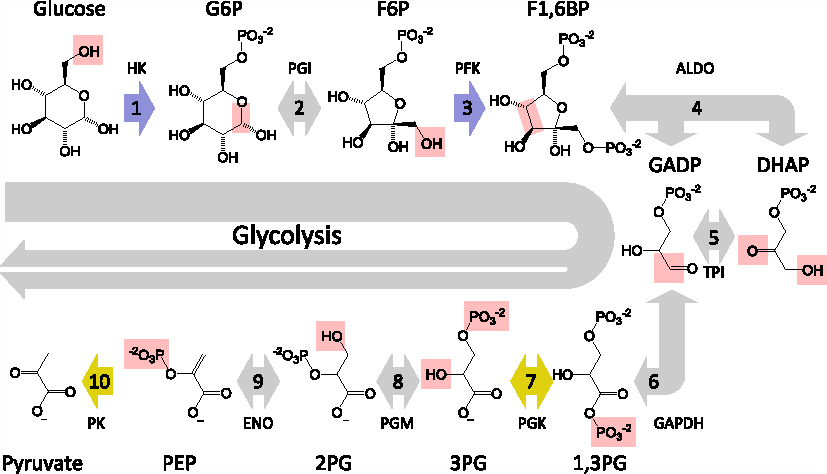
\includegraphics[width=\textwidth]{img/graphe_reactions_glycolyse.pdf}
%        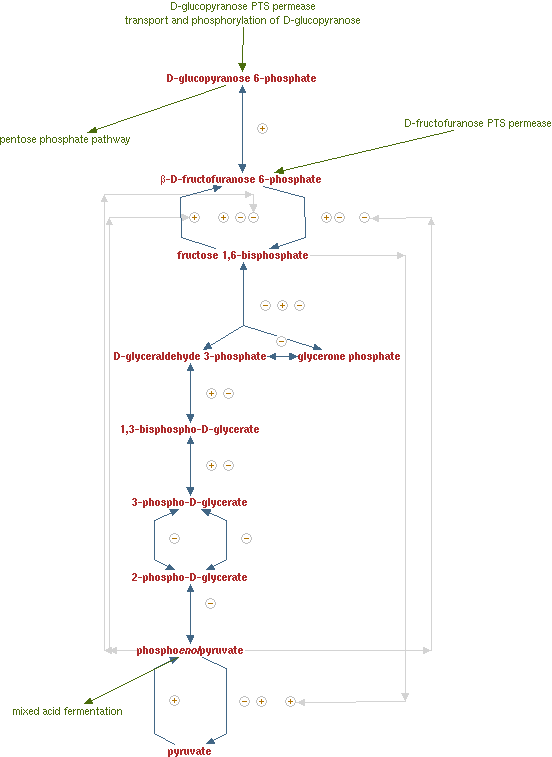
\includegraphics[width=\textwidth]{img/glycolysis.png}
        \caption{Représentation de la dégradation du glucose sous forme d’un graphe réactionnel. La  succession des réactions forme un chemin dans le réseau. Cette représentation a pour vocation de restreindre les événements qui occurrent dans l'organisme aux réactions. Il est important de retenir que ce type de schéma, n'indique pas si ces réactions ont lieu dans le même compartiment cellulaire. Ou encore si les protéines nécessaires aux réactions sont toutes présentes à un moment donné. Cette une vue générale des réactions pouvant avoir lieu dans un organisme. \hspace{\textwidth}\tiny{Source: \url{https://en.wikipedia.org/wiki/Glycolysis}}  }
        \label{fig:glycolysis}
    \end{shadedfigure}

    \subsection{Les données expérimentales}
    
    \subsubsection{Élucidation des voies métaboliques}
    Avec la découverte des enzymes à la fin du \siecle{19}, un nouveau champ de connaissance en biologie s’ouvrait. L’enzyme est la clé menant à la compréhension du vivant. Pour cela, la communauté scientifique réalisa un très grand nombre d’expériences permettant produire puis ...
    \subsubsection{Phénotypes de croissances}
    La plupart des molécules biologiques sont constituées d’atome de  carbone (C), d’hydrogène (H), d’oxygène (O), d’azote (N), de phosphore (P) et de soufre (S) (\acrshort{CHONPS}). Par conséquent les organismes doivent avoir au moins une source de nutrition pour chacun de ces éléments. En plus de ces éléments, on considère qu’il est nécessaire pour la vie d’avoir une source de potassium, de calcium, de magnésium, de fer, d’oligo-éléments et d’eau. Ce sont les éléments minimum pour la vie. Tout autre élément permettant à des organismes de se développer est catégorisé comme facteur de croissance. 
    
    Selon les organismes vivants, leurs besoins en éléments et facteurs de croissances varient avec leur capacité métabolique. Ce qui permet de catégoriser les organismes, au regard des manières de constituer de la matière organique via leur anabolisme, ainsi que des moyens de production énergétique via leur catabolisme. (trop lourd) Ces catégories dites types trophiques dépendent de la nature  (i) de la source de carbone (ii) du donneur d’électrons (iii) de la source d'énergie (voir \cref{tab:type trophique}).
    \begin{landscape}
        \begin{table}[H]
            \centering
            \caption{Structuration des différents types trophiques.}
            \label{tab:type trophique}
            \begin{tabular}{|l|l|lr|l|}
            	\hline
                \multirow{2}{*}{\specialcell{Lumière\\\textcolor{orange}{Photo}-}}    					      	&  \multirow{2}{*}{\specialcell{Composé organique\\-\textcolor{nicered}{organo}-}}  & Organique & -\textcolor{psviolet}{hétérotrophe} 	& \textcolor{orange}{Photo}\textcolor{nicered}{organo}\textcolor{psviolet}{hétérotrophe}    \\\cline{3-5}
                                                                                          					  	&                                                               					& Minérale 	& -\textcolor{bleudefrance}{autotrophe}	& \textcolor{orange}{Photo}\textcolor{nicered}{organo}\textcolor{bleudefrance}{autotrophe}  \\\cline{2-5}
                                                                                         					   	&  \multirow{2}{*}{\specialcell{Inorganique\\-\textcolor{brown}{litho}-}}           & Organique & -\textcolor{psviolet}{hétérotrophe} 	& \textcolor{orange}{Photo}\textcolor{brown}{litho}\textcolor{psviolet}{hétérotrophe}     	\\\cline{3-5}
                                                                                            					&                                                               					& Minérale 	& -\textcolor{bleudefrance}{autotrophe}	& \textcolor{orange}{Photo}\textcolor{brown}{litho}\textcolor{bleudefrance}{autotrophe}     \\ \hline
                \multirow{2}{*}{\specialcell{Composé chimique\\organique ou non\\\textcolor{vert}{Chimio}-}}  	&  \multirow{2}{*}{\specialcell{Composé organique\\-\textcolor{nicered}{organo}-}}  & Organique & -\textcolor{psviolet}{hétérotrophe} 	& \textcolor{vert}{Chimio}\textcolor{nicered}{organo}\textcolor{psviolet}{hétérotrophe}   	\\\cline{3-5}
                                                                                            					&                                                               					& Minérale 	& -\textcolor{bleudefrance}{autotrophe}	& \textcolor{vert}{Chimio}\textcolor{nicered}{organo}\textcolor{bleudefrance}{autotrophe}   \\\cline{2-5} 
                                                                                            					&  \multirow{2}{*}{\specialcell{Inorganique\\-\textcolor{brown}{litho}-}}           & Organique & -\textcolor{psviolet}{hétérotrophe} 	& \textcolor{vert}{Chimio}\textcolor{brown}{litho}\textcolor{psviolet}{hétérotrophe}    	\\\cline{3-5}
                                                                                            					&                                                               					& Minérale 	& -\textcolor{bleudefrance}{autotrophe}	& \textcolor{vert}{Chimio}\textcolor{brown}{litho}\textcolor{bleudefrance}{autotrophe}      \\ \hline
            \end{tabular}
        \end{table}
    
    \end{landscape}
    Certains organismes ont la faculté de se développer dans des milieux dépourvu de facteur de croissance. C’est-à-dire, qu'à partir des éléments minimaux nécessaires à la vie, ils sont capables de produire toutes les molécules  indispensables à leurs développements. Ce sont des organismes dit prototrophes.  Dans le cas contraire on parle d’auxotrophie. 
    
    Le métabolisme fournit les acides aminés indispensables à la production de protéines. Ces protéines sont constituées d’acides aminés. Par conséquent l’organisme doit se procurer ces acides aminés soit par des voies de biosynthèses soit directement par nutrition. C’est pour cela qu’avec les organismes prototrophes on s’attend à retrouver toutes les voies de la biosynthèses des acides aminés. Et par opposition un organisme auxotrophe à un acide aminé ne devrait pas avoir la voie de biosynthèse de ce dernier.
    
    Les compétences métaboliques d'une bactérie sont testées en laboratoire dans diverses conditions. Lorsque l'on souhaite déterminer la capacité d'un organisme à dégradé ou non d'un nutriment carboné, on place l'organisme dans un milieu avec pour seul source de carbone le nutriment a tester. Un organisme capable de dégradé le composé va réutilisé ses atomes carbones pour alimenter la machinerie cellulaire. C'est la raison pour laquelle l'organisme ve pouvoir se développer sur le milieux de culture et faire croitre sa population. Ces milieux sont constitués des éléments minimaux (\gls{CHONPS}) pour le développement de la vie. La société Biolog \cite{bochner2009global} a développé une méthodologie pour tester 96 conditions de croissances par plaque. Ce procédé permet de cribler les capacités de dégradation à partir de différentes source de carbones, azotes et phosphores. La croissance ou non de l'organisme permet \textit{in-fine} d'attribuer un phénotype. Le biologiste s'attendra à retrouver les gènes impliqués dans la dégradation des composés testés.
    
    \subsection{MicroScope : une plateforme d’annotation de génomes procaryotes et d’analyse de leur métabolisme}
    
    Chapeau : objectif MicroScope, les différentes publications
    Puis celle de 2017
    Section de la fin : souligner ce qui a été fait en terme de curation pour les bio… mais mieux à faire pour guider les bio dans leur travail de curati=> objectif de ton travail
    
    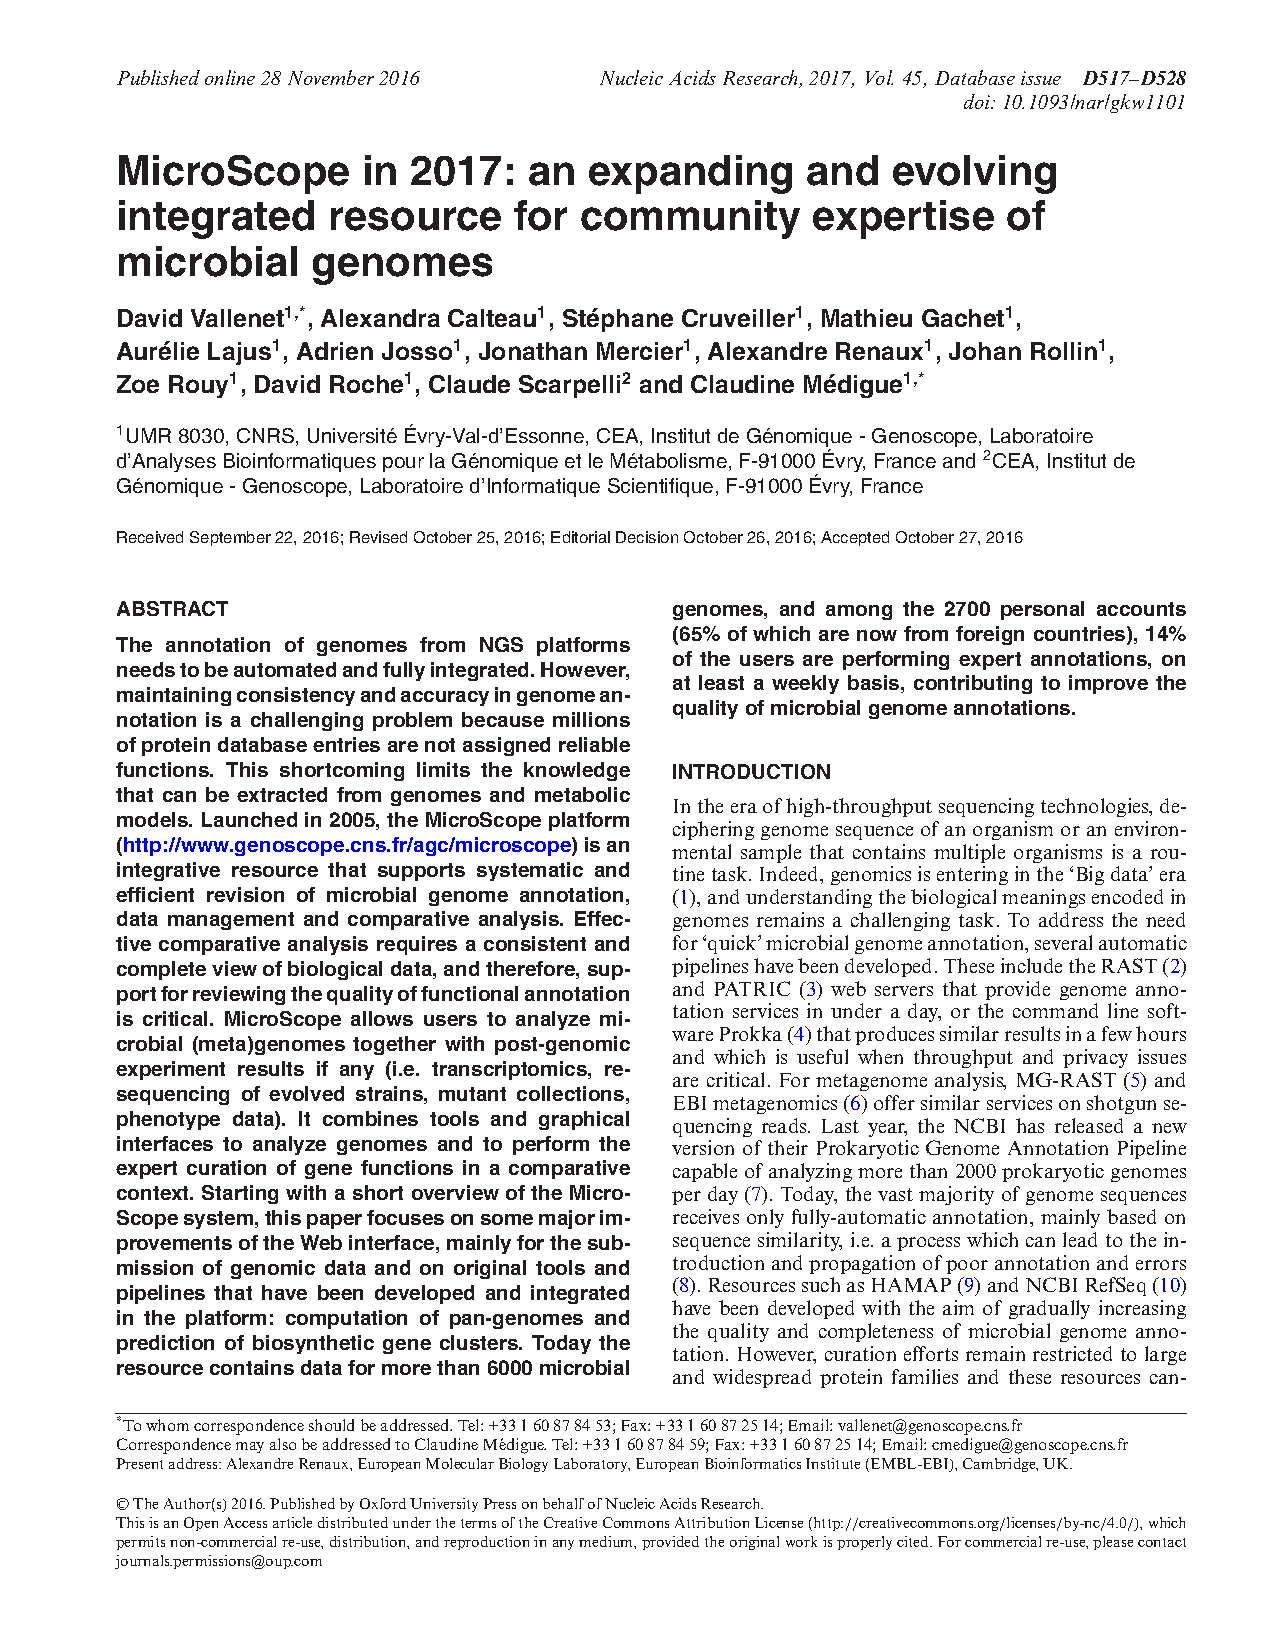
\includepdf[pages=-]{img/microscope2017.pdf}

    \section{Raisonnement logique dans le processus de curation}
    
    Le processus de curation consiste à ajouter, modifier et/ou enlever des annotations produites de façon automatique par les pipelines bio-informatiques (cf. section \cref{subsec:annotation}). Pour cela, les bio-curateurs utilisent des démarches qui leur sont propres et qui peuvent mettre en jeu des règles issues de la connaissance biologique du domaine. Une des méthodes souvent utilisée passe par la reconstruction des voies métaboliques. Le bio-curateur connaît des caractéristiques phénotypiques de son organisme d’intérêt. Il va donc commencer par vérifier si ces caractéristiques sont corrélées aux prédictions. Par exemple, lorsque l’on reconstruit les voies métaboliques de la bactérie \textit{Citrobacter}, parmi les voies métaboliques complètes, on s’attend à retrouver la voie de dégradation du citrate. Si certaines réactions de la voie ne sont pas prédites, le bio-curateur va rechercher un ou plusieurs gènes candidats codant des protéines catalysant ces réactions.
    
    Ce processus de curation réalisé par les biologistes suit un certain raisonnement "logique" qui peut potentiellement être formalisé puis automatisé dans un système informatique.
    
    \subsection{Lacunes et incertitudes dans nos connaissances}\label{subsec:lacunes}
    
    Quel que soit le domaine d’expertise, certains éléments restent imprédictibles par les modèles scientifiques car notre savoir sur le monde qui nous entoure est encore partiel. Les modèles scientifiques permettent de représenter une partie de ce monde. Mais il existe un nombre de faits, non négligeable, qui échappe à ces  modèles. Ces "trous" de connaissances ou lacunes peuvent être identifiés lorsque l’on oppose les prédictions aux expectations qui sont des faits attendues reste mais pas forcément prédits.
    
    \subsubsection{La sur-prédiction}
    
    Les ressources qui entreposent des faits prédits sont variées car ils proviennent de différentes méthodes dont la spécificité \footnote{Proportion de résultats négatifs correctement identifiés.} et la sensibilités \footnote{Proportion de résultats positifs correctement identifiés.} diffèrent selon l’algorithme sous-jacent. Ces prédictions viennent enrichir les entrepôts de données et seront utilisées à leur tour pour prédire de nouveaux faits. Ce processus cyclique permet de capturer un nombre plus important de faits, mais il a potentiellement l’inconvénient de sur-prédire. En effet, le taux d’erreur de la première prédiction vient s’ajouter au taux d’erreur de la prédiction suivante. Ce problème de sur-prédiction peut amener faussement à la prédiction d'une voie métabolique. Pour pallier ce phénomène, des initiatives tentent de limiter l’extrapolation abusive faite par les prédicteurs. Par exemple \citeauthor{pfeiffer2015manual}
    
    
    \subsubsection{Les enzymes orphelines}
    
    Nos connaissances des systèmes biologiques et encore aujourd'hui incomplète. Lorsque l'on regarde de plus près ces lacunes , on remarque que deux éléments semble être liée. Le premier est le grand nombre de gènes de fonction inconnue. Le second part du constat qu'une proportion non négligeable des activités enzymatiques ne sont pas représenté par une enzyme. Dans de tel cas, l'activité enzymatique est "orpheline" de séquence. Elle est qualifiée par la communauté scientifique "d'orphan enzyme" \cite{lespinet2005orphan}. Dans ce contexte, nous ne sommes pas en mesure d'associer une protéine correspondant à l'activité enzymatique observé. Des initiatives comme celle de \citeauthor{karp2004call} tente de mettre en relation au moins une enzyme pour chaque activité enzymatique biochimiquement caractérisée \cite{karp2004call}. La combinaison des résultats expérimentaux et bio-informatiques permet de valider les prédictions et dans certains cas d'identifier l'enzyme. Pour ce faire les méthodes expérimentales doivent pouvoir tester un large spectre de candidat. L'approches expérimentales mises au point par \citeauthor{kuznetsova2005enzyme} a permis d'assigner une fonction catalytique à 36 protéines sur un éventail d'une centaine de protéine tester \cite{kuznetsova2005enzyme}.
    
    Suite à l'appelle de \citeauthor{karp2004call} en 2004, \citeauthor{shearer2014finding} crée le "Orphan Enzyme Project" (\url{http://www.orphanenzymes.org/}). Au début de ce projet plus d'un tiers des 4400 activités enzymatiques décrites par la commission enzymatique (\gls{EC}) était orpheline de séquence. Une approche combinant la bio-informatique et la recherche en laboratoire a permis d'identifier 270 séquences candidate pour une activité orpheline de séquence\cite{shearer2014finding}. Toutefois, les numéros \gls{EC} ne reflètent pas toutes les activités enzymatiques réalisé par le vivant. Lorsque ces activités sont mises en relation avec les voies métaboliques de \texttt{KEGG} et \texttt{MetaCyc}, on dénombre  respectivement 26\% et $39,5$\% d'enzyme orpheline de séquence \cite{sorokina2014profiling}.
    
    \subsubsection{Rôle de la curation}
    
    Afin de réduire les différentes lacunes dans nos connaissances, l'expertise humaine est indispensable. Une fois l'annotation automatique réalisé, les biocurateurs vérifient les fonctions prédites dans l'organisme. Pour cela, la mise en relation des différentes connaissances sur l'organisme permet de trouver des gènes pour les fonctions manquantes et retirer les annotations sur-prédites. Afin de faciliter ce travail de curation des plateformes comme MicroScope \cite{vallenet2016microscope,Belda2017}, \texttt{\gls{IMG}} \cite{markowitz2009img,markowitz2012img} ou encore \texttt{SEED} \cite{overbeek2004seed,overbeek2014seed} fournissent un environnement intégré pour l'annotation des génomes microbien. L'objectif est de collecter et de mettre en relations les informations relatives aux différents gènes identifiés en vue de facilité le travail du curateur. Ainsi le curateur corrige les annotations à travers des interfaces de parcours et d'édition de génome (\cref{fig:edit_microscope}).
    
    \begin{shadedfigure}[H]
        \centering
        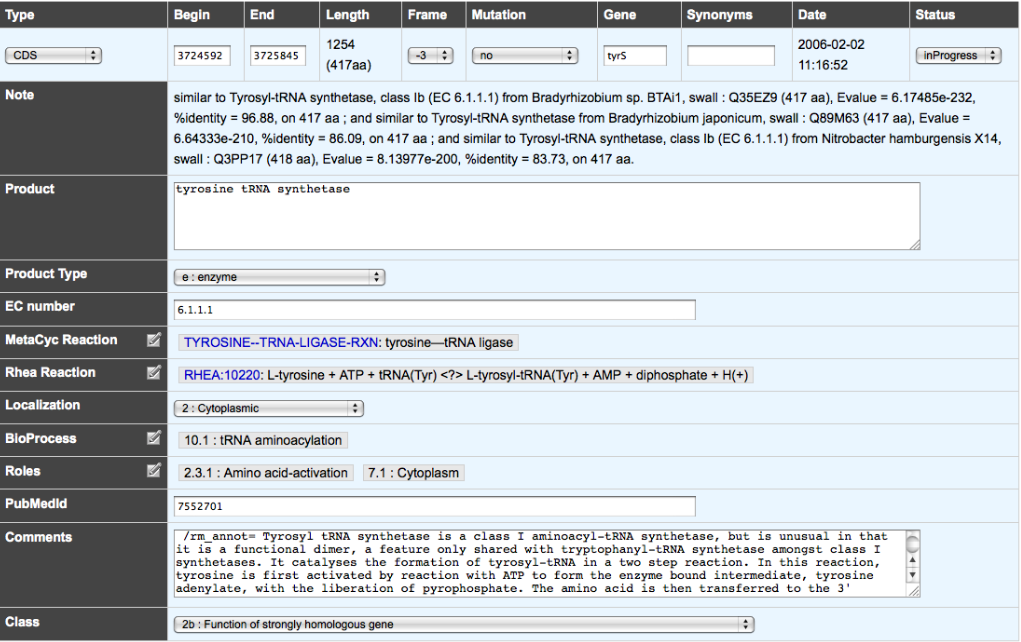
\includegraphics[width=\textwidth]{img/curation_edit.png}
        \caption{Interface d'édition pour l'annotation fonctionnelle des gènes. }
        \label{fig:edit_microscope}
    \end{shadedfigure}
    
    Lors de l'analyse des génomes nouvellement séquencés, le biologiste est confronté à la difficile tâche de vérification de la cohérence des gènes annotés vis-à-vis des connaissances biologiques sur l'organisme étudié. Pour cette raison l'automatisation des règles appliquées par le biologiste permettrais de traiter rapidement une quantité importante d'information.
    
    \subsection{Logique et raisonnement}
    
    La logique est une branche à la fois de la philosophie et des mathématiques. Son utilisation permet, par exemple d'instrumentaliser les mots afin de faire ressortir la vérité d'une phrase. Dès l'Antiquité elle fut employée comme un outil pour distinguer un raisonnement concluant d'un raisonnement non-concluant. \textit{Aristote} formalise une logique à deux énoncés (appelées prémisses ou encore propositions) soumis à approbation. Pour l'illustrer, la phrase suivante: "Tous les hommes sont mortels, or Socrate est un homme donc Socrate est mortel" est constituée de deux prémisses séparées par une virgule et de sa conclusion. Ainsi la vérification de la véracité de ces prémisses conduit à une conclusion pouvant être vraie ou fausse. Cette méthode de raisonnement s'appelle le syllogisme.
    
    Avec l'arrivée de l'informatique, la logique a apporté les méthodes nécessaires à l'automatisation des choix effectués par un ordinateur. La combinaison de ces deux domaines, logique et informatique, permet d'inscrire une mécanique de raisonnement et de l'automatiser. Les méthodes à venir vont connaître de grandes mutations avec le développement de l'intelligence artificielle. Le raisonnement critique sur une masse de donnée toujours plus importante permettrait d'assister l'Homme dans sa quête de savoir.
    
    
    Avant d’entrer dans la description de l’utilisation de la logique dans le contexte de cette thèse, il est essentiel d'introduire le vocabulaire issu de la logique. Tout d'abord il est important de différencier une proposition et un prédicat.  Une proposition peut être vue comme une assertion pouvant être vraie ou fausse. Par exemple, la phrase "La capitale de la France est Paris." est une proposition (qui est vraie\ldots). En revanche, la phrase "La capitale de mon pays est Paris" est un prédicat car elle contient une variable. En effet, tout dépends de qui est désigné par le terme "mon" si c'est un Français le prédicat est vrai sinon il fait faux. Cet exemple met aussi en exergue la règle du tiers exclu: si ce n'est pas vrai c'est faux.
    
    Le calcul des propositions consiste à mettre en relation les propositions afin d'aboutir à l'une des deux valeurs de vérité ("VRAI" ou "FAUX"). Ceci implique l'utilisation de connecteurs pour exprimer la conjonction et la disjonction (\textit{ET} / \textit{OU}), ainsi que l'expression de la négation (\textit{NON}). Par exemple, le calcul des propositions permet de déduire que cette phrase est vraie : "La capitale de la France est Paris et Nice est une ville de France".
    
    On utilisera par la suite le symbole "$\land$" pour le \textit{ET} logique, "$\lor$" pour le \textit{OU} logique et "$\lnot$" pour \textit{NON}. L'implication est représentée par le symbole "$\rightarrow$". 
    
    Le calcul des prédicats du premier ordre (également nommé logique du premier ordre) ajoute une couche d'abstraction par l'utilisation des variables. Par exemple, on peut raisonner avec une expression possédant une variable, comme dans la phrase suivante: "Le X est un oiseau". La lettre "X" est ici une variable est par conséquent elle peut prendre n'importe quelle valeur comme moineau, pingouin, renard \ldots. D'après l'expression précédente si "X" désigne un renard: "Le renard est un oiseau" est une proposition fausse.
    
    La logique du premier ordre est caractérisée par l'utilisation de variables, de prédicats, de connecteurs logiques ( \textit{ET}, \textit{OU} \ldots), de quantificateurs (pour tout: "$\forall$", il existe au moins un \ldots tel que: "$\exists$" ). Cet ensemble de caractéristiques permet d’exprimer de nombreux problèmes logiques. Par exemple, l'énoncé, "Pour toutes personnes françaises, il existe au moins une personne bordelaise" peut s'écrire de la manière suivante:\nolisttopbreak
    
    \begin{equation*}
        \forall x~estUnePersonne(x) \land \exists x~estFrancaise(x) \land \exists x~estBordelaise(x) \stepcounter{equation}
    \end{equation*}
    
    
    La logique met en relation des éléments autour d'une conjonction ou d'une disjonction. Ce tout forme une clause logique composée d'au moins deux littéraux et d'un connecteur (i.e $p \land q$ ).
    
    Dans les sections qui suivent, je vais introduire différents aspects de la logique qui m'ont inspiré pour mon travail de recherche. Cette introduction aux différentes logiques est une compréhension du domaine du point de vue "bio-informaticien". Par conséquent certaines parties peuvent apparaître trop approximatives pour un expert du domaine.
    
    \subsubsection{Les différentes logiques}
    
    La logique est employée sur de multiples problématiques et par conséquent, de nombreuses méthodes logiques se sont développées. On retrouve la logique booléenne avec les valeurs de vérité "VRAI" et "FAUX", des logiques multi-valuées permettant de définir des valeurs de vérités supplémentaires pour désigner tous faits dont on ne peut pas attribuer les valeurs  "VRAI" et "FAUX", les logiques modales permettant de spécifier des qualités à la valeur de vérité  "VRAI".
    
    \paragraph{Logique classique}
    
    Une des méthodes logiques usuellement utilisée, par toute personne développant des programmes informatiques, est la logique de \textit{Boole}. Elle permet de traiter les expressions composées de deux valeurs puis d'effectuer le calcul des propositions. Pour cela elle représente deux prémisses séparées par un opérateur de liaison (la conjonction \textit{ET} ou la disjonction \textit{OU} ). Le calcul de ces propositions abouties aux valeurs de vérité "VRAI" ou "FAUX" \footnote{On associe usuellement la valeur 1 pour "VRAI" et 0 pour "FAUX".}. Ainsi, la combinaison deux à deux des propositions avec les opérateurs de liaison produisent les tables de vérités (voir \cref{tab:bool_truth_table}). L'algèbre de \textit{Boole} définit également l'opérateur de négation \textit{NON}. Il permet d'inverser les valeurs de vérité. Une proposition "NON VRAI" est "FAUX" et inversement. Les opérateurs logiques \textit{ET} et \textit{OU} sont dit binaires car ils impliquent deux opérandes, à la différence du \textit{NON} qui est unaire.
    
    
    \begin{table}[H]
        \centering
        \caption{Table de vérité utilisant l'algèbre de \textit{Boole}. La lettre "T" désigne la valeur de vérité "VRAI" et "F" pour "FAUX". }
        \label{tab:bool_truth_table}
        \begin{subtable}{0.5\linewidth}
            \centering
            \caption{A et B sont deux propositions dont on attribue tour-à-tour différentes valeurs de vérité.}
            \begin{tabular}{|>{\columncolor{LightCyan}}l|>{\columncolor{LightCyan}}l|l|l|}
                \toprule
                \rowcolor{LightCyan}
                A   &   B   & $A \land B$               & $A \lor B$                \\
                \midrule
                T   &   T   & $T \land T \rightarrow T$ & $T \lor T \rightarrow T$  \\ \hline
                T   &   F   & $T \land F \rightarrow F$ & $T \lor F \rightarrow T$  \\ \hline
                F   &   F   & $F \land F \rightarrow F$ & $F \lor F \rightarrow F$  \\
                \bottomrule
            \end{tabular}
        \end{subtable}
        \begin{subtable}{0.35\linewidth}
            \centering
            \caption{Calcul de la proposition A avec l'opérateur "NON".}
            \begin{tabular}{|>{\columncolor{LightCyan}}l|l|}
                \toprule
                \rowcolor{LightCyan}
                A   &  $\lnot A$ \\
                \midrule
                T   & $\lnot T \rightarrow F$ \\ \hline
                F   & $\lnot F \rightarrow T$ \\
                \bottomrule
            \end{tabular}
        \end{subtable}
    \end{table}

    La logique classique ne se limite pas à l'algèbre de \textit{Boole}. Elle recherche à classer le monde en vrai/faux. Par exemple Georg Cantor un éminent logicien du \siecle{19}, initia la théorie des ensembles \cite{cantor1879satz}: elle permet d'utiliser les opérateurs logiques \textit{ET},\textit{OU},\textit{NON} sur des ensembles et ainsi de déterminer les éléments appartenant ("$\in$") ou non ("$\notin$") à un ensemble.Si l'on considère, deux ensembles A et B, les éléments correspondant à l'ensemble A "ET" à l'ensemble B sont les éléments présents à l'intersection de ces deux ensembles. Si l'on recherche les éléments présents dans A "OU" B cela correspond à rechercher dans l'ensemble formé par l'union de  A et B. Et enfin, lorsque l'on cherche à exclure un ensemble on utilise l'opérateur "\textit{NON}" ce qui se traduit par le complément de cet ensemble (voir \cref{fig:ensemble}).
    
    
    \begin{shadedfigure}[H]
        \centering
        \caption{Différentes opérations ensemblistes sélectionnées par la couleur cyan.}
        \label{fig:ensemble}
        
        \begin{subfigure}{0.45\linewidth}
            \centering
            \caption{Ensemble A}
            \begin{tikzpicture}[scale=0.45,background rectangle/.style={fill=white}, show background rectangle]
                \tkzDefPoint(0,0){A}  
                \tkzDefPoint(4,0){B}
                \tkzDrawCircle[fill=Cyan,color=Cyan](A,B)  
                \tkzLabelPoints[below](A)
            \end{tikzpicture}  
        \end{subfigure}
        \begin{subfigure}{0.45\linewidth} 
            \centering
            \caption{Complément de l'ensemble A: $\lnot A$}
            \begin{tikzpicture}[scale=0.45,background rectangle/.style={fill=Cyan}, show background rectangle]
            \tkzDefPoint(0,0){A}  
            \tkzDefPoint(2,0){B}
            \tkzDrawCircle[fill=white](A,B)  
            \tkzLabelPoints[below](A)
            \tkzLabelCircle[R,text width=2cm,text centered](A,3 cm)(-70){NON A}
            \end{tikzpicture}
        \end{subfigure}
        \vskip 8pt
        \begin{subfigure}{0.45\linewidth}
            \centering
            \caption{Intersection de l'ensemble A et B: $A \cap B$}           
            \begin{tikzpicture}[scale=0.45,background rectangle/.style={fill=white}, show background rectangle]
            \tkzDefPoint(0,0){A}  
            \tkzDefPoint(4,0){B}
            \begin{scope}
            \tkzClipCircle(A,B) \tkzClipCircle(B,A)
            \tkzFillCircle[color=Cyan](A,B)  
            \end{scope}
            \tkzDrawCircle(A,B)  
            \tkzDrawCircle(B,A)
            \tkzLabelPoints[below](A,B)
            \end{tikzpicture}  
        \end{subfigure}
        \begin{subfigure}{0.45\linewidth}
            \centering
            \caption{Union de l'ensemble A et B: $A \cup B$}           
            \begin{tikzpicture}[scale=0.45,background rectangle/.style={fill=white}, show background rectangle]
            \tkzDefPoint(0,0){A}  
            \tkzDefPoint(4,0){B}
            \tkzDrawCircle[fill=Cyan,color=Cyan](A,B)  
            \tkzDrawCircle[fill=Cyan,color=Cyan](B,A)
            \tkzLabelPoints[left](A)
            \tkzLabelPoints[right](B)
            \end{tikzpicture} 
        \end{subfigure}
        
    \end{shadedfigure}

    La théorie des ensembles telle qu'énoncée par \textit{Georg Cantor}, laissait apparaître des paradoxes comme le paradoxe de Russell ("\textit{l'ensemble des ensembles n'appartenant pas à eux-mêmes appartient-il à lui-même ?}"), le paradoxe du plus grand cardinal \footnote{Un ordinal caractérise une liste ordonnée et un cardinal caractérise une quantité d'objet.} et d'autres \ldots~. C’est la raison pour laquelle la théorie des ensembles a été axiomatisée \footnote{Procédé pour déduire de façon logique et rigoureuse un théorème.} en logique du premier ordre par \textit{Ernst Zermelo}, \textit{ Abraham Fraenkel} et \textit{Thoralf Skolem} \cite{hayden1968zermelo,kanamori2008higher}. La théorie des ensembles de Zermelo-Fraenkel (abrégé ZF) apporte la notion de classe pour représenter des collections d'objet partageant une ou plusieurs propriétés , sans que ces collections d’objets ne forment des ensembles. Cette notion de classe permet de lever les ambiguïtés et donc les paradoxes originels liés à la théorie des ensembles de \textit{Georg Cantor}. Toutefois il existe des théories voisines de la ZF, par exemple la théorie des classes \cite{bernays1937system,van1967frege} de \textit{von Neumann-Bernays-Gödel} (NBG).

    \citation{"Grandeurs" : Voilà un mot dont tout le monde croit avoir une idée bien nette et qu'il est assez difficile de bien définir. Ne serait-ce pas parce que l'idée que ce mot renferme est plus simple que les idées par lesquelles on peut entreprendre de l'expliquer ? }{Jean Rond d'Alembert}
        
    \paragraph{Logique multivaluée}\label{par:logic_multivalued}
    
    Les logiques multivaluées cherchent à étendre le vocabulaire pour déterminer la véracité d'une expression.  Il est en effet parfois nécessaire d'assigner un état autre que "vrai" ou "faux". Lorsque l'on souhaite exprimer l'incertitude, on ne peut pas assigner un état vrai ou faux car cela reviendrait à mettre une affirmation ou une infirmation sur l'expression. Par conséquent de tels logiques ne peuvent plus employer la règle du "tiers exclu".
    
    Dans ce cas, des logiques à trois valeurs de vérité sont employées, comme la logique de \textit{Kleene} (K$_{3}$) ou encore celle de \textit{Priest} P$_{3}$. La logique K$_{3}$ utilise la troisième valeur de vérité pour signifier un état indéterminé (noté I).  Cette nouvelle valeur représente ce qui est "ni vrai ni faux".  Tandis que dans la logique P$_{3}$ la troisième valeur représente l'état "vrai et faux" permettant l'expression d'une contradiction. Malgré cette différence, ces deux logiques se représentent à travers les mêmes tables de vérité (voir table de vérité \ref{tab:three_truth_table}).
    
    
    \begin{table}[H]
        \centering
        \caption{Table de vérité pour la logique de Kleene (strong)K$_{3}^{s}$  }
        \label{tab:three_truth_table}
        \begin{subtable}{0.2\linewidth}
            \centering
            \begin{tabular}{|>{\columncolor{LightCyan}}l|l|}
                \toprule
                \rowcolor{LightCyan}
                $\lnot$ &    \\
                \midrule
                T       &   F\\ \hline
                I       &   I\\ \hline
                F       &   T\\
                \bottomrule
            \end{tabular}
        \end{subtable}
        \begin{subtable}{0.35\linewidth}
            \centering
            \begin{tabular}{|>{\columncolor{LightCyan}}l|l|l|l|}
                \toprule
                \rowcolor{LightCyan}
                $\land$ & T & I & F \\
                \midrule
                T       & T & I & F \\ \hline
                I       & I & I & F \\ \hline
                F       & F & F & F \\
                \bottomrule
            \end{tabular}
        \end{subtable}
        \begin{subtable}{0.35\linewidth}
            \centering
            \begin{tabular}{|>{\columncolor{LightCyan}}l|l|l|l|}
                \toprule
                \rowcolor{LightCyan}
                $\lor$ & T & I & F \\
                \midrule
                T       & T & T & T \\ \hline
                I       & T & I & I \\ \hline
                F       & T & I & F \\
                \bottomrule
            \end{tabular}
        \end{subtable}
    \end{table}

    La logique \textit{Belnap} combine la logique K$_{3}$ et P$_{3}$ afin de discriminer l'inconnu de la contradiction.  Pour cela il définit la valeur "ni vrai ni faux" de \textit{Kleen} par une valeur signifiant "aucun" état ("None"). Et pour la valeur "vrai et faux" décrite par \textit{Priest}, il utilise l'état "les deux" ("Both"). À partir de ces quatre valeurs de vérité (Vrai, Faux, Aucun, Les deux), \textit{Belnap} décrit une logique permettant de gérer des informations dont on ne peut pas statuer simplement en vrai/faux. Cette logique est également notée B$_{4}$ \cite{belnap77}. La table de vérité associée est présentée dans le \cref{tab:belnap_truth_table}) . 
   
    
    \begin{table}[H]
        \centering
        \caption{Table de vérité pour la logique B$_{4}$. La lettre N représente ce qui est non déterminé et la lettre B ce qui est vrai-et-faux.  }
        \label{tab:belnap_truth_table}
        \begin{subtable}{0.2\linewidth}
            \centering
            \begin{tabular}{|>{\columncolor{LightCyan}}l|l|}
                \toprule
                \rowcolor{LightCyan}
                $\lnot$ &    \\
                \midrule
                T       &   F\\ \hline
                B       &   B\\ \hline
                N       &   N\\
                F       &   T\\
                \bottomrule
            \end{tabular}
        \end{subtable}
        \begin{subtable}{0.35\linewidth}
            \centering
            \begin{tabular}{|>{\columncolor{LightCyan}}l|l|l|l|l|}
                \toprule
                \rowcolor{LightCyan}
                $\land$ & T & B & N & F \\
                \midrule
                T       & T & B & N & F \\ \hline
                B       & B & B & F & F \\ \hline
                N       & N & F & N & F \\ \hline
                F       & F & F & F & F\\
                \bottomrule
            \end{tabular}
        \end{subtable}
        \begin{subtable}{0.35\linewidth}
            \centering
            \begin{tabular}{|>{\columncolor{LightCyan}}l|l|l|l|l|}
                \toprule
                \rowcolor{LightCyan}
                $\lor$ & T & B & N & F \\
                \midrule
                T       & T & T & T & T \\ \hline
                B       & T & B & T & B \\ \hline
                N       & T & T & N & N \\ \hline
                F       & T & B & N & F\\
                \bottomrule
            \end{tabular}
        \end{subtable}
    \end{table}

    Ces travaux, portant sur une logique à plusieurs valeurs s'intègrent plus généralement dans ce que l'on appelle la logique paracohérente ("Paraconsistent Logic"). L'intérêt de ces approches est de pouvoir raisonner sur des informations incohérentes et incomplètes sans tomber dans un raisonnement absurde. Dans une logique non paracohérente, lorsqu'une incohérence est rencontrée, \textit{de facto} tout ce qui est obtenu à partir de cette information est incohérente à son tour. Ainsi, soit l'information n'est pas traitée soit elle est assimilée à de la "fausseté". Par conséquent la notion de faux n'indique plus seulement la certitude d'une fausseté mais également l'inconnu et la contradiction.
    
    Finalement la logique paracohérente est une méthode de raisonnement permettant de mettre en lumière les contradictions, les certitudes et ce qui reste d'inconnu. Dans un monde ou l'information est multiple, nous ne pouvons pas garantir la cohérence d'une information vis-à-vis des autres informations. Par opposition, en logique classique, il est nécessaire pour garantir la cohérence des résultats, de certifier qu'il n'existe pas d'ambiguïté dans les informations avant de débuter un raisonnement. Ce n'est pas toujours réalisable \ldots
    
    Il existe aussi d’autres logiques qui cherchent à décrire les combinaisons de ces quatre valeurs de vérité. Ainsi, l’agrégation de ces valeurs de vérité forme de nouvelles valeurs. C’est le cas de la logique à seize valeurs décrite par \citeauthor{shramko2005some} \cite{shramko2005some,shramko2011truth,shramko2006hyper}. La combinaison des valeurs T (vrai) et B (les deux) forme la valeur TB (voir \cref{fig:sixteen_truth_values}). Ces nouvelles valeurs de vérité sont pour \citeauthor{shramko2005some} une généralisation des valeurs décrites par \textit{Nuel Belnap}. Ces valeurs généralisées représentent des ensembles de valeurs de vérité. La valeur TF par exemple est un ensemble constitué de l'ensemble T et de l'ensemble F : $\{\{t\},\{f\}\}$ alors que la valeur B est un ensemble de valeurs vrai et fausse: $\{t,f\}$. Cette structure mathématique permet d'ordonner les valeurs de vérité à l'aide d'opérations ensemblistes. \textit{Shramko et al} définissent une méthode pour ordonner les valeurs de vérité entre elles selon l'échelle de l'information (\ref{eq:sixteen_definition_info}), la véracité (\ref{eq:sixteen_definition_truth}) ou encore celui de la fausseté (\ref{eq:sixteen_definition_falsehood}) . Les méthodes permettant la comparaison sur l'ordre de la véracité et de la fausseté posent le postulat que T et F sont respectivement le maximum pour chacun des deux ordres. La méthode consiste à créer deux ensembles (x$^{t}$ et x$^{-t}$) pour chaque valeur de vérité à comparer tel que x$^{t}$ est un sous-ensemble de x contenant $\{t\}$ et x$^{-t}$ un sous-ensemble de x à l'exclusion de $\{t\}$. La même méthode est appliquée pour la fausseté en utilisant le sous ensemble $\{f\}$.  C'est une méthode comparative deux à deux. Par conséquent elle ne permet pas de positionner unitairement, une valeur de vérité selon un degré de véracité ( de même pour le degré de fausseté et d'information) .
    
    \textbf{Définition:} Pour tout x,y parmi les valeurs de vérité en Sixteen$_{3}$:\nolisttopbreak \vspace{-0.5cm}
    \begin{align}
        \begin{split}
        x \leq& _{i} \, y \; \iff \: x \subseteq y\label{eq:sixteen_definition_info};
        \end{split}\\ \begin{split}\label{eq:sixteen_definition_truth}
        x \leq& _{t} \, y \; \iff \: x^{t} \subseteq y^{t} and \, y^{-t} \subseteq x^{-t},\\
              &where \; x^{t} := \{z \in x | t \in z \} \, and \, x^{-t} := \{z \in x | t \notin z \};
        \end{split}\\ \begin{split}\label{eq:sixteen_definition_falsehood}
        x \leq& _{f} \, y \; \iff \: x^{f} \subseteq y^{f} and \, y^{-f} \subseteq x^{-f},\\
              &where \; x^{f} := \{z \in x | f \in z \} \, and \, x^{-f} := \{z \in x | f \notin z \};
        \end{split}
    \end{align}
    
    Description des symboles:\nolisttopbreak
    \begin{itemize}
        \item t et f sont respectivement le vrai et le faux de la logique classique
        \item $\iff$ désigne: si et seulement si
        \item $x \subseteq y$  indique que  l'élément x est un sous-ensemble voire un ensemble identique à y
        \item $x \in y$ indique que l'élément x appartient à l'ensemble y ( on utilise le symbole  $\notin$ pour n'appartient pas )
        \item $E : \{ x \in \mathbb{N} | x < 10 \}$ définit un ensemble ($\{\}$) E contenant des nombres entiers naturels ($\mathbb{N}$) nommés x tels que($|$) tout x est strictement plus petit que 10
        \item z est un sous ensemble de la valeur de vérité
    \end{itemize}

    \textbf{Exemple:} Pour x: NTF $\{\{\emptyset\},\{t\},\{f\}\}$ et y: B $\{\{t,f\}\}$:\nolisttopbreak \vspace{-0.5cm}
    \begin{equation*}
    \begin{rcases}
    x^{t}  := \{ \{t\} \}               &y^{t}  := \{ \{t,f\} \}\\
    x^{-t} := \{\{\emptyset\},\{f\} \}  &y^{-t} := \{ \{\emptyset\} \} \\
    \end{rcases}
     \{ \{t\} \} \subseteq \{ \{t,f\} \} \land \{ \{\emptyset\} \} \subseteq \{\{\emptyset\},\{f\} \}
    \end{equation*}


    \begin{shadedfigure}[H]
        \centering
        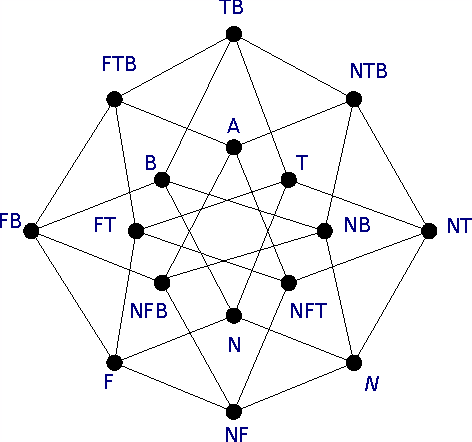
\includegraphics[width=0.6\textwidth]{img/Generalized_Truth_Values_and_Multilattices.pdf}
        \caption{ Treillis issue de la combinaison des valeurs de vérité (T,F,B,N). L'agrégation de toutes les valeurs de vérité est représenté par la lettre A ("all"). Cette figure représente les valeurs de vérité selon trois axes, (i) la vérité "t", (ii) la fausseté "f$^{-1}: t -f $", (iii), l'information notée "i". Ce treillis est appelé par \textit{Shramko et al.} "Trilattice Sixteen$_{3}$".  }
        \label{fig:sixteen_truth_values}
    \end{shadedfigure}

    \paragraph{Logique modale}
    La Logique modale est une extension de la logique propositionnelle. Elle permet de raisonner sur l'incertain et les situations évolutives. C’est la raison pour laquelle la sémantique est plus expressive. Elle permet de moduler la notion de véracité avec des notions comme "obligatoire" $\square$ et "concevable" $\diamond$. Ainsi on peut émettre des propositions plus nuancées pour rechercher si elles sont vraies dans certains cas de figure. La véracité d'une proposition va être recherché dans des "mondes possibles". Typiquement lorsque l'on lance une pièce de monnaie. (i) La pièce tombe obligatoirement du côté PILE ou FACE, (ii) obtenir le côté PILE est aussi probable que le côté FACE, et (iii) il est impossible l'obtenir PILE et FACE en même temps. On comprend que les côté PILE et FACE sont deux mondes accessibles mais ils ne peuvent pas être tous les deux vrais dans un même monde (i.e pour une même pièce à un même instant donné).
    
    Cette idée peut être généralisée de la façon suivante:\nolisttopbreak
    \begin{enumerate}[label=\roman*)]
        \item $\square A$ est vraie dans un monde possible ω, si A est vraie dans tous les mondes possibles accessibles à partir de ω.
        \item $\diamond A$ est vraie dans un monde possible ω, si A est vraie dans au moins un monde possible accessible à partir de ω.
        \item $\square A \land \square B$ est obligatoirement faux dans un monde ω, si $\square A \to \lnot \square B \lor \square B \to \lnot\square A$
    \end{enumerate}

    La logique modale permet d'exprimer quatre notions ( et plus en les combinant ):\nolisttopbreak
    \begin{enumerate}[label={}]
        \item $\square p$: p est nécessaire / obligatoire
        \item $\lnot\square p$: p est contingent / incertain
        \item $\diamond p$: p est possible / concevable
        \item $\lnot \diamond p$: p est impossible
    \end{enumerate}

    Il existe une multitude de logiques modales, par exemple les logiques temporels, épistémiques, déontiques ou encore les logiques alétiques. Chacune d'elle apporte une nuance aux différentes modalités ($\square \diamond$).
    
    \begin{tabular}{ll}
        temporelle:    & il va faire un beau temps \\
        épistémique:   & l'agent sait qu'il fait un beau temps,  l'agent croit qu'il fait un beau temps \\
        déontique:     & il doit faire un beau temps \\
        alétique:      & il est possible qu'il fasse un beau temps \\
    \end{tabular}

    Bien que je n'ai pas fait ce choix dans la suite  de mes travaux, ce type de formalisme pourrait s’appliquer à des problèmes en biologie de prédiction de fonctions et d’interprétation de phénotypes, notamment à travers les notions : "requis", "interdit", "incertain" et "peut être".  De plus également les notions de prédiction et d'expectation ont un sens proche de ce qui est exprimé en logique épistémique ("on croît" / "on sait"). De même, les trous dans les connaissances, comme les réactions orphelines de gènes,s’apparentent à  une formulation proche de la logique déontique.
    
    
    
    \subsubsection{Logique de description}
    
    La logique de description est un domaine de la logique permettant d'établir des faits à partir d’une représentation structurée de la connaissance. C'est une composante de l'intelligence artificielle qui dernière nécessite de représenter les connaissances afin de pouvoir calculer/déduire de nouveaux savoirs. Dans les grandes lignes, ce domaine s'attache à caractériser les catégories d'objets puis à les mettre en relation. La représentation des connaissances puis le raisonnement appliqué sur ces connaissances permettent la construction d'applications intelligentes ayant la capacité de trouver des conséquences implicites à partir de connaissances explicites.
    
    Une telle structuration des connaissances forme un réseau dont les individus sont des concepts (les nœuds) qui exposent différents types de lien. Le mot terminologie est employé dans ce domaine pour décrire les intentions données lors de la construction d'une structure hiérarchique. Et la sémantique utilise la terminologie pour étudier ce qui est signifié.
    
    \paragraph{Représentation des connaissances}
    La structuration hiérarchique des connaissances permet une représentation compacte et compréhensible de l'information. Mais surtout elle permet d'appliquer un raisonnement logique sur ces connaissances.
    
    Par exemple, une structuration hiérarchique de concepts reliés les uns aux autres par des relations symbolisant le "ET" et le "OU" sont efficacement disposés lorsque l'arbre est une disjonction de clauses.
    En effet dans de tels cas on peut rechercher indépendamment la véracité de l'un ou de l'autre littéral. Il suffit d'établir qu'un des deux littérals soit vrai pour déduire que la clause est vrai à son tour. Une telle structuration est une forme normale disjonctive.
    
    Évidement la logique de description n'est pas limitée aux relations ET/OU. Des sémantiques, comme celles proposées dans \acrfull{GO}, dispose de relation pour exprimer la composition et l'identité. Pour cela  \acrfull{GO} propose un vocabulaire contrôlé appelé l'ontologie, qui permet d’annoter la fonction biologique des gènes. Par ailleurs, on ne peut pas parler de la représentation des connaissances sans citer le web sémantique (standardisé par le W3C \footnote{W3C, est un organisme de standardisation à but non lucratif, fondé en octobre 1994 chargé de promouvoir la compatibilité des technologies du World Wide Web.}). Le web sémantique incarne un effort important de la communauté à fournir les outils et les méthodes pour analyser l'information dans son sens le plus générale. Une fois l'information structurée, des méthodes de raisonnement sur ces données peuvent être appliquées.
    
    \paragraph{Programmation logique}
    La logique est notamment utilisée pour simuler un raisonnement. Pour cela on définit un ensemble de règles logiques permettant de traiter un ensemble de faits élémentaires. Ainsi, les faits respectant les contraintes d'une règle se voient attribuer les conséquences logiques décrites par la règle. Cette approche s'apparente à la programmation d'une logique. De nombreux outils et méthodes permettent de mettre en œuvre un raisonnement logique basé sur des règles. Une règle est généralement composée de deux parties. La première est un ensemble de clauses et la seconde correspond à la conséquence logique.
    Une clause est une suite de littéraux reliés par des opérateurs de conjonction et disjonction. Un littéral est un atome avec ou non sa négation. Un atome est une proposition élémentaire vrai ou fausse. La conséquence logique est activé si le calcul des propositions pour un fait est établi comme vrai. Le langage \texttt{PROLOG} \cite{colmerauer1990introduction,clocksin2003programming} permet de résoudre des problèmes impliquant des objets\footnote{La notion d'objet au sens \texttt{PROLOG} est une entité représentable par un terme (oiseau par exemple). }
    
    \paragraph{Chaînage avant et arrière} %backward/forward
    Un raisonnement peut être décrit par une suite de règles. Une telle règle comporte deux parties. La première partie sélectionne les informations correspondant à une contrainte. Par exemple, tous les faits respectant la contrainte "x est une transaminase" seront sélectionnés. La deuxième partie correspond aux conséquences logiques. Pour faire suite à l'exemple précédent : "alors x est une protéine" . Ces deux parties forment une règle d'inférence. Les conséquences logiques d'une règle peuvent activer de nouvelles règles. Par la méthode du chaînage avant, les faits (des prémisses) sont utilisés pour remonter aux conclusions. Ce processus de déduction se poursuit tant qu'il existe des faits respectant les contraintes des règles.
    
    Prenons les trois règles suivantes:\nolisttopbreak    
    \begin{enumerate}
        \item Si x est une transaminase alors x est une protéine
        \item Si x est un ARN alors x est composé d'acides ribonucléiques
        \item Si x est une protéine alors x est composé d'acides aminés
    \end{enumerate}

    Lorsque le moteur d'inférence traite le fait "aspartate aminotransférase" la règle \ding{172} est activée et  conclue que le fait est une protéine. Cette conséquence va permettre d'activer à son tour la règle \ding{174} et conclure sur sa composition (en acides aminés). Aucun fait restant ne peut activer une règle, le raisonnement prend fin.
    
    Il est également possible, par la méthode du chaînage arrière, de partir des conclusions pour revenir aux prémisses. Ces méthodes de chaînage sont mises en œuvre à travers des moteurs d'inférence.
    
    \paragraph{Système expert}
    La mise bout à bout des connaissances, des règles d'inférence et des faits observés permet de capturer une partie du système cognitif d'un expert d'un domaine particulier ( un bio-curateur par exemple). Cet ensemble forme un système expert (voir \cref{fig:systeme_expert}). Ce procédé est utilisé notamment pour la mise en œuvre de l'intelligence artificielle. Le système dispose d'une base de faits, une base de règles et d'un moteur de règle. Les déductions réalisées à partir des faits observés permettent dans certains cas d'acquérir de nouvelles connaissances; cela se traduit par la formulation de nouvelles règles. Cet apprentissage automatique permet de dépasser le cadre théorique imposé par les règles de départ et d'imiter le comportement d'un expert faisant preuve d'adaptabilité face aux problèmes.
    
    \begin{shadedfigure}[H]
        \centering
        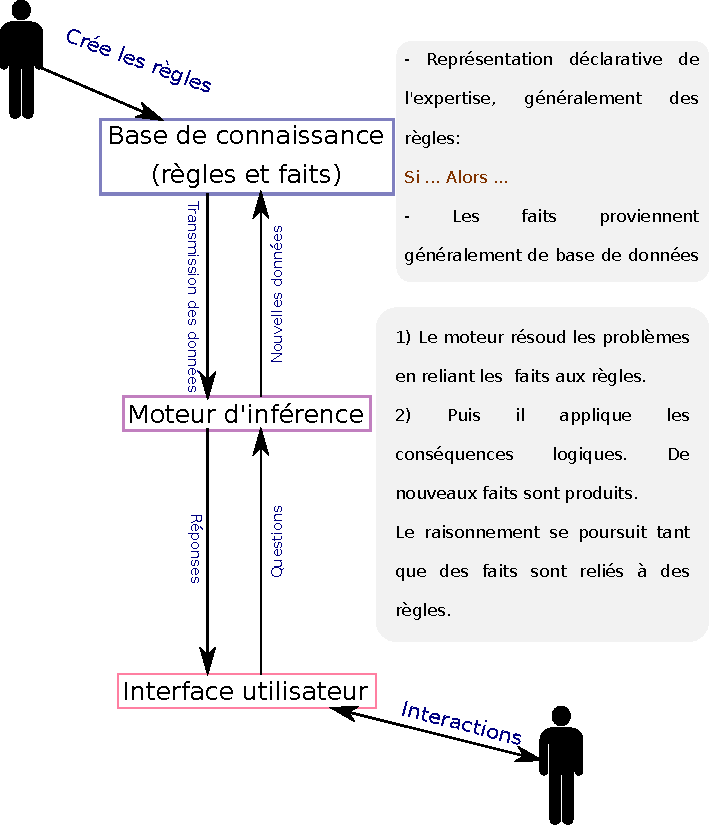
\includegraphics[width=\textwidth]{img/systeme_expert.pdf}
        \caption{Présentation des principaux composants d'un système expert.}
        \label{fig:systeme_expert}
    \end{shadedfigure}
    
    \section{Méthodes existantes}
    
    Dans le domaine de la biologie, et plus précisément dans le contexte de l’annotation fonctionnelle des gènes ou protéines, il existe plusieurs ressources qui utilisent des systèmes à base de règles. Ils vont être présentés dans cette section : \texttt{UniRule}/\texttt{HAMAP}, "\texttt{Genome Properties}" et "\texttt{IMG terms}". D’autres méthodes utilisent des modèles métaboliques.
    
    \subsection{UniRule}
    Afin de mimer l'expertise humaine sur l'annotation de plusieurs millions de protéines, le consortium \texttt{UniProt} a mis en place un outil à base de règles appelé \texttt{UniRule} \cite{unirule2015,bridge2010unirule}. Il s'agit d'une base de règles unifiant les règles provenant d'\texttt{\gsl{HAMAP}}, \texttt{\gsl{PIR}} et \texttt{RuleBase} . \texttt{UniRule} est utilisée conjointement avec le système \acrfull{SAAS} \cite{kretschmann2001automatic,uniprot2015}  qui génère des règles d’une manière automatique en utilisant les annotations expertisée par Swiss-Prot comme contrôle (voir Figure~\cref{fig:unirule}).
    
    \begin{shadedfigure}[H]
        \centering
        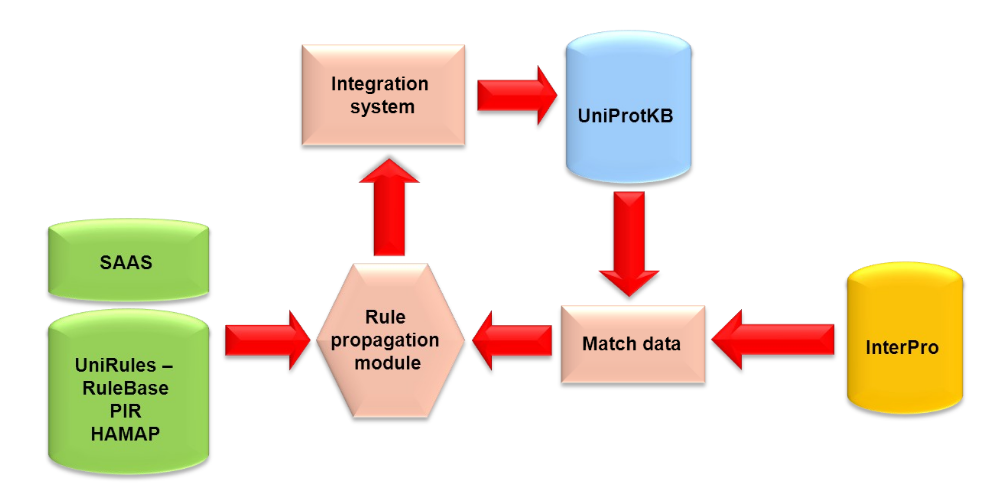
\includegraphics[width=\textwidth]{img/unirule.png}
        \caption{ Chaînage d'application pour l'annotation automatique des protéines la base de données UniProt. Figure extraite de \citetitle{bridge2010unirule}. }
        \label{fig:unirule}
    \end{shadedfigure}

    Les règles \acrshort{PIR} sont de deux types. Celles qui regroupe annotent des sites protéiques comme des sites catalytiques d’enzymes (\acrfull{PIRSR} \cite{vasudevan2011structure}) et celles qui réalisent des annotations textuelles comme la description des fonctions moléculaires (\acrfull{PIRNR}). Les règles \acrfull{PIRSR} sont validées humainement. Ces règles d'annotation ont une précision atomique. C'est-à-dire que la composition de la séquence protéique est utilisable pour déclencher une règle.
    
    \gls{HAMAP} est un système automatique de classification et d'annotation des séquences protéiques. Il est maintenu par le groupe \texttt{Swiss-Prot} . \gls{HAMAP} se base sur des profiles de séquences protéiques et des règles d'annotation fonctionnelle validés par des experts du domaine. Le système classifie automatiquement les séquences dans une des familles à partir des profiles en utilisant l’homologie de séquence. La syntaxe des règles  \gls{HAMAP} permet une grande expressivité et utilise le vocabulaire contrôlé d'\texttt{UniProt} et les termes \gls{GO} (présenté dans \url{http://hamap.expasy.org/unirule/unirule.html}). Tout comme les règles provenant de \gls{PIR}, \gls{HAMAP} peut effectuer des choix d'annotations selon la composition en acides aminé de la séquence protéique ce qui permet, par exemple de déclarer des résidus clefs, pour la fonction à transférer. Ces systèmes à base de règles sont un des moyens de stopper la propagation des erreurs d'annotations dans les ressources publiques \cite{schnoes2009annotation,devos2001intrinsic,bell2013can,gilks2002modeling}. Les annotations amenées par \gls{HAMAP} sont très variées et concernent de nombreux champs tels que: le nom du gène, les fonctions biologiques (transporteurs, les activités catalytiques, etc.), la localisation intracellulaire, les interactions protéines-protéines (voir \cref{fig:regle_unirule}).
    
    \begin{shadedfigure}[H]
        \centering
        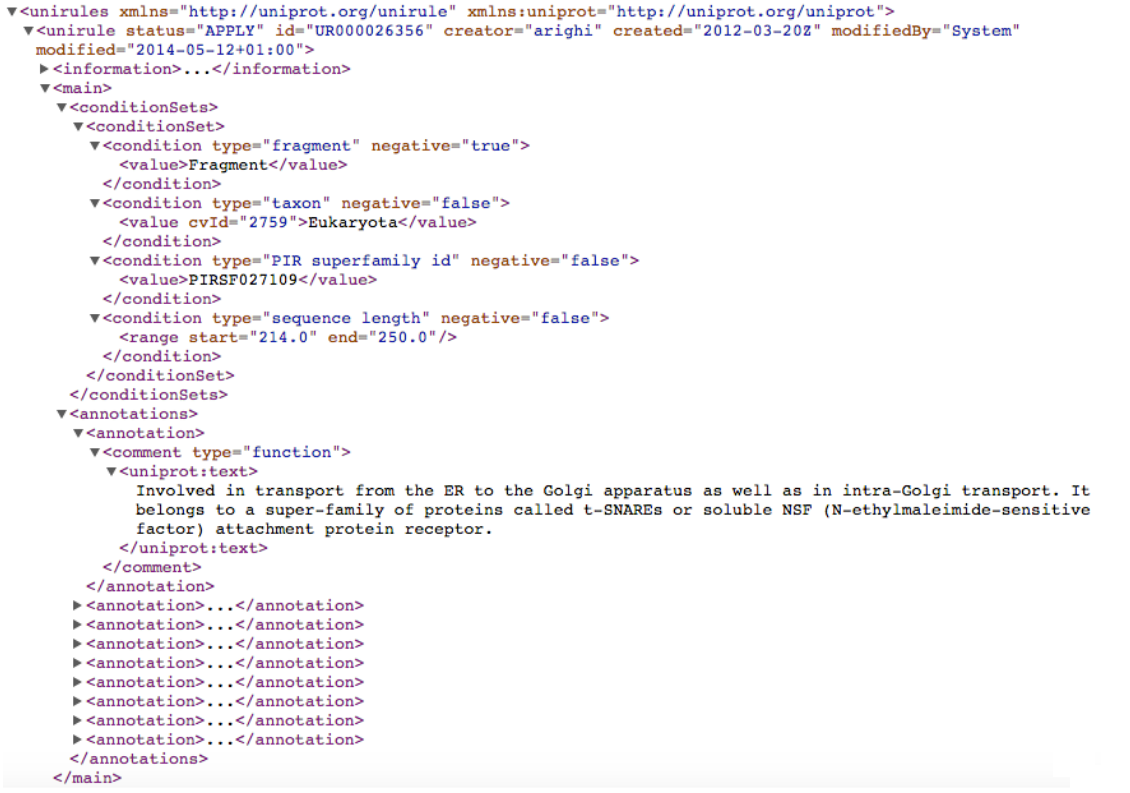
\includegraphics[width=\textwidth]{img/regle_unirule.png}
        \caption{Extrait d'une règle provenant d'\texttt{UniRule}. }
        \label{fig:regle_unirule}
    \end{shadedfigure}
    
    
    
    \subsection{Genome properties}
    
    Cette ressource part du constat qu'il est plus aisé d'annoter les protéines lorsqu'elles sont placées dans un contexte métabolique. Les informations de présence/absence d'une voie métabolique ou encore les réactions la composant, fournissent de précieuses informations pour l'annotation des protéines. Ainsi \texttt{Genome Properties} \cite{selengut2007tigrfams,haft2005genome,haft2013tigrfams} organise les processus biologiques clefs d'organismes procaryotes dans une structuration hiérarchique (voir Figure~\cref{fig:gp_lysine}). À travers un vocabulaire contrôlé les propriétés reflètent des phénotypes, des données taxonomiques ou encore des voies métaboliques.  Ces propriétés sont prédites à partir d’évidences qui sont, pour les voies métaboliques, des résultats d’alignement des protéines de l’organisme avec des profils de \gls{HMM}. Ces évidences permettent ainsi de déterminer si les différents composants (e.g. complexes protéiques et réactions) d’une voie métabolique sont présents. 
    
    \begin{shadedfigure}[H]
        \centering
        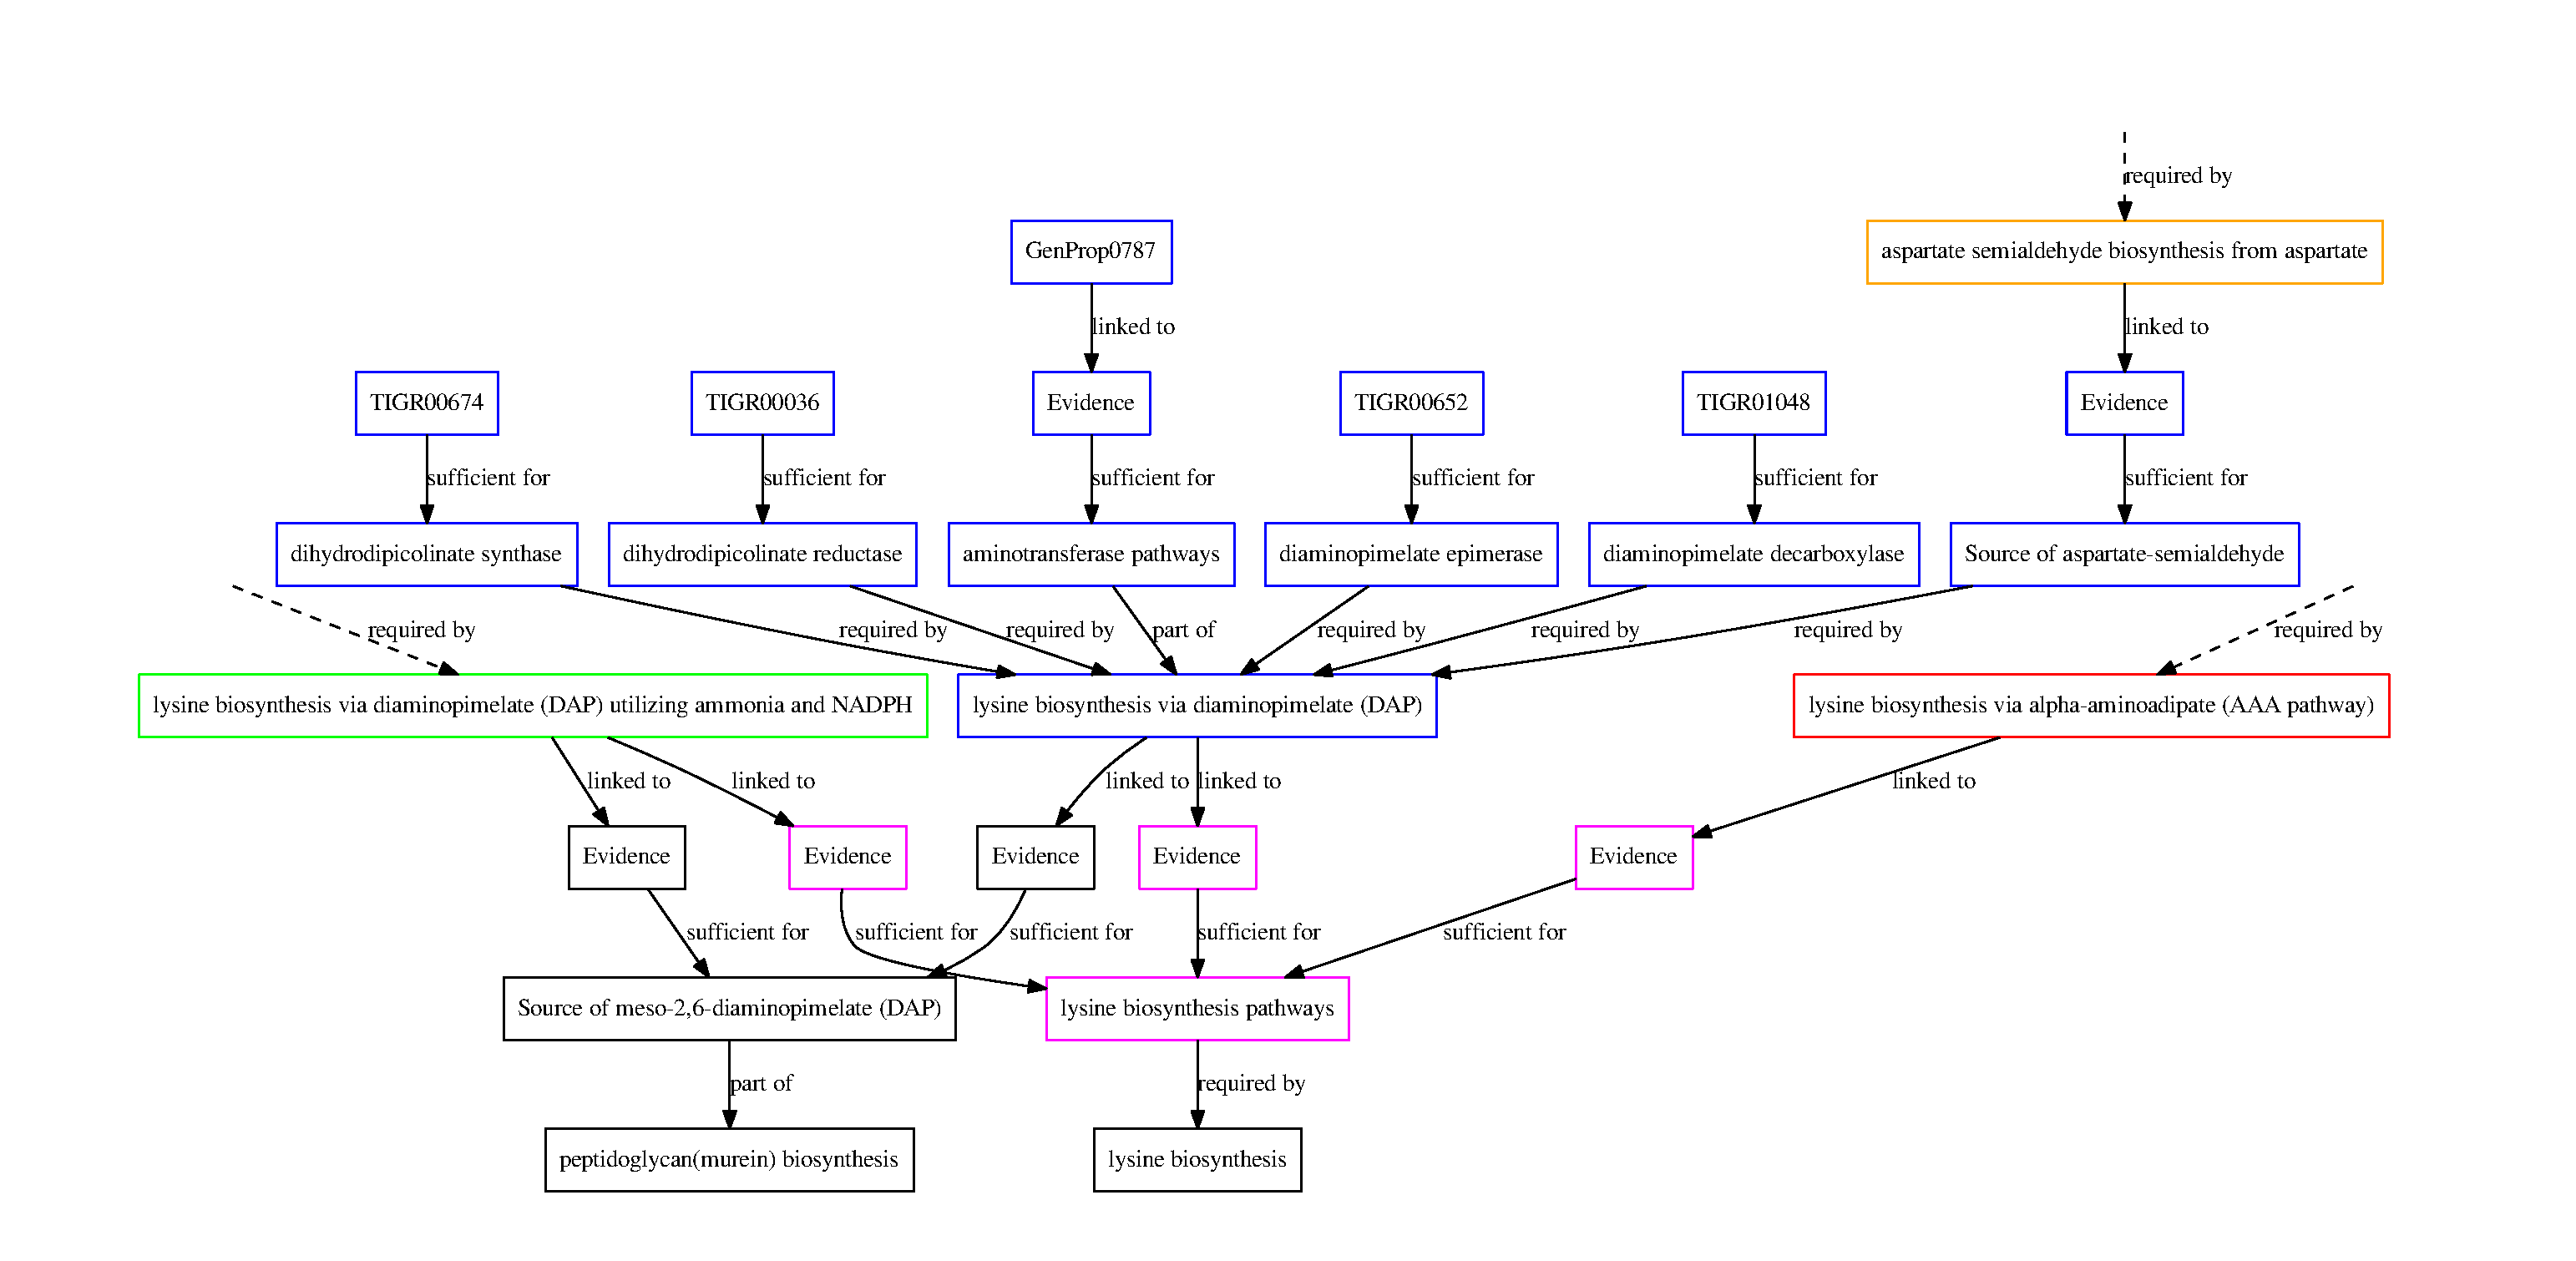
\includegraphics[width=\textwidth]{img/lysine_biosynthesis.pdf}
        \caption{ Représentation graphique de l'organisation des données au sein de \texttt{Genome Properties}. Au centre, la voie métabolique de la biosynthèse de la lysine via l'utilisation du diaminopimelate. }
        \label{fig:gp_lysine}
    \end{shadedfigure}

    Les données de  la ressource \texttt{Genome Properties} étaient extraites de la ressource de données microbiennes appelée \gls{CMR} \cite{peterson2001comprehensive,davidsen2009comprehensive}. La ressource \gls{CMR} n’est malheureusement plus maintenue. Pour les évidences, deux ressources de profils \gls{HMM} sont utilisées \texttt{TIGRFAM} \cite{haft2003tigrfams}\label{key} et \texttt{Pfam} \cite{bateman2000pfam,bateman2002pfam,bateman2004pfam,finn2008pfam,finn2009pfam,punta2011pfam,finn2013pfam,finn2016pfam}. Ainsi, la hiérarchie de \texttt{Genome Properties} est un ensemble de triplets évidence - composant - propriété (voir Figure~\cref{fig:gp_modele}). À partir de cette structure hiérarchique, des règles composées de conjonctions et disjonctions d’évidences vont être évaluées pour assigner une conclusion à chaque propriété :
    \begin{itemize}
        \item "Yes", tous les composants sont prédits, la propriété est présente
        « Some evidence », certains composants ne sont pas prédits mais la propriété peut être présente dans l’organisme
        \item "Not supported", suivant un seuil défini de complétion pour chaque propriété, le nombre de composants prédits n’est pas suffisant pour déterminer la présence de la propriété
        \item "None found", aucun composant prédit donc la propriété n’est pas présente dans l’organisme
        \item "No", un bio-curateur conclue que la propriété n’existe pas dans l’organisme
        "Cryptic", un bio-curateur conclue que la propriété n’est plus fonctionnelle dans l’organisme malgré la présence de composants
    \end{itemize}
    
    Dans cette évaluation, certains composants sont étiquetés comme « non essentiels » et ne sont donc pas pris en compte pour le calcul de la complétion des propriétés. Il peut s’agir de composants accessoires ou de composants difficiles à prédire.
    
    \begin{shadedfigure}
        \tikzset{
            treenode/.style = { shape=rectangle     , rounded corners,
                                draw, align=center  ,
                                top color=white     , bottom color=blue!20},
            root/.style     = {treenode, font=\Large, bottom color=red!30},
            other/.style    = {treenode, font=\ttfamily\normalsize},
        }
        \begin{tikzpicture}
        [
            grow                    = down,
            sibling distance        = 16em,
            level distance          = 5em,
            edge from parent/.style = {draw,color=black, -latex, <-},
            every node/.style       = {font=\footnotesize,color=black},
            execute at end picture=%
            {
                \begin{pgfonlayer}{background}
                \path[fill=white]
                (current bounding box.south west) rectangle
                (current bounding box.north east);
                \end{pgfonlayer}
            }
        ]
        \node[root]{Property}
            child { node [other] {Component}
                child { node [other] {Evidence}
                    child{ node [root] {Property}
                        child{ node [other] {Component}
                            child { node [other] {Evidence}
                                edge from parent node [above right]  {sufficient for} }
                            node[above right=0.2em and 3em,color=blue,font=\tiny]{is dispensable*}
                            edge from parent node [above,sloped] {part of}}
                        child{ node [other] {Component}
                            child { node [other] {Evidence}
                                edge from parent node [above right]  {sufficient for} }
                            edge from parent node [above,sloped] {part of}}
                        edge from parent node [above right]  {is a} }
                    edge from parent node [above right]  {sufficient for} }
                edge from parent node [above,sloped] {part of} }
            child { node [other] {Component}
                child { node [other] {Evidence}
                    edge from parent node [above right]  {sufficient for} }
            edge from parent node [above,sloped] {part of} };
            
            
        \end{tikzpicture}
        \caption{Modèle de la structure hiérarchique utilisée pour représenter les concepts au sein de \texttt{Genome Properties}. Des méta-informations peuvent être attachées aux nœuds permettant notamment d'indiquer s'ils sont facultatifs ("dispensable").  }
        \label{fig:gp_modele}
    \end{shadedfigure}
    
    \subsection{IMG terms}
    
    \texttt{IMG terms} \cite{chen2013improving} est certainement la méthodologie la plus proche de celle présentée dans cette thèse. Elle cherche à être robuste aux données biologiques erronées. Comme nous l’avons vu dans la section \ref{subsec:lacunes} \nameref{subsec:lacunes} les données et prédictions biologiques peuvent être partielles et contradictoires. Comme dans \texttt{Genome Properties}, les règles d’inférence de voies métaboliques sont représentées sous la forme de conjonctions et de disjonctions de réactions :
    
    \begin{equation}
    IMG_{reaction1} \; AND \; (IMG_{reaction2} \; OR \; IMG_{reaction3} ) \to IMG_{pathway 1}
    \end{equation}
    
    Les réactions ("\texttt{IMG reaction}") et voies métaboliques ("\texttt{IMG pathway}") sont décrites à l’aide d’un vocabulaire contrôlé les termes \texttt{IMG} ("\texttt{IMG terms}"). Chaque réaction \texttt{IMG} est associée à un prédicteur spécifique permettant de détecter à partir du génome d’un organisme des séquences de protéines catalysant la réaction. Si aucune prédiction n’est trouvée pour une réaction, une méthode, basée sur l’analyse des résultats de similarité de séquence avec des protéines connues pour catalyser la réaction, est appliquée pour déterminer si une protéine candidate pourrait catalyser la réaction. Pour chaque voie métabolique, IMG associe une des conclusions suivantes :
    \begin{itemize}
        \item "Asserted", la voie est présente car toutes ses réactions sont prédites
        \item "Not-asserted" la voie n’est pas présente car certains composants ne sont pas prédits et aucune protéine candidate n’a été détectée
        \item "Unknown", certaines réactions ne sont pas prédites mais des protéines candidates sont détectées.
    \end{itemize}

    Pour la prédiction de phénotypes, un deuxième niveau de règles d’inférence est représenté sous la forme de conjonctions et de disjonctions de voies métaboliques. Pour calculer ces propositions, \texttt{IMG} emploie une logique tri-valuée avec les trois états de conclusion des voies métaboliques : vrai ("Asserted"), faux ("Not-asserted"), ou inconnu ("Unknown" ).
    
    Bien que non déclarées comme telles dans leur article \citetitle{chen2013improving}, les auteurs utilisent les mêmes tables de vérité que celles décrites par \textit{Kleen} et \textit{Priest} (cf la partie \ref{par:logic_multivalued}  \nameref{par:logic_multivalued}). 
    
    \subsection{Méthodes utilisant des modèles métaboliques}
    
    En biologie des systèmes\footnote{Domaine d'étude des relations et des interactions entre différentes parties du système biologique.} une approche souvent utilisée pour l'étude des réseaux biochimiques d'un organisme est le \gls{FBA}\cite{orth2010flux}. L'objectif est de reconstruire un modèle métabolique \textit{in silico} permettant la production de la biomasse\footnote{Ensemble de métabolite considéré comme nécessaire aux développement de l'organisme} nécessaire au développement et à la reproduction de l'organisme d'intérêt. La modélisation du réactome permet d'émettre des hypothèses et de faire des prédictions sur la croissance d'un organisme dans un milieu nutritionnel défini. Les capacités d'un organisme sont alors étudiées par simulation ,dans une infinité de conditions.
    
    Ce type de méthode nécessite tout d’abord de décrire mathématiquement les flux de métabolites. Pour chaque réaction, les coefficients stœchiométriques des acteurs de la réaction (substrats, produits, co-facteurs, etc., cf. \cref{subsec:acteurs} \nameref{subsec:acteurs}) sont renseignés dans une matrice réactions/métabolites. Cette matrice est employée pour contraindre la production de métabolites de telle sorte qu’elle soit égale à la quantité de métabolite consommée et produite à l’état stationnaire\footnote{L'état stationnaire représente un moment où les métabolites sont consommés et produits lors d'une réaction.}. La stœchiométrie oriente le flux des métabolites à travers le réseau de réactions. Ce flux est contraint de respecter l’équilibre des réactions. Toutefois cette contrainte ne tient pas compte de la cinétique des réactions \cite{covert2001metabolic,edwards2002metabolic}\footnote{Il existe d'autre méthode utilisant à la fois les modèles métaboliques et la cinétique des réactions tels que l'approche \gls{MCA}. De tels approches sont complexes, car elles nécessitent d'établir la cinétique de toutes les réactions ayant lieu \textit{in vivo} et également la concentration des métabolites.}. L’inégalité des proportions de métabolites utilisés en entrée et en sortie impose des limites au système. En réponse à cette contrainte, une proportion minimum et maximum de flux autorisés est définie pour chaque réaction. D’autres contraintes peuvent aussi être ajoutées.
    
    Une fois le modèle mathématique décrit, il est possible de rechercher les meilleures conditions de croissance pour un organisme. Prédire le développement optimal d’un organisme revient à calculer le flux maximum conduisant à la production de biomasse. En d’autres termes, les flux seront optimisés pour atteindre les réactions permettant la production de la biomasse. Mathématiquement cela revient à définir, de façon quantitative, dans quelle proportion chaque réaction doit contribuer pour l’expression du phénotype. Par la suite, la production de la biomasse par modélisation peut être comparée aux résultats expérimentaux, permettant alors de valider ou non le modèle métabolique.
    
    
    Dans le cadre du \gls{FBA} la résolution de tels modèles passe souvent par l’utilisation de la programmation linéaire. En effet, cette approche permet la résolution de problèmes où l’on cherche à optimiser un objectif (nommé "fonction objectif"). Dans le domaine de la bio-informatique, l’utilisation de la méthode se justifie par le postulat suivant : l’évolution a conduit à des "organismes optimaux". Ainsi, selon les métabolites contenus dans le terme "biomasse", les flux optimaux varieront.
    
    Toutefois, pour produire de la biomasse, cette méthode requiert un modèle métabolique complet et de qualité. Autrement dit, des « fuites » de métabolites vont gêner, voire empêcher, l’optimisation des objectifs. Ainsi, des méthodes permettant de combler les « trous » dans le réseau métabolique ont été développées, par exemple \texttt{GapFill}\cite{kumar2007optimization}, \texttt{FastGapFill}\cite{thiele2014fastgapfill}, \texttt{Mirage}\cite{vitkin2012mirage}, \texttt{Meneco}\cite{prigent2017meneco}. Ces méthodes cherchent à établir de nouvelles "passerelles réactionnelles" afin de diriger le flux vers les objectifs de production. \texttt{GapFill} remplis les "trous" et optimise la synthèse de la biomasse, à partir de l’identification d’un nombre minimal de réactions nécessaires pour atteindre les objectifs. \texttt{FastGapFill} étend les fonctionnalités de \texttt{GapFill} en ne se concentrant plus uniquement sur la production de la biomasse, mais également en ajoutant des flux entrants et sortants au réseau métabolique. \texttt{Mirage} relâche la notion de "minimalité" de réactions à ajouter pour satisfaire les objectifs en utilisant les profiles phylogénétiques des espèces pour déterminer si une réaction doit être ajoutée ou non. \texttt{Meneco} se base sur la topologie du réseau pour remplir les "trous" : il va restreindre les réactions à ajouter aux métabolites produits via un chemin de réactions connectées aux substrats de sorte que les métabolites entrant dans le réseau soient topologiquement connectés.
    
    Ces différentes méthodes permettent de créer de nouveaux chemins à travers le réseau de réactions. Ces nouvelles réactions sont généralement issues de ressources publiques généralistes (comme \texttt{MetaCyc}, \texttt{KEGG}, etc). Les raccordements ainsi réalisés permettent d’avoir un modèle cohérent vis à vis de la quantité de biomasse produite supposée nécessaire à l’organisme. Le sens d’une réaction (unidirectionnelle, réversible \ldots) peut être également changé dans l’objectif d’optimiser encore un peu plus les flux de métabolites.
    
    \subsection{Méthodes utilisant d'autres systèmes logiques }
    
    Il existe également des méthodes logiques utilisant une notion de probabilité pour l'inférence d'état comme en logique inductive \cite{michalski1983theory,muggleton1994inductive}. Généralement elle se base sur une fouille de données. Après analyse de ces données il est possible de décrire la probabilité qu'un événement se passe et donc d'inférer des lois générales sur la base des événements avec un fort degré de "croyance". Dans un tel système le degré de "croyance" est un moyen de définir quelque chose comme probablement vraie. Cette notion de croyance se différencie du "vrai" défini en logique classique car elle est une affirmation non probabiliste. Ainsi la programmation par logique inductive permet de générer des hypothèses au regard des faits observés. Cette approche est nommée dans la littérature scientifique de la manière suivante : "\gls{ILP}". Ce domaine d'étude est à l'intersection de deux domaines, (i) l'apprentissage ("machine learning") et (ii) la programmation logique. Dans le domaine de l'annotation fonctionnelle des gènes, des approches utilisant l'\gls{ILP} ont été proposées à la communauté scientifique \cite{clare2003predicting,king2004applying}.
    
    Une autre approche part du principe qu'il est compliqué, voir impossible, de tout catégoriser en termes soit vrai soit faux. En effet, il existe des cas flous. En lieu et place des termes binaires, l'utilisation d'ensembles au contour flou permet de raisonner avec des données approximatives, incertaines ou manquantes. Cette méthodologie de raisonnement est appelée "logique floue" \ref{fig:fuzzy}.
        
    \begin{shadedfigure}[H]
        \centering
        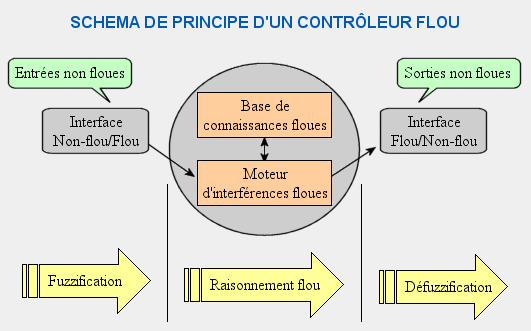
\includegraphics[width=\textwidth]{img/fuzzi-schema-controleur.png}
        \caption{Les données non floues sont transformées en données floues. Puis le moteur d'inférence va propager les conséquences logiques à travers des règles floues. Pour terminer les conséquences logiques sont retranscrites de  manière non floue par l'étape de "défuzzification",c'est-a-dire qu'un degré d'appartenance aux différents ensemble est attribuer. \hspace{\textwidth}\tiny{Source: \url{http://www.decformations.com/mathematiques/logique_floue.php}}}
        \label{fig:fuzzy}
    \end{shadedfigure}
    
    
    \subbibliography
\end{refsegment}
    
    \begin{refsegment}
\chapter{Investigations sur la logique paracohérente}

Comme évoqué précédemment, les données et prédictions en biologie peuvent être incomplètes et contradictoires. Ces trois années de recherche ont été consacrées à la conception d'une méthode et d'un logiciel qui a pour objectif d'aider les biologistes à évaluer les prédictions bio-informatiques pour l'annotation fonctionnelle des génomes au travers de processus biologiques. Un tel système expert doit donc être capable de gérer des annotations inconsistantes d'où le choix d'orienter mes travaux dans le cadre de la logique paracohérente.

\section{Contexte du projet}

Mon projet de recherche a débuté par l'identification des besoins et des outils à ma disposition. Les orientations technologiques de la plateforme \texttt{MicroScope} (i.e. plateforme d'annotation de génomes microbiens, développée dans le laboratoire où j'ai réalisé ces travaux) portaient sur trois axes.

Le premier correspondait à la modernisation du système de gestion et de déclaration des chaînages applicatifs ("wokflows"). Pour cela, la plateforme \texttt{MicroScope} s'oriente vers la mise en place d'un moteur à base de règles développé en interne au \texttt{GenoScope} (\texttt{\gls{BIRDS}}) . Le système utilise l'application \texttt{DROOLS}\cite{mcwhirter2001drools,browne2009jboss} pour raisonner et ordonner les processus à partir de règles métiers décrivant les ressources à utiliser et l'enchainement des programmes dans le processus d'annotation de génomes.

Le second axe consistait à la mise en place d'un système d'intégration des données métaboliques de la plateforme, dénommé \texttt{Galileo} \cite{galileo2014}. Cet outil a la faculté de réconcilier les informations provenant de multiples ressources externes et internes. Les informations contenues dans ces différentes ressources sont réunies dans une interface unique. Les informations sont extraites des ressources \texttt{ChEBI} \cite{hastings2013chebi}, \texttt{RHEA} \cite{alcantara2012rhea}, \texttt{KEGG} et \texttt{MetaCyc}. Ainsi, \texttt{Galileo} permet d'avoir accès à un large éventail d'information sur les connaissances métaboliques. 

Le troisième axe s'articulait autour d'un système à base de règles pour l'annotation des génomes. Il a pour objectif de guider le biologiste sur les annotations suspectées manquantes dans un organisme donné. Il est composé de deux modules. Le premier permet de récupérer les règles d'\texttt{UniRule} et de les rendre utilisables en dehors de "l'\gls{EBI}". Les règles d'annotation fonctionnelle établies à partir des domaines protéiques seraient ainsi partagées avec la communauté scientifique. Le deuxième module doit évaluer les fonctions prédites au regard des processus métaboliques et mettre en évidence des annotations confirmées, manquantes ou contradictoires. La cohérence des annotations d'un génome peut ainsi être évaluée vis-à-vis des attentes portées sur des processus que l'organisme est capable de réaliser. Le moteur de règles \texttt{DROOLS} a été choisi pour la mise en œuvre du raisonnement. Ce moteur est moderne et il est capable de communiquer avec des applications  \texttt{Java} ce  qui est un avantage car \texttt{Galileo} et \texttt{BIRDS} sont également écrits dans ce même langage.

C'est sur ce dernier axe que j'ai effectué mes recherches tout en échangeant avec les deux premiers afin de récupérer les prédictions bio-informatiques et les données métaboliques unifiées. Le contexte de mon projet de recherche a été présenté lors de la 10$^{ème}$ conférence internationale sur l'intégration de données en sciences de la vie (DILS 2014 \url{http://dils2014.inesc-id.pt/}).

\cleardoublepage
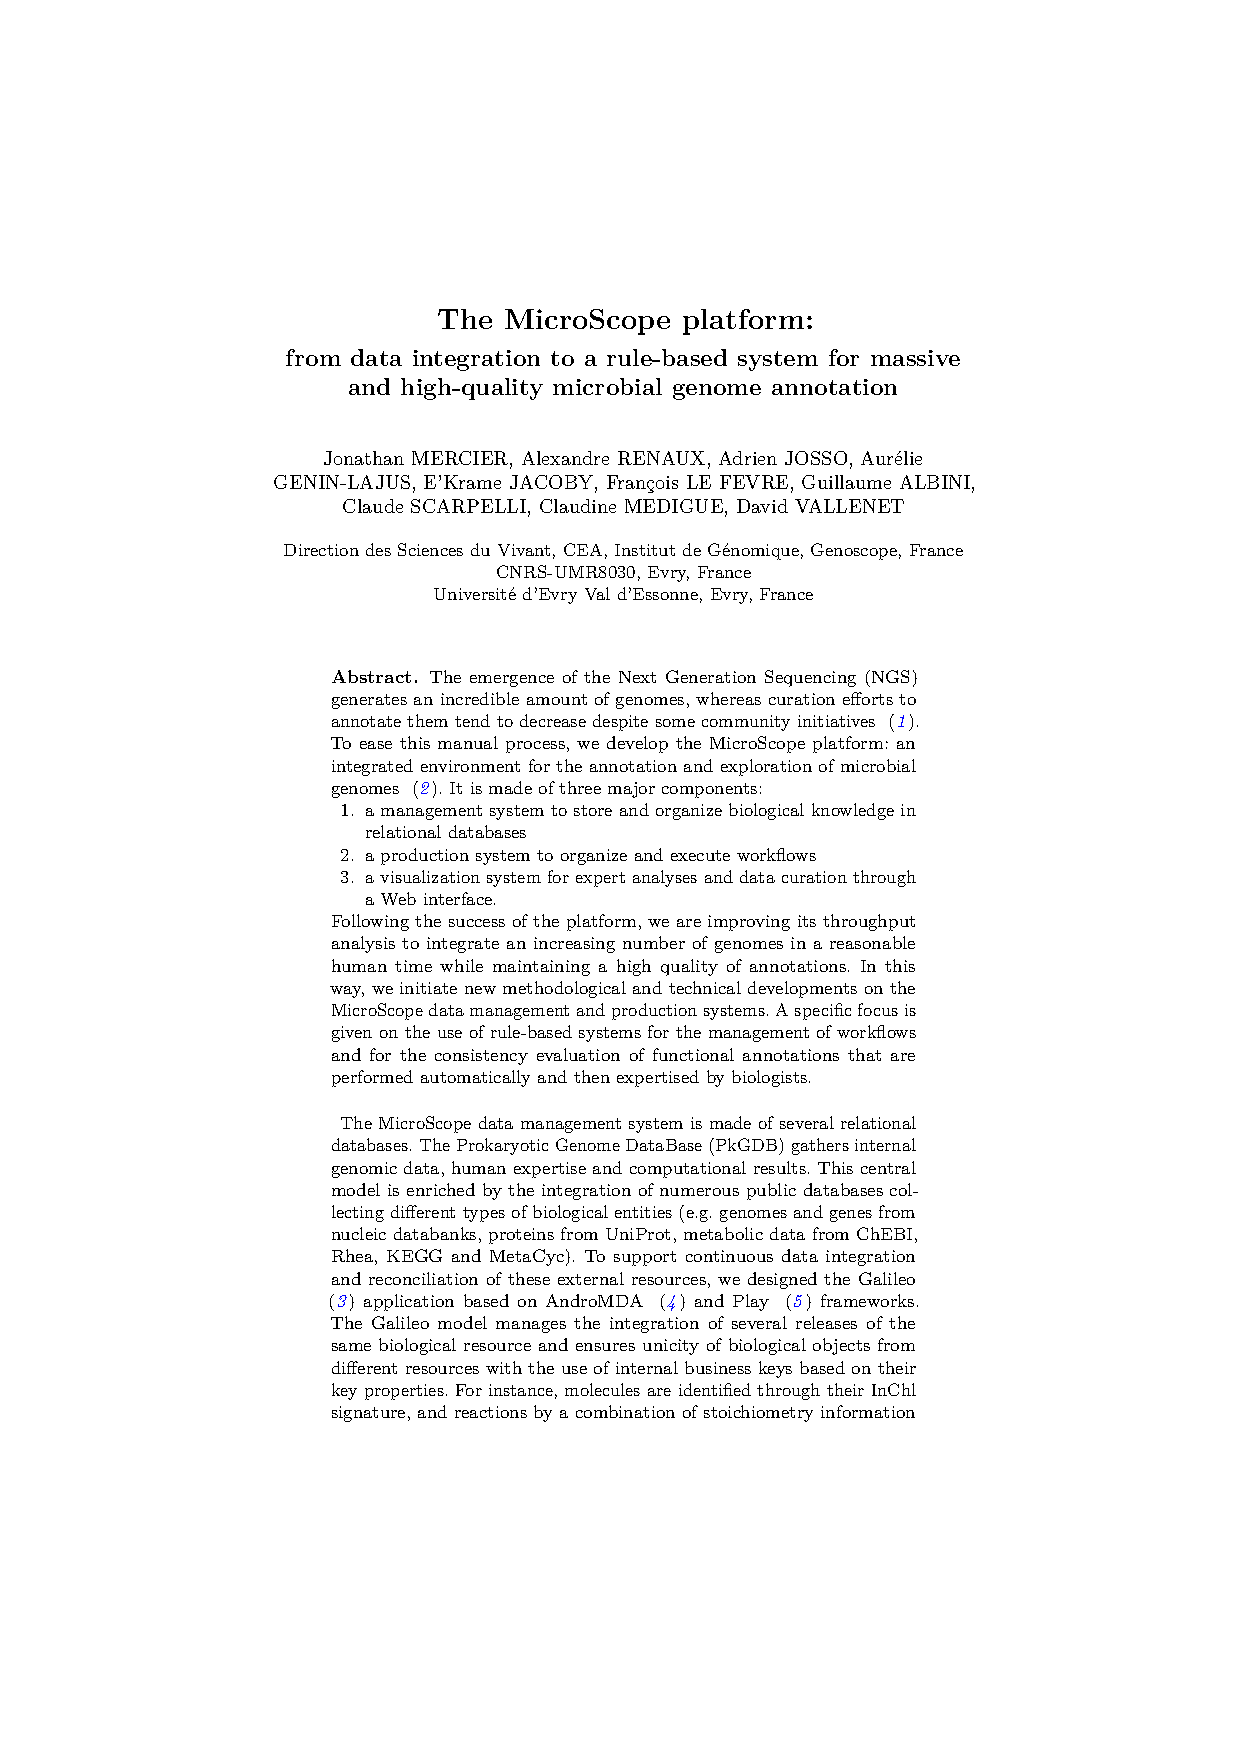
\includepdf[pages=-]{img/DILS_2014.pdf}

\section{HERBS}

L'équipe \texttt{HELIX}, dirigée par \textit{Alain VIARI}, avait commencé un projet en ce sens nommé \texttt{\gls{HERBS}}, en collaboration avec le \texttt{\gls{SIB}} dans le cadre du projet \gls{HAMAP} \cite{pedruzzi2015hamap}. L'objectif de \texttt{\gls{HERBS}} est d'alerter les biologistes sur les fonctions et les voies métaboliques manquantes, non attendues ou encore ambiguës. Pour cela, l'outil s'appuie sur le moteur d'inférence \texttt{\gls{JESS}}, sur une base de connaissance (contenant les règles et les faits, \cref{fig:systeme_expert}) et sur une interface graphique pour l'exploration des connaissances. 

Les connaissances dans \texttt{HERBS} sont structurées en trois composants :\nolisttopbreak
\begin{itemize}
    \item La base de connaissance contient des faits primaires sur l'organisme étudié (sa taxonomie  et des propriétés phénotypiques, exemple : l'organisme est photosynthétique), et des faits généraux décrivant des processus biologiques et leurs composants sous la forme d'un  graphe orienté acyclique avec des nœuds \texttt{ET} et \texttt{OU}.
    \item La base d'observations contient des prédictions d'unités fonctionnelles (i.e. composants de processus) dans l'organisme étudié.
    \item Des règles logiques permettant de prendre des décisions (e.g. SI X est requis par une bactérie et X n'est pas observé ALORS X est manquant dans l'annotation de la bactérie).
\end{itemize}

Le raisonnement dans \texttt{HERBS} se fait en propageant les observations au travers du graphe de connaissances par l'application des règles logiques. Chaque nœud est associé à trois attributs pouvant prendre les valeurs "oui" ou "non" au cours du raisonnement :\nolisttopbreak
\begin{itemize}
    \item "Présent", le composant est prédit ou non dans l'organisme
    \item "Requis", le composant est observé dans l'organisme (e.g. un phénotype de croissance)
    \item "Interdit", le composant n'est pas attendu dans l'organisme.
\end{itemize}

À la fin du raisonnement, des conclusions sur les processus et leurs composants sont données suivant cette table de correspondance :\nolisttopbreak
\begin{table}[H]
    \centering
    \label{tab:herbs_conclusion}
    \begin{tabular}{|l|l|l|>{\columncolor{LightCyan}}l|}
        \toprule
        \rowcolor{LightCyan}
        \textbf{Présent} & \textbf{Requis} & \textbf{Interdit} & \textbf{Conclusion} \\ 
        \midrule
        oui & oui & oui & ambigu \\ 
        \hline 
        oui & oui & non & normal \\ 
        \hline 
        oui & non & oui & inattendu \\ 
        \hline 
        oui & non & non & orphelin \\ 
        \hline 
        non & oui & oui & ambigu \\ 
        \hline 
        non & oui & oui & manquant \\ 
        \hline 
        non & non & oui & normal \\ 
        \hline 
        non & non & non & normal \\ 
        \bottomrule
    \end{tabular} 
\end{table}

\textit{Alain VIARI} m'a permis d'utiliser l'outil \texttt{PathRules}, une implémentation de \texttt{\gls{HERBS}} basé sur le moteur \texttt{\gls{CLIPS}} \cite{riley1991clips}. Pour tester ce logiciel, j'ai fourni à la base de faits les voies de biosynthèse de la lysine avec les variants \texttt{AAA} et \texttt{DAP} décrits par \texttt{UniPathway} et les prédictions d'activités enzymatiques provenant de l'analyse de 79 génomes. Pour ce faire, les données sont rangées dans trois dossiers présents à la racine du projet: (i) \texttt{data/processes} pour la description des voies métaboliques, (ii) \texttt{data/observers/uniprot} pour le catalogue des prédictions par espèce, (iii) \texttt{data/species} pour la description taxonomique des espèces. Les fichiers doivent porter l'extension \texttt{.data} et le nom du fichier est utilisé comme identifiant pour faire le lien entre les processus, les prédictions et les informations taxonomiques de l'espèce. Par exemple, j'ai utilisé l'identifiant \texttt{ACIAD} pour mettre en relation les informations d'\textit{Acinetobacter baylyi} ADP1.

\console{find data/ -name 'ACIAD.data'}{ data/observers/uniprot/ACIAD.data\par data/species/ACIAD.data }


La description des données dans ces fichiers suit la nomenclature \texttt{\gls{CLIPS}}, c'est-à-dire que les faits sont déclarés entre parenthèses. C'est la raison pour laquelle les observations sont formatées comme suit: 

( \texttt{source} (id \texttt{xxx}) (alias \texttt{yyy} sp:\texttt{zzz})  )

Extrait d'un fichier cataloguant les faits relatifs à un organisme:\nolisttopbreak

\console{head data/observers/uniprot/data/ACIAD.data}{
    (uniprot (id ASPARTATE-SEMIALDEHYDE-DEHYDROGENASE-RXN) (alias ACIAD0479 sp:ACIAD00423))\par
    (uniprot (id SUCCDIAMINOPIMDESUCC-RXN) (alias ACIAD0791 sp:ACIAD0070)\par
    (uniprot (id ASPARTATEKIN-RXN) (alias ACIAD1252 sp:ACIAD01133))\par
    (uniprot (id SUCCINYLDIAMINOPIMTRANS-RXN) (alias ACIAD2080 sp:ACIAD01886))\par
    (uniprot (id TETHYDPICSUCC-RXN) (alias ACIAD2599 sp:ACIAD02357))\par
    (uniprot (id DIAMINOPIMEPIM-RXN) (alias ACIAD2659 sp:ACIAD02412))\par
    (uniprot (id DIAMINOPIMDECARB-RXN) (alias ACIAD2660 sp:ACIAD02413))\par
    (uniprot (id DIHYDRODIPICSYN-RXN) (alias ACIAD3585 sp:ACIAD03222))\par
    (uniprot (id DIHYDROPICRED-RXN) (alias ACIAD3619 sp:ACIAD03252))\par
}


L'information taxonomique est également un fait. Il débute par le mot-clé "species" suivi de chaînes de caractères de plus en plus précises sur la taxonomie de l'organisme.

\console{cat data/species/ACIAD.data}{ (species lineage Bacteria Proteobacteria Gammaproteobacteria Pseudomonadales Moraxellaceae Acinetobacter Acinetobacter\_baylyi\_ADP1) }

Pour représenter la structure hiérarchique des voies métaboliques, les faits sont organisés pour exprimer la notion de composition et d'équivalence. La notion de composition est utilisée pour relier les ensembles de réactions (\gls{ULS} \texttt{d'UniPathway}) à leurs réactions. Quant à l'équivalence, elle permet de définir les chemins alternatifs (variants) pour réaliser une voie métabolique. La syntaxe \texttt{\gls{CLIPS}} utilise $x -> \ldots$ pour signifier "x tel que \ldots". La partie à droite de la flèche décrit les relations en notation polonaise\footnote{Également connue sous le nom "notation pré-fixée". Par exemple, le calcul "$5 \times (2 + 3)$", s'écrit "$\times 5 (+ 2 \qquad 3)$". }. Ci-après le fichier de description de la voie métabolique de la biosynthèse de la lysine par le variant \texttt{AAA} (Acide alpha-Amino Adipique) selon \texttt{UniPathway}.

\console{cat data/processes/lysine\_AAA\_biosynthesis.data}{
    ;;;; --------------------------------------------------------\par
    ;;; HERBS (Hamap Expert Rules Based System)\par
    ;;;\par
    ;;; @file: lysine\_AAA\_biosynthesis.data\par
    ;;; --------------------------------------------------------\par
    ;;;\par
    (process declare lysine\_AAA\_biosynthesis present in ALL)\par
    (process define lysine\_AAA\_biosynthesis -> and UPA00033)\par
    (process define UPA00033 -> or UPA00033-alt-0 UPA00033-alt-1)\par
    (process define UPA00033-alt-0 -> and ULS00012 ULS00013)\par
    (process define UPA00033-alt-1 -> and ULS00012 ULS00014)\par
    (process define ULS00012 -> and ULS00012-alt-0)\par
    (process define ULS00012-alt-0 -> and UER00028 UER00029 UER00030 UER00031 UER01027)\par
    (process define ULS00013 -> or ULS00013-alt-0 ULS00013-alt-1)\par
    (process define ULS00013-alt-0 -> and UER00032 UER00034)\par
    (process define ULS00013-alt-1 -> and UER00033 UER00034)\par
    (process define ULS00012 -> and ULS00012-alt-0)\par
    (process define ULS00012-alt-0 -> and UER00028 UER00029 UER00030 UER00031 UER01027)\par
    (process define ULS00014 -> or ULS00014-alt-0 ULS00014-alt-1)\par
    (process define ULS00014-alt-0 -> and UER00035 UER00037 UER00038 UER00039)\par
    (process define ULS00014-alt-1 -> and UER00036 UER00037 UER00038 UER00039)\par
}


Chaque processus est un fait, désigné par le mot-clé "process". Les voies métaboliques sont préfixées du mot-clé "declare" et "define" pour ses composants. Les faits constituant la voie métabolique sont hiérarchiquement organisés. Lorsqu'un fait est composé de plusieurs concepts, on utilise le symbole "and" et le symbole "or" lorsqu'un fait possède des équivalences. Les lignes débutant par un point virgule ne sont pas interprétées par \texttt{\gls{CLIPS}}. Elles permettent de commenter les règles et les faits.

À la fin du raisonnement, une évaluation de la complétion de l'annotation fonctionnelle des génomes est proposée sous la forme d'un tableau (\cref{fig:herbs_rapport}).

\begin{shadedfigure}[H]
    \centering
    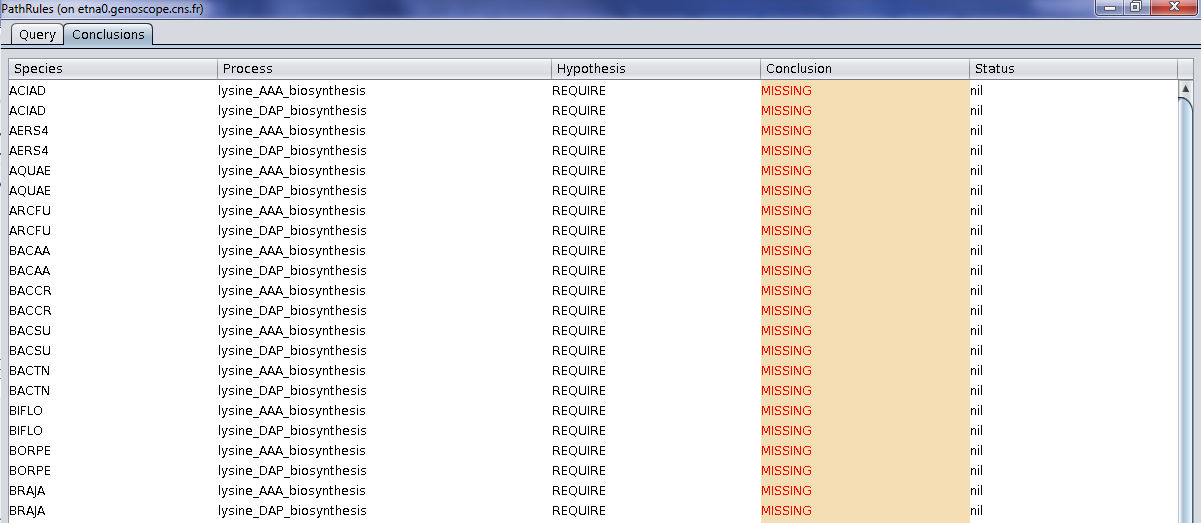
\includegraphics[width=\textwidth]{img/herbs_conclusion_report.png}
    \caption{Rapport sur la présence de la voie de biosynthèse de la lysine.}
    \label{fig:herbs_rapport}
\end{shadedfigure}

L'utilisateur a la possibilité d'explorer les résultats de \texttt{\gls{HERBS}} sur les voies métaboliques et leurs composants à travers un graphe orienté acyclique (\cref{fig:herbs_dag}).

\begin{landscape}
    \begin{shadedfigure}[H]
        \centering
        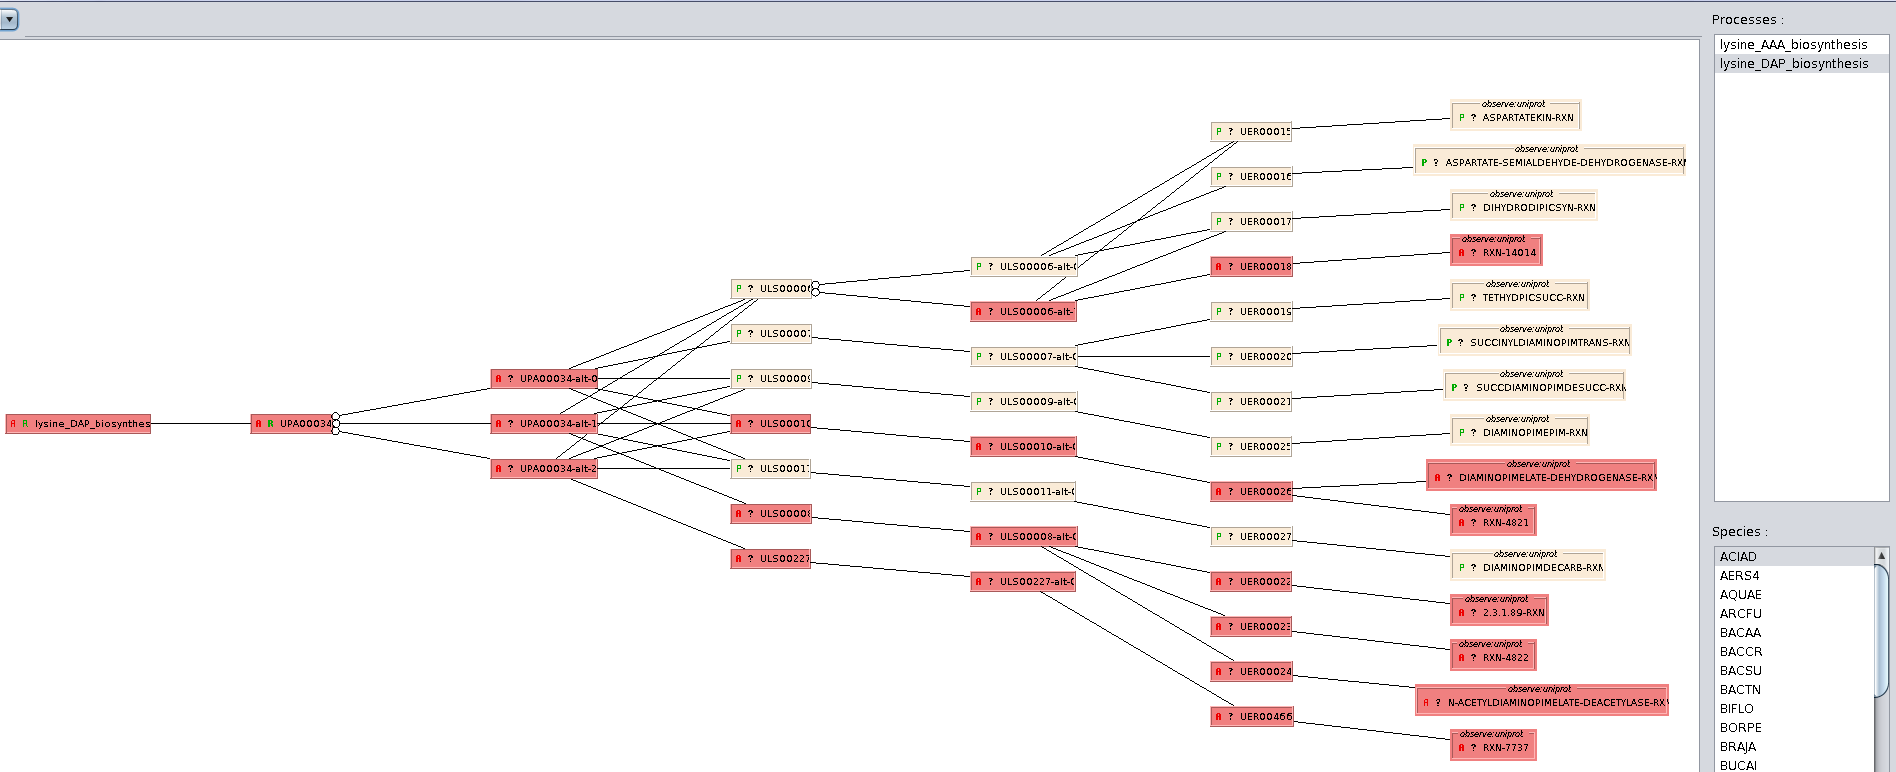
\includegraphics[width=\textwidth]{img/herbs_aciad_lysine_dap.png}
        \caption{Rapport sur la présence de la voie de biosynthèse de la lysine pour un organisme. La couleur jaune indique que la prédiction portée sur le concept est en accord avec les connaissances sur l'organisme. Dans le cas contraire, le concept est sur fond rouge. }
        \label{fig:herbs_dag}
    \end{shadedfigure}
\end{landscape}


Une des difficultés dans l'utilisation de \texttt{\gls{HERBS}} est tout d'abord de traduire toutes les connaissances sur les voies métaboliques et les prédictions en CLIPS. De plus, le système ne prend pas en charge la notion d'inconnu et la contradiction sur les prédictions. En effet, en biologie, l'absence de résultat suite à une expérience ou à une prédiction est souvent difficile à interpréter comme un résultat vrai négatif ou faux négatif. Ce point de vue peut paraître quelque peu philosophique. Il fait référence aux concepts de "monde ouvert" et "monde fermé". Une hypothèse en monde fermé va considérer toutes les questions sans réponse comme fausses. En monde ouvert, les hypothèses prennent la valeur vrai ou faux lorsqu'elles sont explicitement décrites comme telles. Pour les autres cas, une hypothèse est considérée incertaine tant qu'un fait ne la désigne pas comme vraie ou fausse. Dans l'exemple précédent de \texttt{\gls{HERBS}}, la plupart des voies métaboliques sont déclarées "Missing" sans pour autant suggérer quel variant est le plus plausible pour l'organisme d'intérêt. Ceci s'explique par le fait que, d'une part, un composant dans \texttt{\gls{HERBS}} est soit présent soit absent et, d'autre part, l'absence est propagée sur la voie métabolique même si d'autres réactions de la voie sont présentes. Ainsi, si une réaction est absente dans une voie métabolique alors cette voie sera considérée comme absente et aura la conclusion "Missing" ou "Normal" (\cref{tab:herbs_conclusion}). On pourrait s'attendre à ce qu'un système comme \texttt{\gls{HERBS}} soit capable de distinguer et suggérer des voies métaboliques en présence de données biologiques partielles ou contradictoires. 

\section{Première version de GROOLS}

\subsection{Logique et notion d'objet}

Au début de mes investigations, j'ai rencontré plusieurs difficultés. La première était d'utiliser les données structurées et complexes issues de la biologie à travers des règles de logique. Il faut savoir que la plupart des raisonneurs (comme \texttt{Prolog} et \texttt{CLIPS}) utilisent la programmation déclarative, ce qui consiste à décrire le problème\footnote{Par opposition a des langages comme Java, Python, D, Perl \ldots, ils utilisent la programmation impérative qui s'attache à décrire comment trouver la solution.}. La déclaration de problèmes impliquant des données structurées n'était pas initialement prévue dans ce paradigme\footnote{Des extensions du paradigme ont permis d'utiliser des structures de données complexes comme Prolog++.}. Par exemple, un bloc de réactions composé  des réactions A et B peut s'exprimer par la règle suivante (en Prolog):

\begin{lstlisting}[basicstyle=\small\normalfont\ttfamily,language=Prolog]
    reaction_block(Arg1, Arg2) :-
        reaction_A(Arg1),
        reaction_B(Arg2).
\end{lstlisting}

Ce qui précède  ":-" est le nom de la règle et ses arguments, ce symbole signifie "si". Pour reprendre l'exemple précédant, "reaction\_block(Arg1,Arg2)" est vrai si "reaction\_A(Arg1)" et "reaction\_B(Arg2)" sont vrais. Il n'est pas simple de rattacher des attributs à des catégories de réactions comme on pourrait le faire avec le paradigme orienté-objet. C'est la raison pour laquelle j'ai utilisé le système \texttt{DROOLS}. Il permet d'utiliser des objets (au sens du langage Java) pour établir des règles. Par exemple, un attribut peut être employé pour indiquer que certaines réactions sont optionnelles et ainsi "relâcher" la définition du bloc de réaction. Le raisonnement peut ainsi être orienté par les états des différents attributs attachés à une réaction. La représentation des connaissances sous forme d'objets permet également d'exprimer la composition, par exemple, la déclaration d'une classe "groupe de réactions" avec pour attribut une liste d'objets de type réaction. Je devais donc établir un raisonnement logique utilisant des structures de données et leurs relations. Pour cela, je me suis inspiré de la logique orientée-objet du premier ordre ("\citetitle{amir1999object}") \cite{amir1999object} à travers l'application \texttt{DROOLS}.

\subsection{Représentation des connaissances}

La seconde problématique portait sur la représentation des connaissances. Les voies métaboliques sont représentées de différentes manières selon la ressource utilisée. Il était nécessaire d'avoir un modèle hiérarchique des connaissances unifié permettant d'appliquer le même raisonnement sur différentes ressources métaboliques. Pour cela, j'ai étudié les représentations des voies métaboliques de \texttt{Metacyc} (\cref{fig:metacyc_lysine}), \texttt{KEGG} (\cref{fig:kegg_lysine}) et \texttt{UniPathway} (\cref{fig:lysine}) et recherché les caractéristiques pouvant être mises en commun. Cette étude a permis de mettre en place une structuration hiérarchique de connaissances \textit{a priori} dans un graphe ET/OU. Une connaissance \textit{a priori} est considérée comme un concept ou une théorie à valider dans un organisme. Des observations sont reliées à ces connaissances \textit{a priori} et désignent des expectations ou des prédictions. Les observations et les concepts sont des faits à partir desquels des règles logiques vont établir un raisonnement. D'une manière similaire à HERBS, une connaissance \textit{a priori} est évaluée par rapport à des prédictions et des expectations qui se propagent dans le graphe. Des exemples de règles dans le langage de \texttt{DROOLS} sont illustrés ci-dessous. Elles permettent facilement de parcourir les relations entre les faits qui sont représentés sous la forme d'objets du langage Java.

\needspace{15\baselineskip}
\begin{lstlisting}[caption=Inférence de la prédiction d'absence, style=drl-style]
rule "Prediction infer his none existence" @\tikz[remember picture] \node [] (a){};@
when   @\tikz[remember picture] \node [] (b){};@
	$k: PriorKnowledge( $kid := id, nodeType == NodeType.LEAF )   @\tikz[remember picture] \node [] (c){};@
	( @\tikz[remember picture] \node [] (d){};@
		or
		not( Prediction( $kid := knowledgeId ) )
		Prediction( $kid := knowledgeId, presence == FourState.UNKNOWN )
	)
then @\tikz[remember picture] \node [] (e){};@
	modify( $k ){ 
		presence = FourState.UNKNOWN
	}
end
\end{lstlisting}
\begin{tikzpicture}[remember picture, overlay, every edge/.append style = { ->, thick, >=stealth, DimGray, dashed, line width = 1pt },
					every node/.append style = { align = center, minimum height = 10pt, font = \tiny, fill= green!20},
					text width = 2.5cm ]
	\node [above left = .8cm and 4.5 cm of a,text width = 2.2cm]
	(A) {Nom de la règle};
	\draw (A.south) + (0, 0) coordinate(x1) edge (x1|-a.north);	
	\node [right = 5.5cm of b, text width = 4cm]  (B) {Déclaration des contraintes};
	\draw (B.west) edge (b.east) ;
	\node [right = 1.5cm of c, text width = 3cm]  (C) {Sélection d'une Connaissance \textit{a priori} étant une feuille dans le graphe};
	\draw (C.west) edge (c.east) ;
	\node [below right = -0.2cm and 2cm of d, text width = 8cm]  (D) {Déclaration de deux propositions reliées par l'opérateur OU};
	\draw (D.west) edge (d.east) ;
	\node [right = 4.cm of e, text width = 6cm]  (E) {Description de la conséquence logique lorsque la règle est vraie};
	\draw (E.west) edge (e.east) ;
\end{tikzpicture} 

Les connaissances \textit{a priori} sont reliées les unes aux autres par des relations pour exprimer la composition et l'équivalence. Pour cela, l'attribut \texttt{NodeType} peut prendre la valeur AND/OR .

\needspace{15\baselineskip}
\begin{lstlisting}[caption=Inférence de la prédiction de présence à travers les connaissances, style=drl-style]
rule "And PriorKnowledge is present "
when
	$k: PriorKnowledge( presence != FourState.TRUE, nodeType == NodeType.AND ) @\tikz[remember picture] \node [] (a){};@
	
    
	$childs: List() from collect @\tikz[remember picture] \node [] (b){};@( PriorKnowledge( $k memberOf partOf )) 
	
	forall( PriorKnowledge( presence == FourState.TRUE )@\tikz[remember picture] \node [] (c){};@ from $childs ) 
then
	modify( $k ){
		presence = FourState.TRUE
	}
end
\end{lstlisting}
\begin{tikzpicture}[remember picture, overlay, every edge/.append style = { ->, thick, >=stealth, DimGray, dashed, line width = 1pt },
every node/.append style = { align = center, minimum height = 10pt, font = \tiny, fill= green!20},
text width = 2.5cm ]
\node [above left = .2cm and -2cm of a, text width = 10cm]  (A) {Sélection d'une Connaissance \textit{a priori} composée de plusieurs enfants};
\draw (A.west) + (0, 0) coordinate(x1) edge (x1|-a.west);	
\node [above right = .2cm and 0.1cm of b, text width = 8cm]  (B) {Récupération des Connaissance \textit{a priori} enfants de \$k};
\draw (B.west) edge (b.west) ;
\node [below right =0.2cm and 0.1cm of c, text width = 6cm]  (C) {Tous les enfants doivent être prédits présents};
\draw (C.west) edge (c.west) ;
\end{tikzpicture} 

\subsection{Logique multivaluée pour la contradiction et l'incertitude}

La troisième problématique, quant à elle, consistait à trouver le cadre logique pour travailler sur des données incertaines et contradictoires. Dès le départ, nous avons constaté que la plupart des outils et méthodes de raisonnement utilisent la logique classique pour l'inférence des valeurs de vérité. En effet, de tels systèmes effectuent le calcul des propositions par l'utilisation de l'algèbre de Boole. Cette algèbre ne permet pas de calculer des propositions incertaines ou vrai-et-fausse à la fois. Nous pensions qu'une telle problématique devait forcément aboutir à une méthodologie applicable pour notre domaine d'étude. Pour rappel, le calcul d'une proposition $Vrai \land Faux$ donne, dans les systèmes classiques, la valeur faux alors que nous souhaitions obtenir une valeur pour exprimer la contradiction. De même, si aucun fait n'est observé, la proposition est évaluée à faux alors que, là aussi, nous souhaitions distinguer ce qui est considéré comme faux de l'incertain. Nous souhaitions donc utiliser la logique multivaluée. Pour cela, j'ai de mettre en œuvre les quatre valeurs de vérité décrites par \citeauthor{belnap77}\cite{belnap77}. Cet axe de recherche m'a conduit à  concevoir une méthode pour le calcul des prédicats selon les opérateurs "ET" et "OU" dans un graphe de connaissances (\cref{fig:four_truth_values}). L'idée est d'inférer la valeur de vérité qui minimise l'incohérence à partir  d'un groupe de concepts enfants vers un concept parent. Cette approche s'apparente à un algorithme minmax \cite{aho1989} (\url{https://fr.wikipedia.org/wiki/Algorithme_minimax}). Par exemple, dans le calcul: $ True \land Unknown \land False \to None$; le résultat est incertain ("None") car il est prioritaire sur les autres valeurs. Ces règles de priorité pour l'inférence des valeurs de vérité sont un moyen de retranscrire les tables de vérité de \textit{Belnap} (présentées précédemment dans la partie \nameref{par:logic_multivalued} \cref{tab:belnap_truth_table}) dans des règles logiques.

\begin{shadedfigure}[H]
    \centering
    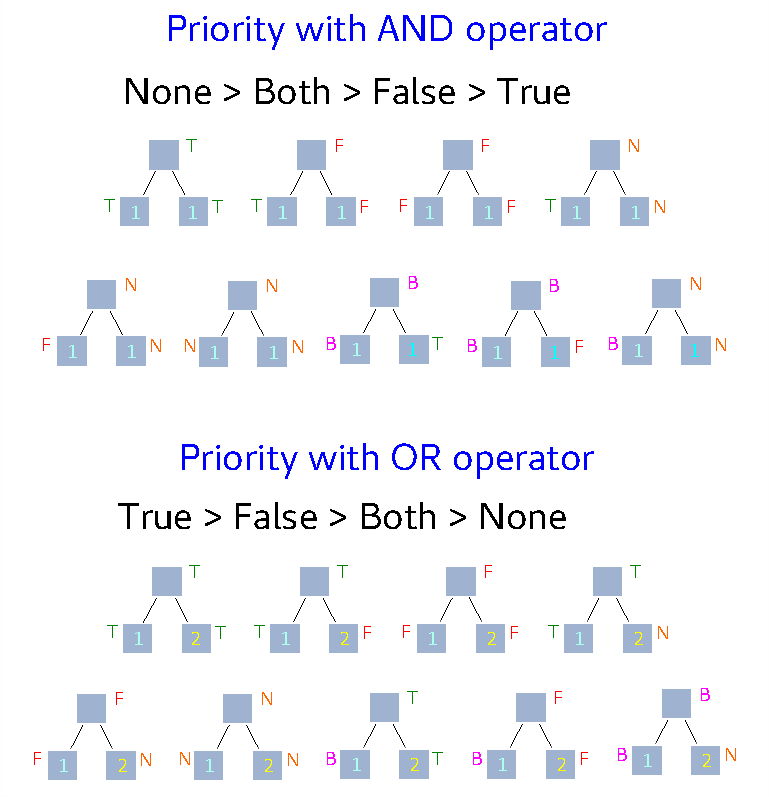
\includegraphics[width=\textwidth]{img/four_values_priorities_rules.pdf}
    \caption{ Règle de priorité pour l'inférence de multiple valeurs de vérité à travers un graphe "et/ou". }
    \label{fig:four_truth_values}
\end{shadedfigure}


\subsection{Application}
Ce travail a abouti sur une première implémentation de l'outil qui a été présenté lors de la conférence \texttt{RULEML2015}. En plus de pouvoir raisonner avec une logique multivaluée, le système est réactif à l'introduction de nouveaux faits de sorte que seules les nouvelles conséquences sont recalculées.

\cleardoublepage
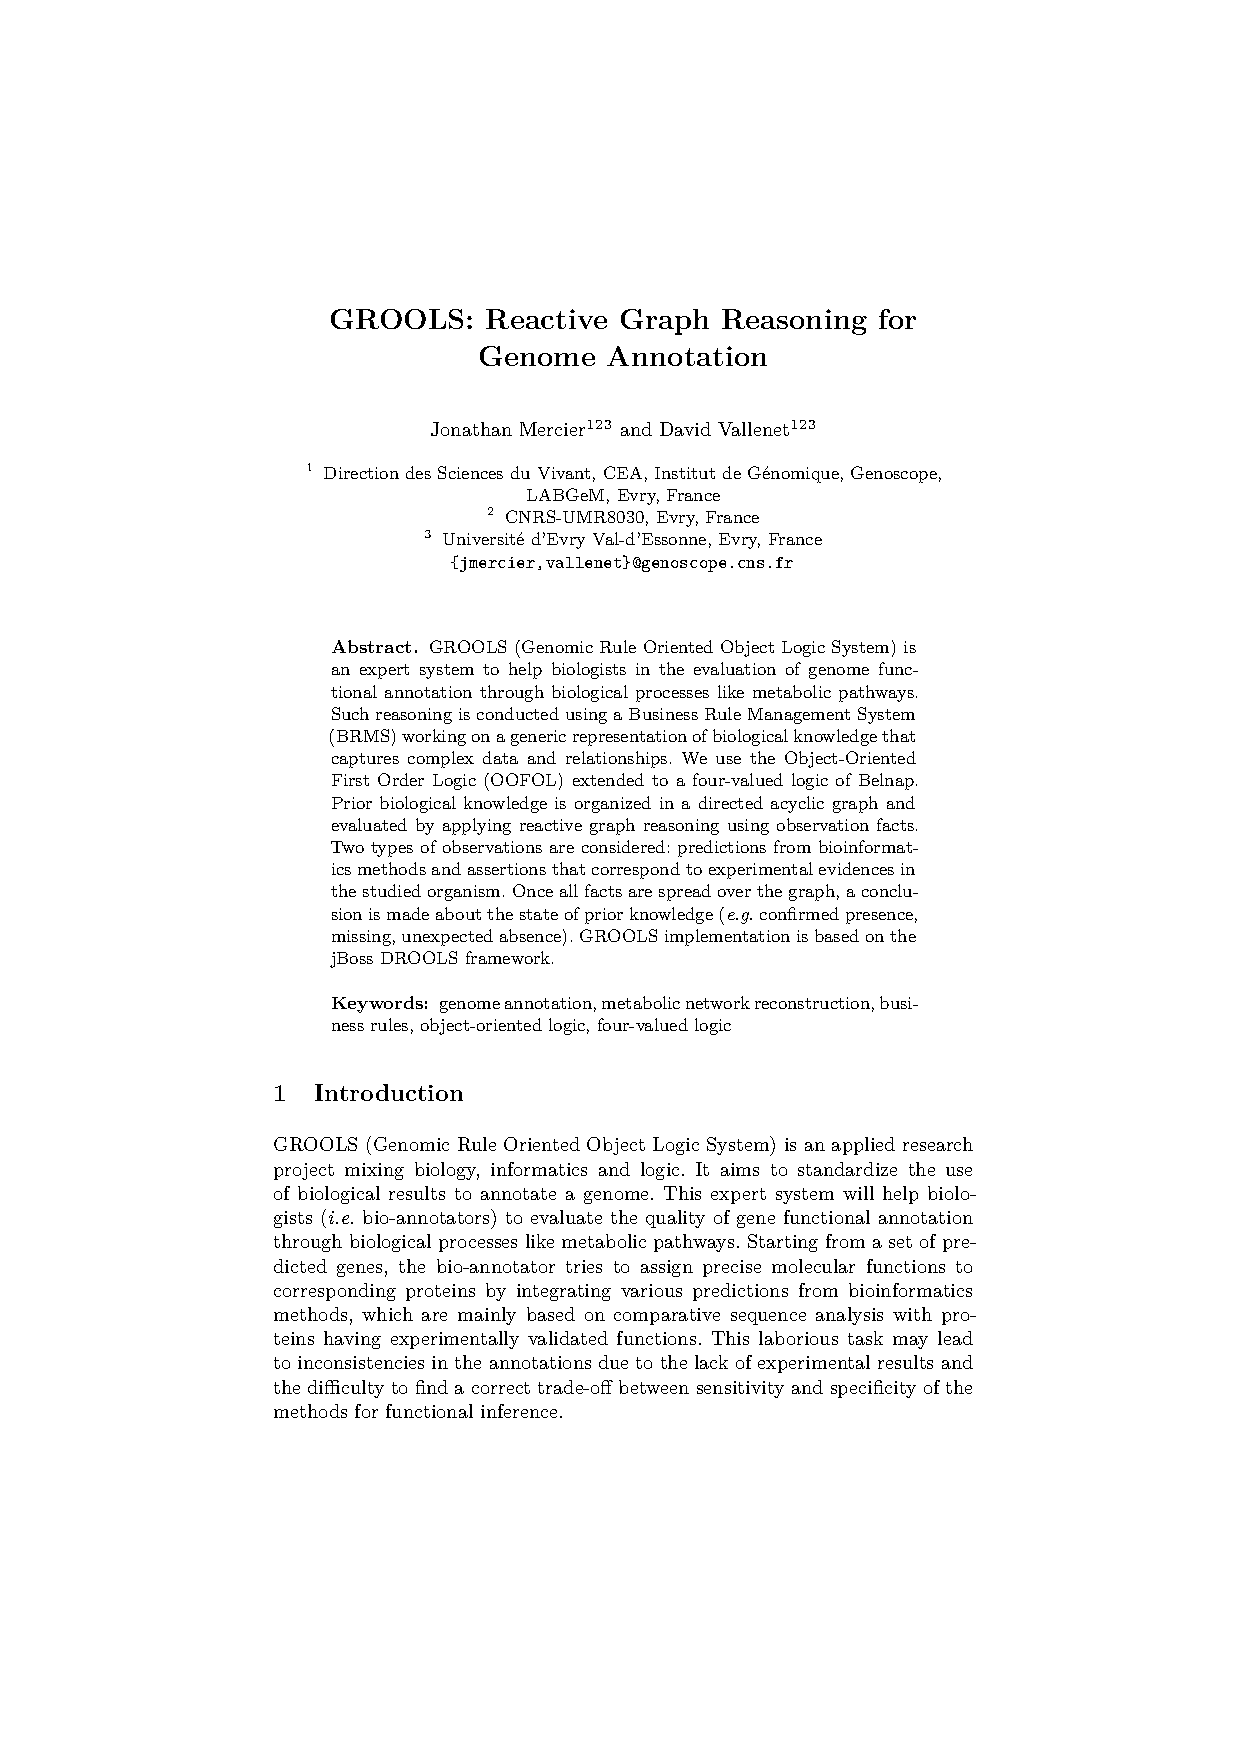
\includepdf[pages=-]{img/GROOLS__Reactive_Graph_Reasoning_for_Genome_Annotation.pdf}

\chapter{GROOLS: un système expert pour l'annotation fonctionnelle}

\section{Raisonnement sur des ensembles de valeurs de vérité}

La logique à quatre valeurs a ses limites lorsque l'on raisonne sur un graphe hiérarchique de connaissances. En effet, dans certains cas qui impliquent au moins deux concepts équivalents, il n'est pas possible de suggérer le chemin le plus plausible comme montré dans la \cref{fig:grools_belnap}. Bien que, si l'on prête attention aux concepts feuilles du graphe (les unités fonctionnelles), intuitivement on choisirait le variant avec la plus grande proportion de fonctions prédites.

\begin{shadedfigure}[H]
	\begin{subfigure}[t]{.48\textwidth}
		\centering
		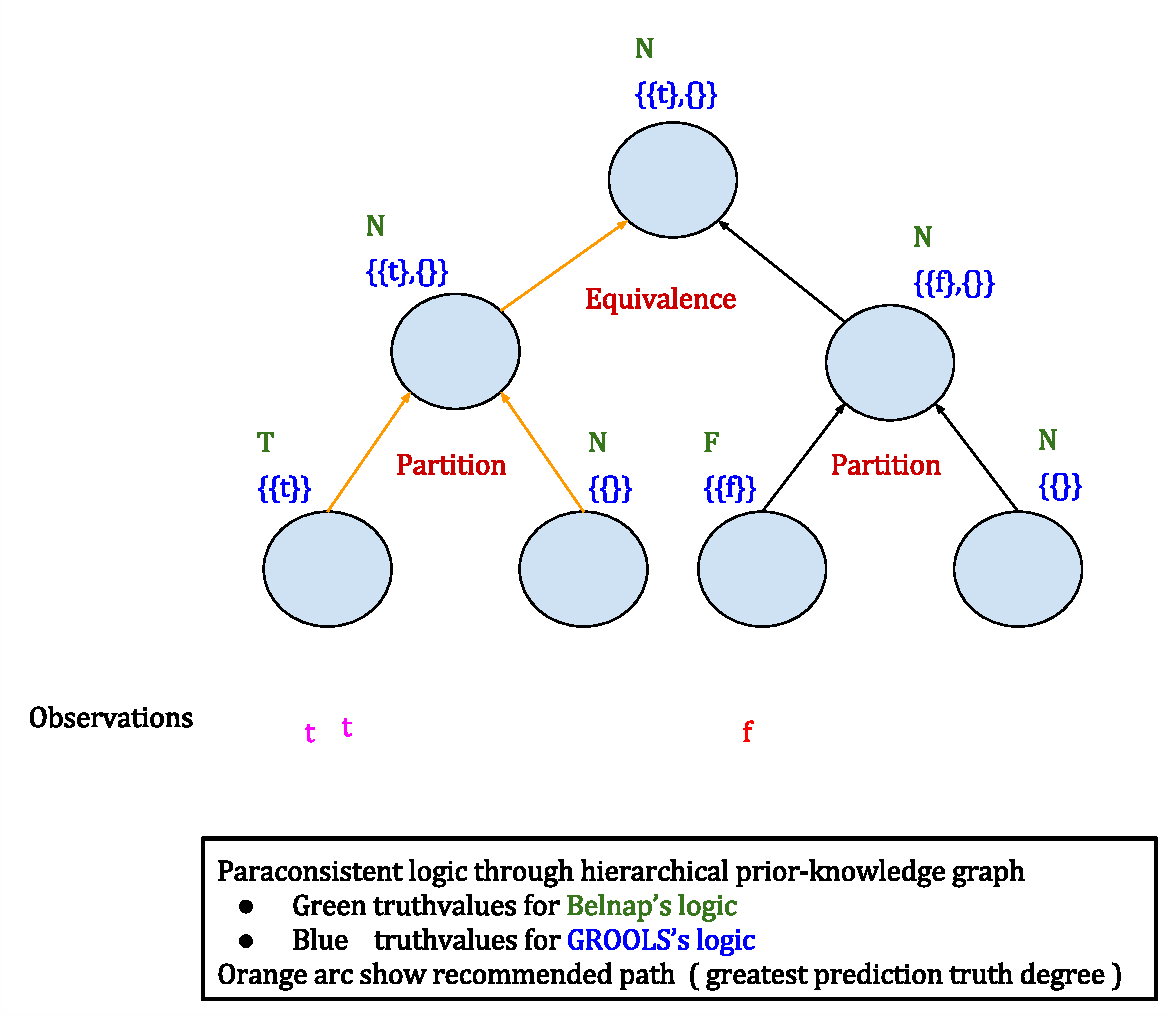
\includegraphics[width=\textwidth]{img/GROOLS_vs_belnap_1.pdf}
		\caption{Avec la logique de Belnap, il n'est pas possible de suggérer le chemin le plus vraisemblable lorsqu'il y a des valeurs incertaines.}
		\label{fig:grools_belnap_1}
	\end{subfigure}
	\hfill
	\begin{subfigure}[t]{.48\textwidth}
		\centering
		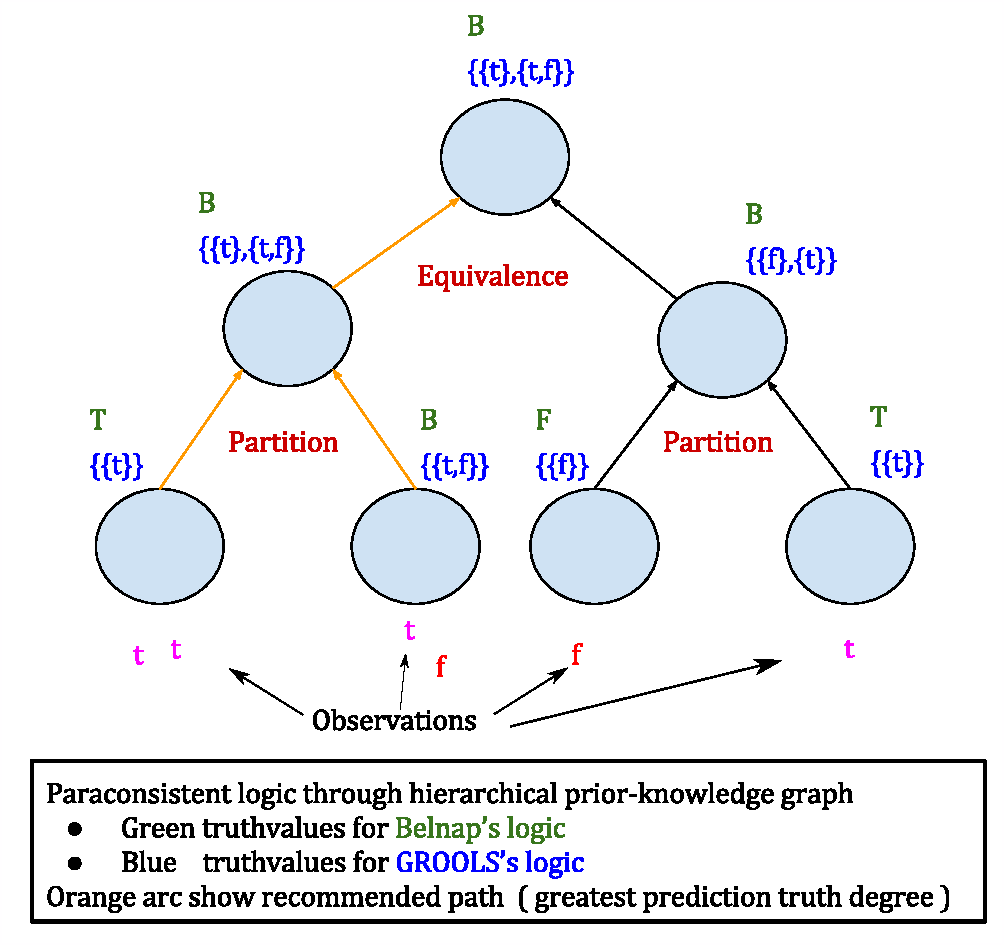
\includegraphics[width=\textwidth]{img/GROOLS_vs_belnap_2.pdf}
		\caption{Avec la logique de Belnap, il n'est pas possible de distinguer le chemin avec le plus grand degré de véracité. }
		\label{fig:grools_belnap_2}
	\end{subfigure}
	\label{fig:grools_belnap}
\end{shadedfigure}

J'ai réalisé que la notion de valeur contradictoire décrite par Belnap ("Both") était en fait un ensemble de valeurs de vérité vrai-et-faux. Par conséquent, essayer de représenter un ensemble de plusieurs valeurs dans une seule valeur de vérité "Both" est approximatif.

Sur la même idée, j'ai constaté que, dans mon cas d'application, j'avais des ensembles d'observations. En effet, des observations provenant de multiples sources peuvent désigner un même concept. D'autre part en laboratoire, une même expérience peut être répétée une ou plusieurs fois. Il y a également le cas de figure d'équipes différentes qui ont réalisées la même expérience. Dans ces deux cas, de multiples observations sont reliées à une même théorie. Elles peuvent avoir des résultats expérimentaux différents. Par conséquent, les ensembles de valeurs de vérité possibles, en lien avec les ensembles d'observations sont : $\{t\} \{f\} \{t,f\} \{\emptyset\}$, respectivement ensemble : vrai, faux, vrai-et-faux, ni-vrai-ni-faux. 

Quant aux connaissances \textit{a priori}, elles sont observables par de multiples ensembles d'observations dus à la notion de composition de concepts. Par exemple, une connaissance \texttt{A} est composée d'une connaissance \texttt{B} et d'une autre \texttt{C}. Les observations relatives à la connaissance \texttt{A} sont l'union des ensembles d'observations de \texttt{B} et de \texttt{C}. C'est donc un ensemble d'ensembles\footnote{En anglais on utilise le terme de "powerset"} d'observations. La combinaison des quatre ensembles d'observations ($\mathbb{P}(2)$) donne seize ensembles ($\mathbb{P}(4)$). Ces seize combinaisons permettent de mieux représenter la population des observations liées à un concept. Ces ensembles permettent de faire des choix sans approximation lors du raisonnement. Peu de temps après avoir décrit cette combinatoire d'ensembles, j'ai noté l'existence d'un travail de recherche similaire réalisé par \citeauthor{shramko2005some}. Ils décrivent ces mêmes ensembles, nommés les valeurs de vérité généralisées. Ces valeurs ont été présentées dans la partie \nameref{par:logic_multivalued}  de ce mémoire (cf. la \cref{fig:sixteen_truth_values}).

\needspace{5\baselineskip}
\begin{tasks}[counter-format = {tsk[1].},label-offset = {0.8em},label-format = {\bfseries}](4)
	\task $\{\emptyset\}$
	\task $\{\{\emptyset\}\}$
	\task $\{\{t\}\}$
	\task $\{\{f\}\}$
	\task $\{\{t,f\}\}$
	\task $\{\{t\},\{t,f\}\}$
	\task $\{\{\emptyset\},\{t\}\}$
	\task $\{\{\emptyset\},\{f\}\}$
	\task $\{\{t\},\{f\}\}$
	\task $\{\{f\},\{t,f\}\}$
	\task $\{\{\emptyset\},\{t\},\{t,f\}\}$
	\task $\{\{t\},\{f\},\{t,f\}\}$
	\task $\{\{\emptyset\},\{t\},\{f\}\}$
	\task $\{\{\emptyset\},\{t,f\}\}$
	\task $\{\{\emptyset\},\{f\},\{t,f\}\}$
	\task $\{\{\emptyset\},\{t\},\{f\},\{t,f\}\}$
\end{tasks}

Les observations dans GROOLS sont dissociées en deux types : prédiction et expectation. Ainsi, chaque théorie possède deux espaces distincts (l'espace des prédictions et l'espace des expectations). Ces espaces sont représentés par des ensembles de valeurs de vérité $\mathbb{P}(4)$ . Les prédictions sont inférées vers les connaissances généralistes, c'est-a-dire des unités fonctionnelles vers les voies métaboliques et inversement pour les expectations. Lorsqu'au moins deux chemins équivalents se présentent, l'inférence des prédictions et des expectations peut être conditionnée selon le degré de véracité ou de fausseté. Par exemple, l'expectation d'une voie métabolique attendue sera propagée sur le ou les variant(s) ayant des prédictions avec le plus grand degré de croyance : si un variant \texttt{A} est représenté par l'ensemble $\{\{t,f\}\}$ et un variant  \texttt{B} est représenté par l'ensemble $\{\{f\}\}$ alors le variant \texttt{A} est suggéré.

Un avantage de cette représentation en ensembles est la possibilité de calculer un degré de croyance, que l'on appelle également degré de véracité. Pour ce faire, le calcul est composé de quatre étapes et débute par les valeurs booléennes, c'est-à-dire les valeurs de vérités : vrai et faux. Le postulat de départ est le suivant : la valeur vrai "\texttt{t}"  vaut 1 sur l'échelle de la véracité et 0 pour la valeur faux "\texttt{f}".

\needspace{25\baselineskip}
\begin{enumerate}
    \item Constitution des ensembles $\mathbb{P}(2)$ (i.e $\{\emptyset\},\{t\},\{f\},\{t,f\}$)
    \item Calcul du degré de vérité pour les ensembles  $\mathbb{P}(2)$.
    \begin{equation*}
    \frac{1}{n} \sum_{i=1}x_{i}
    \begin{cases}
    \{\emptyset\} \to \frac{0}{1} = 0 \\
    \{t\} \to \frac{1}{1} = 1 \\
    \{f\} \to \frac{0}{1} = 0 \\
    \{t,f\} \to \frac{1+0}{2} = 0.5
    \end{cases}
    \end{equation*}
    \item Constitution des ensembles $\mathbb{P}(4)$ (i.e les 16 ensembles).
    \item Calcul du degré de vérité pour les ensembles  $\mathbb{P}(4)$ . Chaque sous-ensemble est représenté par son degré de vérité (ex: $\{\{t\}.verit\acute{e},\{f\}.verit\acute{e}\}$). Quelques exemples:
    \begin{equation*}
    \frac{1}{n} \sum_{i=1}x_{i}.verit\acute{e}
    \begin{cases}
    \{\{t\}\}                               &\to \frac{1}{1} = 1 \\
    \{\{t,f\}\}                             &\to \frac{1}{2} = 0.5 \\
    \{\{t\},\{t,f\}\}                       &\to \frac{1+0.5}{2} = 0.75 \\
    \{\{\emptyset\},\{t\}\}                 &\to \frac{0+1}{2} = 0.5 \\
    \{\{t\},\{f\}\}                         &\to \frac{1+0}{2} = 0.5 \\
    \{\{\emptyset\},\{t\},\{f\},\{t,f\}\}   &\to \frac{0+1+0+0.5}{4} = 0.125
    \end{cases}
    \end{equation*}
\end{enumerate}

Cette méthode permet de calculer également le degré de fausseté (i.e non-croyance). Pour des ensembles  $\mathbb{P}(2)$ et au delà, on peut calculer (i) le degré de contradiction (1 pour le sous-ensemble $\{t,f\}$ et 0 pour les autres), (ii) le degré d'incertitude (1 pour le sous-ensemble $\{\emptyset\}$ et 0 pour les autres).

\begin{shadedfigure}[H]
    \centering
    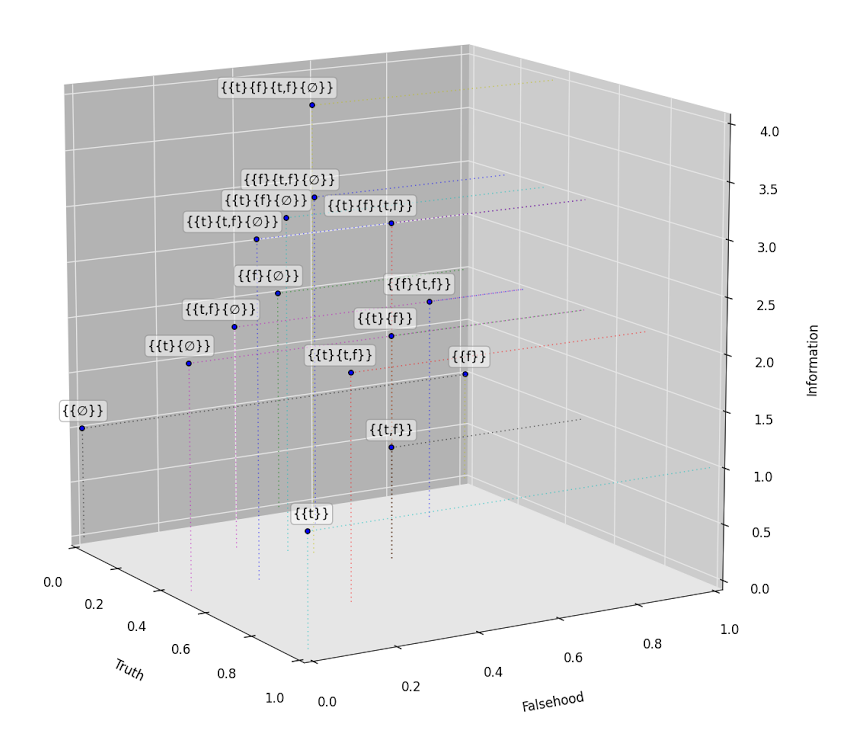
\includegraphics[width=\textwidth]{img/set_3d.png}
    \caption{Représentation des ensembles  $\mathbb{P}(4)$ selon 3 axes, (i) vérité, (ii) fausseté, (iii) information (i.e le nombre de sous-ensembles).}
    \label{fig:set3d}
\end{shadedfigure}

\section{La méthode GROOLS}\label{sec:methode}

Mes recherches m'ont conduit à développer une méthode pour représenter et raisonner sur des ensembles de valeurs de vérité. Ces ensembles sont utilisés pour décrire les prédictions et les expectations des différentes théories.

J'ai développé un système expert, nommé \texttt{\gls{GROOLS}}, utilisant une logique paracohérente pour assister le biocurateur dans le processus de l'annotation fonctionnelle des protéines. \texttt{\gls{GROOLS}} permet d'évaluer la complétion et la cohérence des fonctions prédites au travers de processus biologiques, par exemple les voies métaboliques. A la fin du raisonnement, la méthode émet des conclusions sur les différents composants des processus. Par l'utilisation d'expectations envers l'organisme étudié, ces conclusions permettent d'informer le biologiste sur les composants confirmés, manquants, ambigus, etc. La méthode et les résultats sont décrits dans l'article suivant qui a été soumis au journal Bioinformatics en Mars 2017.

\cleardoublepage
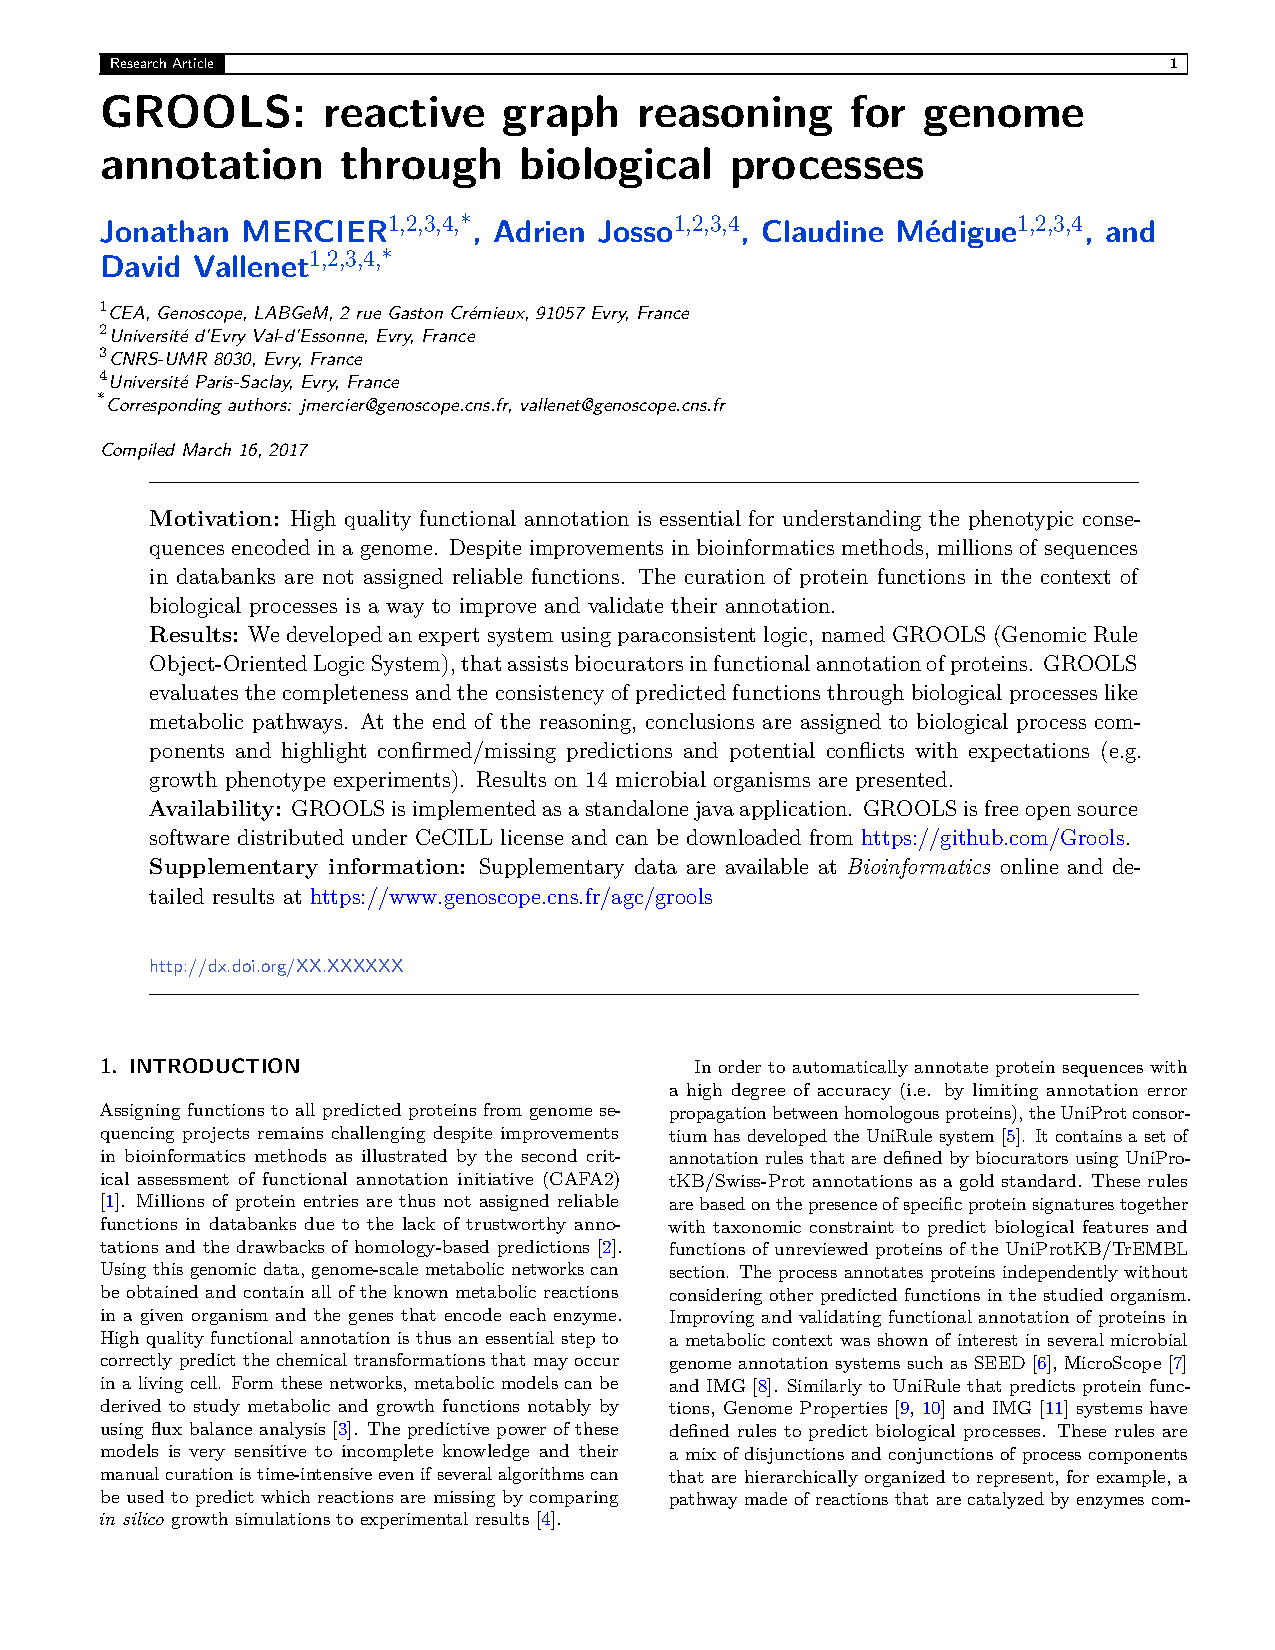
\includepdf[pages=-]{img/GROOLS_bioarchiv.pdf}

\section{Discussion}
\subsection{Difficultés rencontrées}
L'implémentation du raisonnement dans le moteur de règles \texttt{DROOLS} a engendré quelques difficultés. La première est la non maîtrise du moment de l'évaluation d'un groupe de faits par une règle. Il faut savoir que seul le moteur de règle décide quelle règle doit être activée à tel moment. Les conflits de priorité entre les règles sont gérés par \texttt{DROOLS} en interne par un système de résolution de conflits. Il arrive, par exemple, que deux règles peuvent s'activer à un même moment car elles évaluent les mêmes faits. Pour illustrer un tel cas, considérez les deux règles suivantes:

\needspace{25\baselineskip}
\begin{lstlisting}[style=drl-style,caption=conflit]
rule "Direct prediction"
when
	$k : PriorKnowledge(  )
	$p : Observation( type = Type.PREDICTION,  value != $k.prediction )
then
	modify($k){
		prediction = $p.value
	}
end

rule "Infer prediction from children PriorKnowledge"
when
	$k    : PriorKnowledge(  )
	$child: PriorKnowledge( $k memberOf parents, prediction not in $k.prediction )
then
	modify($k){
		prediction += $child.prediction
	}

end
\end{lstlisting}

Ces deux règles vont se déclencher dès qu'une connaissance \textit{a priori} est ajoutée ou mise à jour. Par contre, l'ordre de déclenchement n'est pas maitrisable ce qui peut changer complétement le résultat. Par exemple, en supposant que la connaissance \textit{a priori}  possède une prédiction $\{\{t,f\}\}$, le concept enfant  $\{\{f\}\}$ et l'observation $\{\{t\}\}$, si la règle 1 se déclenche avant la 2, alors la prédiction sera $\{\{t\},\{t,f\}\}$. En revanche, si la règle 2 est activée avant, on obtient la prédiction  $\{\{t\}\}$.

Il existe le système de "\texttt{salience}" qui attribue un poids à une règle et ainsi priorise les règles les unes par rapport aux autres.  Cependant, avoir recours à la "\texttt{salience}" est souvent le signe d'un raisonnement mal formulé.

De plus dans un système réactif, la modification de la connaissance \textit{a priori} induite par les deux règles précédentes provoque une boucle dans le raisonnement car elles vont perpétuellement s'activer réciproquement. Pour éviter de tels cas de figure, il est nécessaire de rendre les règles plus précises. Pour cela, de nouvelles règles doivent être ajoutées afin de couvrir la diversité des problèmes. En conséquence, il y a un risque plus important de collision de règles. À chaque nouvel ajout de règles, il faut s'assurer de l'absence de conflit vis-à-vis de toutes les autres règles et de la diversité des faits possibles. Tout ceci rend la construction d'un raisonnement réactif très compliqué. Dans le cas précédemment décrit, la règle  pour l'inférence de la  prédiction "directe"  peut être divisée en deux règles : la première pour inférer l'ensemble des observations lorsque la connaissance \textit{a priori} ne possède aucune prédiction ($\{\{\emptyset\}\}$) et une seconde lorsque la connaissance \textit{a priori} possède au moins une prédiction, les observations directes viennent s'ajouter à l'ensemble des prédictions.

Une des grandes difficultés lorsque l'on travaille avec ce type d'outil, c'est que nous obtenons un résultat final sans être en mesure d'identifier quelles règles ont été activées et pourquoi elles l'ont été. Le système \texttt{DROOLS} fournit un système de trace des évènements mais il est compliqué à analyser. Il n'indique pas pourquoi la règle est activée et encore moins pourquoi elle n'a pas été activée. En effet, même pour un petit jeu de données, les traces produisent un volume important d'évènements, ce qui demande du temps pour les analyser et comprendre les choix du raisonneur. Il est donc extrêmement laborieux d'analyser les traces: par exemple, certains cas non souhaités sont dus à l'activation d'une succession de règles.

A ces difficultés de coordination des différentes règles, s'ajouté également des erreurs critiques que j'ai rencontré dans le système \texttt{DROOLS}. Ces problèmes ont été rapportés aux développeurs quand j'étais en mesure de fournir un exemple minimal reproduisant le "bug". Les deux liens ci-dessous correspondent à des bugs que j'ai découvert et qui ont été rapportés à l’équipe de développement de \texttt{DROOLS} :
\begin{itemize}
	\item \url{https://issues.jboss.org/browse/DROOLS-809}
	\item \url{https://issues.jboss.org/browse/DROOLS-809}
\end{itemize}
 
Ainsi, à la difficulté d'exprimer des règles sans conflit les unes par rapport aux autres, se sont ajoutées des contraintes supplémentaires dans l’expression de ces règles, imposées par le système suite aux "bugs" rencontrés.

Malgré toutes ces difficultés, ce travail a abouti à une version fonctionnelle, accessible à l'adresse : \url{https://github.com/Grools/grools-drools-checker} . Cependant, le raisonneur \texttt{DROOLS} a montré ses limites pour raisonner sur des données hiérarchiques. Les règles et les faits ne sont pas utilisés dans un ordre optimum vis-à-vis du graphe de connaissances. De nombreuses ré-activations de règles sont observées, induisant un temps de calcul accru. De plus, l'évaluation de collections de faits (essentielle pour le raisonnement) est très couteuse pour le raisonneur \texttt{DROOLS}. Ces opérations empêchent le raisonneur d'activer les règles de façon efficace. Elles peuvent s'écrire avec les expressions suivantes : \lstinline[style=drl-style]$Set() from collect(...)$, \lstinline[style=drl-style]$forall(...)$, \lstinline[style=drl-style]$Number() from accumulate(...)$\footnote{Des exemples sur ces expressions sont accessibles à l'adresse suivante: \url{http://blog.athico.com/2007/06/chained-from-accumulate-collect.html}.}. Ces instructions recréent des collections d'objets à chaque réactivation d'une règle, ce qui est inefficace. Ainsi, le raisonnement prend entre deux et neuf heures de calcul selon la quantité de faits et la représentation des connaissances qui est utilisée (\texttt{Genome Properties} ou UniPathway). Il était donc nécessaire d'ajouter des règles permettant d'ordonner l'activation des règles dédiées au raisonnement et, ainsi, minimiser le nombre de réactivations vis-à-vis du graphe de connaissances. J'avais commencé ce travail, mais là encore, j'ai été confronté à des comportements indésirables de la part du raisonneur. J'ai établi au cours de ces trois années de bonnes relations avec l'équipe de développement de \texttt{DROOLS} . À la suite de la présentation  des nouveaux problèmes rencontrés, ils m'ont proposé de travailler conjointement pour apporter des corrections dans la version suivante. Malheureusement, le temps qui m'était imparti ne me permettait pas d'investiguer de façon plus approfondie dans le moteur d'inférence de DROOLS, de trouver une solution, de la faire valider et d'attendre la nouvelle version.

C'est la raison pour laquelle, j'ai ré-écrit un moteur de raisonnement réactif dans le langage Java. Afin de rester dans le contexte d'une programmation déclarative, les règles ont été écrites en utilisant le paradigme de la programmation fonctionnelle\footnote{\url{https://fr.wikipedia.org/wiki/Programmation_déclarative}}. Ce projet open source est appelé \texttt{grools-reasoner} (\url{https://github.com/Grools/grools-reasoner}). Cette bibliothèque a été utilisée pour l'exploration des voies métaboliques de 14 génomes bactériens dans l'article présenté dans la \namecref{sec:methode} \cref{sec:methode}. L'outil s'est montré capable de raisonner sur tout un génome en moins d'une minute.

La bibliothèque est modulaire, elle peut être utilisée pour différents besoins :\nolisttopbreak
\begin{itemize}
	\item \texttt{grools-application}: exploration du métabolisme à travers les modèles \texttt{Genome Properties} et \texttt{UniPathway}  (\url{https://github.com/Grools/grools-application}).
	\item \texttt{grools-interpreter}: chargement d'un ancien raisonnement et exécution des requêtes pour l'analyse des faits (\url{https://github.com/Grools/grools-interpreter}).
	\item et d'autres à venir\ldots
\end{itemize}

\subsection{Logique paracohérente}
Lorsqu'il est nécessaire de raisonner dans un monde avec des incertitudes et des incohérences, la logique à quatre valeurs de \textit{Belnap} semble suffisante. En effet, les valeurs de vérités TRUE, FALSE, BOTH et NONE couvrent la notion de vrai, faux, contradictoire et incertain. Cependant, lorsque l'on regarde de plus près la table de vérité  (voir la section \nameref{par:logic_multivalued}  \cref{tab:belnap_truth_table}), certaines combinaisons peuvent se montrer contre-intuitives, par exemple: $ BOTH \lor  NONE = TRUE$ et $ BOTH \land NONE = FALSE$. Le premier cas  peut se représenter de la sorte: 
\begin{enumerate}
    \item Un variant \texttt{A} d'une voie métabolique possède des prédictions contradictoires (BOTH)
    \item Un autre variant \texttt{B} a une absence de prédiction (NONE)
    \item La voie métabolique va être prédite (TRUE), d'après la table de vérité de \textit{Belnap}, par le calcul de la proposition \texttt{A} OU \texttt{B}.
\end{enumerate}
Ce résultat non-intuitif est dû à une impossibilité d'exprimer plus de quatre états et ne peut pas, ainsi, faire la distinction entre des valeurs de vérité à part entière et des ensembles de valeurs de vérité. Cette logique essaye de représenter l'ensemble $\{t,f\}$ qui comporte deux valeurs en une seule, ce qui inexorablement amène à des approximations. Cette logique ne peut donc pas être utilisée avec un graphe de connaissances sans conduire à des  imprécisions comme l'illustre la \cref{fig:grools_belnap_1} et la  \cref{fig:grools_belnap_2}. 

Mon interprétation est que ces ensembles de valeurs de vérité ne sont pas des valeurs de vérité. Par conséquent, il ne faut pas essayer d'étendre la logique classique à d'autres valeurs de vérités. Ce point de vue rejoint celui émis par \citeauthor{dubois2008ignorance} dans \citetitle{dubois2008ignorance}\cite{dubois2008ignorance}. La logique multivaluée de Belnap a introduit une confusion entre valeur de vérité et l'état d'information.


\end{refsegment}


    
\begin{refsegment}
\chapter{Vers une compréhension des voies métaboliques}
\subbibliography
\end{refsegment}
    
    \cleardoublepage
    \thispagestyle{empty}
    \printbibliography
    \cleardoublepage
\end{document}